\documentclass[11pt]{ucdavisthesis}
%\documentclass[11pt,draft]{ucdavisthesis}

\usepackage{amsmath}
\usepackage{amssymb}
\usepackage{siunitx}
\sisetup{
  retain-unity-mantissa=false
}
\usepackage{booktabs}
\usepackage[Q=yes]{examplep}
\usepackage{graphicx}
\usepackage[
    abbreviate=false,
    backend=biber,
    backref=true,
    refsection=chapter,
    sortcites=true,
    sorting=nyt,
    sortlocale=en_US,
    style=numeric-comp
]{biblatex}
\addbibresource{library.bib}
\defbibheading{subbibliography}{\section*{References for Chapter \ref{refsection:\therefsection}}}

\usepackage{caption}
\usepackage{longtable}
\captionsetup{margin=10pt,font=small,labelfont=bf}

\usepackage{tikz}
\usetikzlibrary{arrows,calc,shapes,positioning}
\usepackage{pgfplots}
\pgfplotsset{compat=newest,compat/show suggested version=false}

% hyperref should come after biblatex (according to biblatex documentation),
% and it should be loaded last (according to hypperef documentation.
\usepackage[
    colorlinks=true,
    pdfencoding=auto,
    pdfauthor={Dale Lukas Peterson},
    pdfkeywords={bicycle; dynamics; control; linearization; constraints; system identification},
    pdftitle={Bicycle dynamics: modelling and experimental validation},
    xetex
]{hyperref}

\newcommand{\bm}[1]{\mathbf{#1}}
\newcommand{\uv}[2]{\hat{\mathbf{#1}}_{#2}}
\allowdisplaybreaks[1]
\begin{document}

\title{Bicycle dynamics: modelling and experimental validation}

\author{Dale Lukas Peterson}

\authordegrees{B.S. (University of California Santa Barbara) 2004 \\
               M.S. (University of California Davis) 2007}

\officialmajor{Mechanical Engineering}

\graduateprogram{Mechanical and Aerospace Engineering}

\degreemonth{September}

\degreeyear{2013}

\committee{Mont Hubbard, Chair}{Ronald A. Hess}{Fidelis O. Eke}{}{}

\dedication{\textsl{To my family.}}

\acknowledgments{\label{acknowledgements}
This work would not have been possible without the support of many people.
First and foremost, I would like thank my parents, John and Lyn. They have been
there for me at every stage of my life and I am thankful for their support,
love, care, and for inspiring me to be inquisitive about the world around me.
Next, I would like to thank my fianc\'ee Cassandra Ann Paul, who has been
essential to this dissertation. Cassandra has encouraged me when I needed it
most, chastized me when I deserved it, and kept me positive throughout a very
stressful final year of graduate school. Cassandra is a reminder of what is
important in life, and I look forward to building our lives together.

I have had many excellent teachers in my life and this dissertation is a
reflection of them me. I would to thank Joan Owen, Joyce Hodgkinson, and
Elizabeth Terwilliger for their thoughtful and forward thinking work during my
early years at Tam Creek School. They planted the seeds of civic duty and
environmental stewardship in many young children and I am thankful to have been
one of their students. I would like to thank my high school chemistry teacher,
Nina Tychinin, for encouraging me to explore my interests in science. Near the
end of my undergraduate education, after returning from a two year activation
with the United States Marine Corps, I enrolled in an applied dynamics course
with Dr. Steven Shaw and a control systems course with Dr. Jo\~{a}o P.
Hespanha. These two teachers are directly responsible for igniting my
fascination with dynamics and control, and I would like to thank them for
careful and inspired presentation of these two beautiful subjects.

I would like to thank my Ph.D. advisor Dr. Mont Hubbard for his patience and
clarity of thought, and for the many discussions about dynamics, control, and
bicycles. It has been a true pleasure to work with Mont and I am grateful to
have learned so much from him; I hope I was as good a student to him as he was
an advisor to me. I would like to thank Dr. Ron Hess for his support and
feedback throughout the period of the NSF grant and specifically for his help
with design of the control system of the robotic bicycle. I would like to thank
Dr. Fidelis Eke for his extremely clear presentation of multibody dynamics and
Kane's method in particular. I would like to thank Dr. James
Crutchfield for his inspirational course on nonlinear dynamics in which I was
first exposed to the Python programming language.

The work of Dr. Arend L. Schwab, Dr. Jeremy Papadopoulos, Dr. Andy Ruina, and
Dr. Jaap Meijaard has had a large impact on this work. Their clarity of
presentation and the many thoughtful discussions we have had about bicycle
dynamics and control have significantly improved my understanding of bicycles
and dynamics. I would like to extend special thanks to Dr. Arend Scwab and Dr.
Jeremy Papadopoulos for the many in-depth discussions and emails we have had.
It is my hope that the work in this dissertation is an important addition to
the groundwork that you and many others have laid.

There are several students I would like to thank. First and foremost, I would
like to thank my friend Jason Moore. Jason has enriched my life both inside and
outside the walls of the academy (which we are both trying to tear down). I
have enjoyed discussing bicycles, religion, computers, math, and philosophy
with Jason and I credit him with keeping me on my toes and testing my views on
the world. Thomas Johnston was a great companion in graduate school, and I am
thankful for the many hours of discussion of dynamics we have had. I would like
to thank all of the members, past and present, of the Sports Biomechanics
Laboratory.

I would like to thank Ond\v{r}ej \v{C}ert\'{i}k for his substantial commitment
to symbolic mathematics with the SymPy project and for helping me build a tool
with which to study dynamics. Ond\v{r}ej has demonstrated excellent leadership
and has created a wonderful community for symbolic mathematics.  His
selflessness and commitment have helped to make my dissertation possible.

In the summer of 2011 Gilbert Gede and I worked closely to add classical
mechanics functionality to the SymPy project. It was also during this time that
the ideas for Chapter 3 of this dissertation were planted and initially
developed. Gilbert's hard work and collaboration on the development of these
ideas is greatly appreciated.

A large number of people contributed to the success of the robot bicycle. Benny
Brown provided hours of much need electrical engineering experience and know
how. Kenny Koller helped me understand embedded systems and provoked a lot of
thought about careful design of software which interacts directly with hardware
resources. Kenneth Lyons helped with steer angle calibration, and Derek Pell
helped fabricate a number of components used for measuring the physical
parameters of the bicycle. I appreciate all of your help.

Oliver Z. Lee deserves special recognition for his help with the robot bicycle.
Oliver and I worked shoulder to shoulder for the first 7 months of 2013 and we
came to know each other quite well. Oliver's contribution to this dissertation
was significant and essential; in particular, the robot bicycle would not have
balanced had it not been for his hard work, focus, and impressive skills in
software and control systems.

Finally, I would like to thank Martin Hansen, Ron Blinn, Tony Merz, Erik
Gambera, Allen Donhauser, and Steve Wyrostok from Sunshine Bicycle Center for
all the support and interesting discussion we have had over the last eighteen
years. My fascination with bicycles was kindled by discussions we had at the
shop.

This material is partially based upon work supported by the National Science
Foundation under Grant No. 0928339. Any opinions, findings, and conclusions or
recommendations expressed in this material are those of the author(s) and do
not necessarily reflect the views of the National Science Foundation.

}

\abstract{This dissertation explores bicycle dynamics through an extension of the Whipple
bicycle model and validation of the model equations equations of motion through
the implementation of a robotic bicycle. An extended Whipple bicycle model is
presented which makes uses of a unique set of physical parameters based on
cylindrical gyrostats. The nonlinear equations of motion for this model are
derived, linearized, and validated against a set of benchmark model parameters.
A general formulation for the linearization of a system with configuration and
velocity constraints is presented, and is demonstrated on an idealized rolling
disk. The method of linearization is directly applicable to the equations of
motion which result from the application of Kane's method. The linearization
procedure is used to formulate the linear state space equations of motion for
the bicycle model, which are then used as the plant model to design the robotic
bicycle control system. The mechanical, electrical, and software aspects of the
robotic bicycle are presented, along with representative results from a set of
experiments.

}

\makeintropages

\chapter{Mathematical model of bicycle motion}

\section{Introduction}

\section{Physical parameters}

\section{Kinematics}

\section{Dynamics}


\printbibliography[section=1,heading=subbibliography]
\chapter{Mathematical model of bicycle motion} \label{chapter2}

\section{Introduction}
The bicycle model we use assumes the bicycle is composed of four rigid bodies:
two wheels, a frame, and a fork. These rigid bodies are assumed to be connected
by three frictionless revolute joints: one between the rear wheel and frame,
one between the front wheel and fork, and one between the bicycle frame and the
fork. The rigid wheels are modelled as torii which make point contact with the
ground plane. The frame and fork are each assumed to to be inertially
symmetric about in their respective $XZ$ planes. The revolute joint connecting
the frame and fork is assumed to be parallel to the $Z$ axis of the
each respective body. It is assumed that each wheel mass center lies in the
$XZ$ symmetry plane of the body to which it is connected, and that each wheel
revolute joint axis is parallel to the $Y$ axis of each respective body.

\section{Bicycle parameters}
The physical parameters used to describe the four rigid bodies, their interface
with each other and the ground plane is of practical concern for several
reasons. The choice of parameters determines how many quantities must be
measured or calculated when characterizing a real bicycle; some parameters are
more difficult to measure than others. The choice of parameters has a direct
effect on the complexity of the equations of
motion~\cite{Wittenburg2008,Mitiguy2001}, and by extension, the computational
cost associated with simulating or performing stability analysis of the
equations. Most importantly, the choice of parameters can greatly affect the
ease of understanding how changing a single parameter affects the dynamics.
Finally, having a common, agreed upon set of parameters which permit direct
comparisons is very valuable in communicating results to others -- if
everybody uses different parameters to describe the same model, comparisons
become difficult and error prone. We refer to the parameters used
in~\cite{Meijaard2007} as the ``Meijaard parameters'' (this is not the first
use of this parameter set, but it is the most clearly presented and widely
distributed work describing the choice). The Meijaard parameters have been
adopted as the \textit{de facto} by many authors~\cite{Sharp2008}. They can be
measured reasonably simply~\cite{Moore2010b}, and many of the parameters are
familiar to those outside academic circles (i.e., the bicycle industry, and
everyday cyclists). Examples of commonly recognizable parameters available at
your local bike shop include wheelbase $w$, trail $c$, and steer axis tilt
$\lambda$. For these reasons, this choice of parameters is indispensable.

There are strong reasons to prefer other choices of parameters. The Meijaard
parameters are ideally suited to direct derivation of linearized equations of
motion, about the reference configuration (lean and steer equal to zero). The
reason for this is that the Meijaard parameters are defined with respect to the
bicycle \textit{reference configuration} and with respect to a set of body
fixed coordinates that are aligned with the inertial frame \textit{only in this
configuration}. Deriving nonlinear equations of motion with this parameter set
is cumbersome and requires a number of intermediate geometric quantities to be
introduced. Perhaps the most serious disadvantage of the Meijaard parameter set
is the coupling between the parameters. Consider, for example, a parameter
study investigating the effect of front wheel radius on stability.  Using the
Meijaard parameters, a naive approach might be to choose a set of parameters
and compare the eigenvalues for that set with the eigenvalues when only the
wheel front wheel radius is changed. Unfortunately, this does not represent the
act of taking a real bicycle (with some set of parameters) and simply changing
the front wheel to one with identical mass and inertia but different radius.
Changing the front wheel radius of a real bicycle changes the steer axis tilt,
wheelbase, trail, center of mass locations relative to the rear wheel contact,
and, by virtue of the inertia scalars being defined relative to an inertial
frame, six of the inertia scalars. Thus, if the goal of an analyst or designer
is to understand the difference between how front wheel radius affects a
bicycle stability (a reasonable goal), and that person uses the Meijaard
parameter set to describe the bicycle, no fewer than \textit{thirteen}
additional parameters must be adjusted: the wheelbase $w$, trail $c$, steer
axis tilt $\lambda$, the central inertia scalars $I_{\text{B}xx}$,
$I_{\text{B}zz}$, $I_{\text{B}xz}$, $I_{\text{H}xx}$, $I_{\text{H}zz}$,
$I_{\text{H}xz}$, and the scalars describing the center of mass locations of
the bicycle frame and the fork $x_\text{B}$, $z_\text{B}$, $x_\text{H}$, and
$z_\text{H}$. This coupling of parameters is the result of defining the
parameters with respect to the reference configuration. If the naive approach
is used anyway, and all other parameters are left unchanged as
in~\cite{Moore2008,Tak2010}, it must be realized that when comparing results
which have only one of these coupled parameters changed (e.g., front wheel
radius), one is actually comparing bicycles with different frame and fork
geometry, center of mass location, and mass distribution since these must be
changed (on a real bicycle) in order to keep the Meijaard parameters constant.
Stated simply, one is not comparing effect of only front wheel radius, but the
effect of changing the front wheel radius and thirteen other parameters. The
practical utility of such a comparison is dubious at best. While this issue
\textit{can} be addressed by carefully changing the thirteen coupled
parameters, to our knowledge, no parameter study to date has done this. This is
a rarely stated, but critical, downside of the Meijaard parameters.

The easiest way to remedy the issue of parameter coupling is to choose physical
parameters which can be defined independent of configuration. This is standard
practice in robotics: robot link lengths are defined relative to the previous
link in the chain, and mass and inertia properties of each link are defined
with respect to a link-fixed coordinate system which is independent of overall
robot configuration. The thirteen Meijaard parameters which are defined
relative to the reference configuration can be arranged into three groups and
addressed separately. First, the wheelbase $w$, trail $c$, and steer axis tilt
$\lambda$ can be replaced with three distances which are independent of
configuration, as in~\cite{Franke1990}. Two of these measure the perpendicular
distance between the wheel centers and the steer axis while a third measures
the distance parallel to the steer axis between the first two lines. Second,
the bicycle frame and fork center of mass locations relative to the rear wheel
ground contact ($x_\text{B}, z_\text{B}, x_\text{H}, z_\text{H}$
in~\cite{Meijaard2007}) can be replaced with parameters which are defined
relative to the rear and front wheel centers, respectively. Finally, the
central inertia scalars of the bicycle frame and fork ($I_{\text{B}xx},
I_{\text{B}zz}, I_{\text{B}xz}, I_{\text{H}xx}, I_{\text{H}zz}, I_{\text{H}xz}$
in~\cite{Meijaard2007}) can be replaced with inertia scalars defined relative
to body-fixed coordinate systems which are aligned with a features fixed in the
body (such as the steer and wheel axes).

This section carefully describes the physical parameters used to model the
bicycle. These parameters address the issues raised in the previous two
paragraphs and also reduce the number of parameters needed to describe the same
four rigid bodies. This reduction is possible because the inertial properties
of rear frame and rear wheel are independent of the orientation of the rear
wheel relative to the rear frame (and similarly for the front fork and front
wheel). This parameterization of the physical properties of the bicycle is
collectively referred to as the gyrostat parameters. Finally, we present the
conversion from the Meijaard parameters to the gyrostat parameters.

\subsection{Gyrostat parameters} \label{model:gyrostat_parameters}
A gyrostat is a mechanical system of one or more bodies which has the rigid
body property that its inertia scalars are time independent
constants~\cite{Wittenburg2008}. The most common example of such a system is a
motor with a rotor which is inertially symmetric about the spin axis. As the
rotor rotates relative to the frame of the motor, neither the location of the
mass center nor the combined inertia of the system changes. This type of
gyrostat is referred to as a cylindrical gyrostat~\cite{Mitiguy2001}. The two
body cylindrical gyrostat is typically described as being composed of a carrier
and a rotor. A bicycle wheel and frame or fork is exactly such a gyrostat.

To aid the discussion which follows, we present the relationship between the
parameters which fully describe a cylindrical gyrostat and the parameters which
fully describe the two composing bodies. First consider a carrier $A$ with a
set of mutually perpendicular axes $X$, $Y$, $Z$ intersecting at the mass
center $A^*$ of $A$. $A$ has mass $m_A$, and let $\uv{a}{x}, \uv{a}{y},
\uv{a}{z}$ be unit vectors parallel to $X$, $Y$, $Z$, respectively, and express
the inertia dyadic of $A$ for $A^*$ as $\bs{I}^{A/A^*} =
I_{Axx}\uv{a}{x}\uv{a}{x} + I_{Ayy}\uv{a}{y}\uv{a}{y} +
I_{Azz}\uv{a}{z}\uv{a}{z} + I_{Axz}(\uv{a}{x}\uv{a}{z} + \uv{a}{z}\uv{a}{x})$.
$A$ is inertially symmetric about the $XZ$ plane. Attached to $A$ with a
revolute joint is rotor $B$ with mass $m_B$. Fixed to $B$ is a set of
mutually perpendicular axes $X'$, $Y'$, $Z'$, intersecting at the mass center
$B^*$ of $B$. Let the revolute joint axis be $Y'\parallel Y$, assume that $B^*$
lies in the $XY$ plane, and express the inertia dyadic of $B$ for $B^*$ as
$\bs{I}^{B/B^*} = I\uv{a}{x}\uv{a}{x} + J\uv{a}{y}\uv{a}{y} +
I\uv{a}{z}\uv{a}{z}$ (i.e., $B$ is inertially symmetric about the $Y'$ axis).
Let $\bs{r}^{B^*A^*} = a \uv{a}{x} + b \uv{a}{z}$ be the position vector
from the mass center of rotor $B$ to the mass center of carrier $A$.  Let $G^*$
denote the center of mass of $A$ and $B$ and let us refer to the cylindrical
gyrostat simply as $G$. The cylindrical gyrostat has mass
\begin{align}
  m_G &\triangleq m_A + m_B
\end{align}
and the position vector from $B^*$ to $G^*$ is
\begin{align}
  \bs{r}^{B^*G^*} &= \frac{m_A}{m_A + m_B}\left(a \uv{a}{x} + b \uv{a}{z}\right)
\end{align}
The inertia dyadic of $G$ for $G^*$ is
\begin{align}
  \bs{I}^{G/G^*} &= \bs{I}^{A/G^*} + \bs{I}^{B/G^*} \notag \\
                 &= \bs{I}^{A/A^*} + \bs{I}^{A^*/G^*} + \bs{I}^{B/B^*} +
                 \bs{I}^{B^*/G^*} \notag \\
%
                 &= \underbrace{\left(I + I_{Axx} + \frac{m_A m_B}{m_A + m_B}
               b^2 \right)}_{\triangleq I_{Gxx}}
                 \uv{a}{x}\uv{a}{x} \notag \\
%
                 &+ \underbrace{\left(J + I_{Ayy} + \frac{m_A m_B}{m_A + m_B} \left(a^2 +
               b^2\right)\right)}_{\triangleq I_{Gyy}} \uv{a}{y}\uv{a}{y} \notag \\
%
                 &+ \underbrace{\left(I + I_{Azz} + \frac{m_A m_B}{m_A + m_B}
               a^2 \right)}_{\triangleq I_{Gzz}}
                 \uv{a}{z}\uv{a}{z} \notag \\
%
                 &+ \underbrace{\left(I_{Axz} - \frac{m_A m_B}{m_A + m_B} a b
               \right)}_{\triangleq I_{Gxz}}
               \left(\uv{a}{x}\uv{a}{z} + \uv{a}{z}\uv{a}{x}\right)
\end{align}
where $\bs{I}^{A^*/G^*}$ denotes the inertia dyadic relative to $G^*$ of a
(fictitious) particle situated at $A^*$ and having a mass $m_A$ (similarly for
$\bs{I}^{B^*/G^*}$)~\cite{Kane1985}. Describing the dynamics of a gyrostat in
terms of $m_G, I_{Gxx}, I_{Gyy}, I_{Gzz}, I_{Gzz}, I_{Gxz}$, and $J$ (six
parameters) is substantially simpler than describing simpler than describing
the dynamics in terms of the parameters fundamental to each individual rigid
body $m_A, m_B, I, J, I_{Axx}, I_{Ayy}, I_{Azz}, I_{Azz}$, and $I_{Axz}$ (eight
parameters). This is partly due to the simple fact that there are two fewer
parameters to consider, but also due to significant simplifications that occur
when forming generalized inertia forces~\cite{Mitiguy2001}.

We assume the bicycle rear frame and rear wheel form a cylindrical gyrostat of
the same type as the example just presented, as do the fork and front wheel.
The bicycle may be considered to be composed of two such cylindrical gyrostats
whose carriers (the frame and fork) are connected by a revolute joint -- the
steer axis. It is natural to consider how many parameters are needed to
describe a bicycle using this formulation. In addition to the six inertial
parameters, each gyrostat requires five more parameters: two torus radii, two
distances defining the mass center location relative to the wheel axis and
finally the distance from the wheel axis to the steer axis along a
perpendicular to the steer axis. Thus eleven parameters are need to describe
each cylindrical gyrostat. One more parameter is necessary to define the
distance along the steer axis, between the line segments from each wheel center
to the steer axis. Thus, a total of twenty three parameters fully characterize
the model. These parameters are shown in \autoref{model:tab:parameters}. Some
of the parameters are illustrated in \autoref{model:fig:bicycle}.

\begin{table}[h]
  \centering
  \begin{tabular}{rl}
    \toprule
    Symbol & Description \\
    \midrule
    $I_{xx}, I_{yy}, I_{zz}, I_{xz}$ & gyrostat central inertia scalars \\
    $J$ & wheel spin moment of inertia \\
    $m$ & gyrostat mass \\
    $R, r$ & wheel major and minor radii \\
    $a, b$ & distances from wheel center to gyrostat mass center \\
    $c$ & distance from wheel center steer axis in $X$ direction \\
    $l_s$ & steer axis separation \\
    \bottomrule
  \end{tabular}
  \caption[Bicycle gyrostat parameters.]{Bicycle gyrostat parameters. To
    distinguish whether they are a property of the rear or the front gyrostat,
    the first 11 parameters are subscripted with $r$ or $f$. For example, $m_r$
    denotes the rear gyrostat mass, while $J_f$ denotes the front wheel spin
    moment of inertia. The steer axis separation $l_s$ is a property of how the
    two gyrostats are connected and hence is not subscripted in this fashion.}
  \label{model:tab:parameters}
\end{table}
\begin{figure}[htbp]
  \centering
  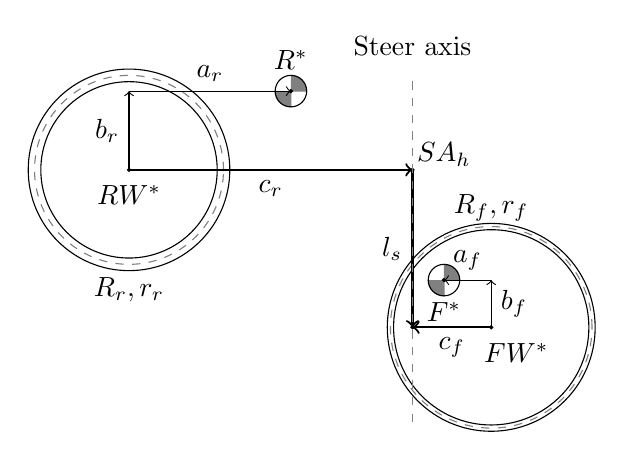
\begin{tikzpicture}[scale=4]
    %% Define constants
    \def\Rr{0.30cm}
    \def\Rf{0.32cm}
    \def\rr{0.02cm}
    \def\rf{0.01cm}
    \def\ar{0.514cm}
    \def\af{-0.15cm}
    \def\br{-0.25cm}
    \def\bf{-0.15cm}
    \def\cr{0.9cm}
    \def\cf{-0.25cm}
    \def\ls{0.5cm}
    \def\cmr{0.05cm}
    %% Locate important points
    \coordinate (RWO) at (0, 0);
    \coordinate (SAH) at ($(RWO) + (\cr, 0)$);
    \coordinate (SAF) at ($(SAH) - (0, \ls)$);
    \coordinate (FWO) at ($(SAF) - (\cf, 0)$);
    \coordinate (RO) at ($(RWO) + (\ar, -\br)$);
    \coordinate (FO) at ($(FWO) + (\af, -\bf)$);
    %% Draw important parts
    \node at ($(RWO) + (0,-.08cm)$) {$RW^*$};
    \node at ($(FWO) + (0.08cm,-.08cm)$) {$FW^*$};
    \node at ($(RO) + (0,.1cm)$) {$R^*$};
    \node at ($(FO) + (0,-.1cm)$) {$F^*$};
    \draw[draw=gray,dashed] (RWO) circle (\Rr);
    \draw[draw=gray,dashed] (FWO) circle (\Rf);
    \draw (RWO) circle (\Rr-\rr);
    \draw (FWO) circle (\Rf-\rf);
    \draw (RWO) circle (\Rr+\rr);
    \draw (FWO) circle (\Rf+\rf);
    \draw (270:\Rr+\rr+\rr+\rr+\rr) node {$R_r, r_r$};
    \draw (FWO) ++(90:\Rf+\rf+\rf+\rf+\rf+\rf+\rf) node {$R_f, r_f$};
    \draw[->,thick] (RWO) -- node[below] {$c_r$} (SAH);
    \draw[->,thick] (SAH) -- node[left] {$l_s$} (SAF);
    \draw[->,thick] (FWO) -- node[below] {$c_f$} (SAF);
    \filldraw[fill=gray,draw=gray] (RO) -- ++(\cmr, 0) arc (0:90:\cmr);
    \filldraw[fill=gray,draw=gray] (RO) -- ++(0, -\cmr) arc (270:180:\cmr);
    \draw(RO) circle (\cmr);
    \filldraw[fill=gray,draw=gray] (FO) -- ++(\cmr, 0) arc (0:90:\cmr);
    \filldraw[fill=gray,draw=gray] (FO) -- ++(0, -\cmr) arc (270:180:\cmr);
    \draw(FO) circle (\cmr);
    \draw[->] (RWO) -- node[left] {$b_r$} ++(0, -\br);
    \draw[->] ++($(RWO) + (0, -\br)$) -- node[auto] {$a_r$} ++(\ar, 0);
    \draw[->] (FWO) -- node[right] {$b_f$} ++(0, -\bf);
    \draw[->] ++($(FWO) + (0, -\bf)$) -- node[above] {$a_f$} ++(\af, 0);
    % Draw dots at center of wheels
    \filldraw (RWO) circle (.005cm);
    \filldraw (FWO) circle (.005cm);
    \filldraw (SAH) circle (.005cm);
    \filldraw (SAF) circle (.005cm);
    \filldraw (RO) circle (.005cm);
    \filldraw (FO) circle (.005cm);
    \coordinate (sa_label) at ($(SAH) + (0, .3cm)$);
    \coordinate (sah_label) at ($(SAH) + (.1cm, -.05cm)$);
    \draw[dashed,draw=gray] ($(SAF) + (0, -.3cm)$) -- (sa_label);
    \node[label=above:Steer axis] at (sa_label) {};
    \node[label=$SA_h$] at (sah_label) {};
  \end{tikzpicture}
  \caption[Bicycle geometric parameters.]{Bicycle geometric parameters. Not
    shown are the $X$ and $Z$ the gyrostat carriers which point to the right
    and down, respectively. As drawn, $b_r$, $a_f$, $b_f$, and $c_f$ are all
    negative; this is typical for traditional bicycles. Note that each
    parameter is defined without reference to the configuration of the bicycle.
    The head of the steer axis $SA_h$ is the point on top the steer axis and
    the foot of the steer axis $SA_f$ (not pictured) is the point on the bottom
    of the steer axis, both of which are fixed with respect to the gyrostat
    carriers $R$ and $F$.}
\label{model:fig:bicycle}
\end{figure}

Measuring the 23 (21 if the wheels are assumed to be knife edged) parameters
for a real bicycle is very similar to the procedure described
in~\cite{Moore2010b} except fewer measurements are needed. Instead of
determining the mass, mass center locations, and mass distribution of four
individual bodies, equivalent properties of only two cylindrical gyrostats need
to be measured. Practically speaking, this means only two masses need to be
measured (instead of four), the mass center locations and gyrostat inertia
measurements should be performed with the rear wheel and frame (front wheel and
fork) rigidly connected (i.e., wheel unable to spin), and the wheel moment of
inertia about an axis in the wheel plane needn't be measured (the wheel spin
inertia still does need to be measured, however). The time and energy savings
of the experimenter is fairly minor, however, the measurement of the fork
inertia can be problematic if the torsional pendulum stiffness is such that the
oscillations frequency are relatively high; by measuring the inertia of the
fork and wheel together, this is issue is mitigated to some degree. An
alternative method is to measure the exact parameters as described
in~\cite{Moore2010b}, and convert them to the gyrostat parameters as described
in \autoref{model:parameter_conversion}.

%The rear wheel is modelled as a rigid torus and is completely characterized by
%5 constant parameters: the major and minor radii, the mass, and two moments of
%inertia (one about the axis of symmetry, the other about any line in the wheel
%plane). The rear frame is modelled as a rigid body with unspecified geometry
%other than the spin axis of the wheel and steer axis which connects it to the
%fork. It is assumed that the two axes are perpendicular, that the frame is
%inertially symmetric about the plane perpendicular to the wheel spin axis, and
%that the steer axis lies in this symmetry plane. The bicycle frame is equipped
%with a dextral set of unit vectors: $\bs{r}_x, \bs{r}_y, \bs{r}_z=\bs{r}_x
%\times \bs{r}_y$ with $\bs{r}_y$ parallel the wheel axis and $\bs{r}_z$
%parallel to the steer axis. As described, the rear frame is completely
%characterized by 8 parameters: one distance between the wheel and steer axes as
%measured in the symmetry plane along a line perpendicular to the steer axis,
%two distances between the wheel spin axis and the mass center in the symmetry
%plane, the mass, and four central inertia scalars ($\bs{r}_x$ and $\bs{r}_z$
%are not assumed to be principal axes). If the rear wheel plane symmetry is
%constrained to lie in the bicycle symmetry plane, 13 parameters to completely
%describe these two bodies. Treated together, we can compute the combined mass,
%center of mass location (relative to the wheel axis), and the combined inertia
%about the center of mass. The combined mass and combined inertia represent 6
%unique scalar quantities as opposed to the 8 when the two bodies are considered
%separately. By describing the rear frame and rear wheel in terms of these
%combined parameters rather than the parameters intrinsic to each individual
%body, we use 2 fewer parameters. The same arguments apply to the  front fork
%and front wheel (replacing $\bs{r}_x, \bs{r}_y, \bs{r}_z$ with $\bs{f}_x,
%\bs{f}_y, \bs{f}_z$, respectively). With one final parameter describing the
%distance along the steer axis between the two bicycle frame and fork, we
%completely describe the bicycle with 23 parameters (11+11+1=23). See figure
%XXX.

\subsection{Parameter conversion}\label{model:parameter_conversion}
If the bicycle model in~\cite{Meijaard2007} is extended to use toroidal wheels
(as opposed to knife edged), and all Meijaard parameters remain otherwise
unchanged, a total of 27 parameters describe the bicycle model.  The two extra
parameters are the rear and front wheel minor radii, which we denote with
$t_\text{R}$ and $t_\text{F}$, respectively. The mapping from this 27
dimensional parameter space to the 23 dimensional gyrostat parameter space is
surjective -- distinct choices of Meijaard parameters can yield identical
gyrostat parameters (and hence identical dynamics). The practical implication
of this is that given a set of gyrostat parameters, it is not generally
possible to determine a unique set of the Meijaard parameters. This should not
be surprising given that it can be shown with dimensional analysis that the
minimal parameter space (assuming $t_\text{R}=t_\text{F}=0$) is only 9
dimensional~\cite{Sharp2008} (presumably it would be 11 dimensional if
$t_\text{R}$ and $t_\text{F}$ are included, though this has not been
verified).

In the equations that follow, the symbols used for the parameters presented
in~\cite{Meijaard2007} are on the right side of the equality, while the symbols
used to describe the gyrostat parameters are on the left of the equality. Some
parameters have very similar symbols but should not be confused as being the
same (i.e., $m_\text{f} \ne m_R$). Of the 23 gyrostat parameters, the following
6 have identical counterparts in the Meijaard parameters
\begin{align}
  J_r &= I_{\text{R}yy} \\
  R_r &= r_\text{R} \\
  r_r &= t_\text{R}\\
  J_f &= I_{\text{F}yy} \\
  R_f &= r_\text{F} \\
  r_f &= t_\text{F}
\end{align}
The rear and front gyrostat masses are trivially related
\begin{align}
  m_r &= m_\text{B} + m_\text{R} \\
  m_f &= m_\text{H} + m_\text{F}
\end{align}
With $s_\lambda=\sin\lambda$, $c_\lambda=\cos\lambda$, the mass center locations are related as
\begin{align}
a_r &= \frac{m_\text{B}}{m_\text{B} + m_\text{R}} \left(c_{\lambda} x_\text{B}
- s_{\lambda} \left(r_\text{R} + t_\text{R} + z_\text{B}\right)\right) \\
b_r &= \frac{m_\text{B}}{m_\text{B} + m_\text{R}} \left(c_{\lambda}
\left(r_\text{R} + t_\text{R} + z_\text{B}\right) + s_{\lambda} x_\text{B}\right) \\
a_f &= - \frac{m_\text{H}}{m_\text{F} + m_\text{H}} \left(c_{\lambda} \left(w -
x_\text{H}\right) + s_{\lambda} \left(r_\text{F} + t_\text{F} + z_\text{H}\right)\right) \\
b_f &= \frac{m_\text{H}}{m_\text{F} + m_\text{H}} \left(c_{\lambda}
\left(r_\text{F} + t_\text{F} + z_\text{H}\right) - s_{\lambda} \left(w -
x_\text{H}\right)\right)
\end{align}
The three parameters which describe the perpendicular distance of the wheel centers from the
steer axis, and the distance between these perpendicular lines are
\begin{align}
c_r &= c_{\lambda} \left(c + w\right) - s_{\lambda} \left(r_\text{R} +
t_{R}\right) \\
c_f &= c_{\lambda} c - s_{\lambda} \left(r_\text{F} + t_\text{F}\right) \\
l_s &= - c_{\lambda} \left(r_\text{F} - r_\text{R} + t_\text{F} - t_\text{R}\right) + s_{\lambda} w
\end{align}
The central inertia scalars of the two gyrostats in terms of the Meijaard
parameters are
\begin{align}
I_{rxx} &=
I_{\text{R}xx} +
c_\lambda^2 I_{\text{B}xx} - 2 s_\lambda c_\lambda I_{\text{B}xz} + s_\lambda^2
I_{\text{B}zz} \notag\\
& + \frac{m_\text{R} m_\text{B}}{\left(m_\text{R} +
m_\text{B}\right)}\left(s_\lambda x_\text{B} + c_\lambda \left(r_\text{R} +
t_\text{R} + z_\text{B}\right)\right)^2 \\
%
I_{ryy} &= I_{\text{R}yy} + I_{\text{B}yy} \notag\\
& + \frac{m_\text{R} m_\text{B}}{\left(m_\text{R} + m_\text{B}\right)}
\left(x_\text{B}^2 + \left(r_\text{R} + t_\text{R} + z_\text{B}\right)^2
\right) \\
%
I_{rzz} &= I_{\text{R}xx} +
s_\lambda^2 I_{\text{B}xx} + 2 s_\lambda c_\lambda I_{\text{B}xz} + c_\lambda^2
I_{\text{B}zz} \notag\\
& + \frac{m_\text{R} m_\text{B}}{\left(m_\text{R} + m_\text{B}\right)}
\left(c_{\lambda} x_\text{B} - s_\lambda \left(r_\text{R} + t_\text{R} +
z_\text{B}\right)\right)^{2}\\
%
I_{rxz} &= \left(c_\lambda^2 - s_\lambda^2\right) I_{\text{B}xz}
+ s_\lambda c_\lambda \left(I_{\text{B}xx} - I_{\text{B}zz}\right) \notag\\
& - \frac{m_\text{B} m_\text{R}}{\left(m_\text{B} + m_\text{R}\right)}
\left(c_\lambda x_\text{B} - s_\lambda \left(r_\text{R} + t_\text{R} +
z_\text{B}\right)\right) \left(s_{\lambda} x_\text{B} + c_\lambda \left(r_\text{R} + t_\text{R} +
z_\text{B}\right)\right) \\
%
I_{fxx} &= I_{\text{F}xx} +
c_\lambda^2 I_{\text{H}xx} - 2 s_\lambda c_\lambda I_{\text{H}xz} + s_\lambda^2
I_{\text{H}zz} \notag\\
& + \frac{m_\text{H} m_\text{F}}{\left(m_\text{F} + m_\text{H}\right)} \left(- s_{\lambda} \left(w -
x_\text{H}\right) + c_{\lambda}
\left(r_\text{F} + t_\text{F} + z_\text{H}\right)\right)^{2}\\
%
I_{fyy} &= I_{\text{F}yy} + I_{\text{H}yy} \notag \\
& + \frac{m_\text{F} m_\text{H}}{\left(m_\text{F} + m_\text{H}\right)}
\left(\left(w - x_\text{H}\right)^2 + \left(r_\text{F} + t_\text{F} +
z_\text{H}\right)^2\right) \\
%
I_{fzz} &= I_{\text{F}xx} +
s_\lambda^2 I_{\text{H}xx} + 2 s_\lambda c_\lambda I_{\text{H}xz} + c_\lambda^2
I_{\text{H}zz} \notag\\
& + \frac{m_\text{F} m_\text{H}}{\left(m_\text{F} + m_\text{H}\right)} \left(c_{\lambda}
\left(w - x_\text{H}\right) + s_{\lambda} \left(r_\text{F} + t_\text{F} +
z_\text{H}\right)\right)^{2}\\
%
I_{fxz} &= \left(c_\lambda^2 - s_\lambda^2\right) I_{\text{H}xz}
+ s_\lambda c_\lambda \left(I_{\text{H}xx} - I_{\text{H}zz}\right) \notag\\
& + \frac{m_\text{F} m_\text{H}}{\left(m_\text{F} + m_\text{H}\right)}
\left(c_\lambda \left(w - x_\text{H}\right) + s_\lambda \left(r_\text{F} +
t_\text{F} + z_\text{H}\right)\right) \left(- s_{\lambda} \left(w -
x_\text{H}\right) + c_\lambda \left(r_\text{F} + t_\text{F} +
z_\text{H}\right)\right)
\end{align}
The numerical values of the benchmark parameter set presented
in~\cite{Meijaard2007} convert to the gyrostat parameters shown in
\autoref{model:table:parameters}.

\begin{table}[htbp]
  \centering
  \begin{tabular}{rccl}
    \toprule
    & {Rear gyrostat} & {Front gyrostat} & {Units} \\
    \midrule
    $I_{xx}$ &   7.684799791449106 &    0.4335379755311007  & \si{\kg\m\squared} \\
    $I_{yy}$ &   11.99931034482759 &    0.5746857142857142  & \si{\kg\m\squared} \\
    $I_{zz}$ &   5.315110553378478 &    0.1481477387546135  & \si{\kg\m\squared} \\
    $I_{xz}$ &   4.262158094617231 &  0.005332503757935524  & \si{\kg\m\squared} \\
         $J$ &                0.12 &                  0.28  & \si{\kg\m\squared} \\
         $m$ &                  87 &                     7  & \si{\kg}     \\
         $R$ &                 0.3 &                  0.35  & \si{\m}      \\
         $r$ &                   0 &                     0  & \si{\m}\\
         $a$ &  0.4599058376856177 & -0.003411905099535333  & \si{\m}\\
         $b$ & -0.4669419422355365 &   -0.2114010400161699  & \si{\m}\\
         $c$ &  0.9534570696121847 &   -0.0320714267276193  & \si{\m}\\
         $l_s$ & \multicolumn{2}{c}{0.2676445084476887} &  \si{\m} \\
  \bottomrule
  \end{tabular}
  \caption[Benchmark bicycle parameters converted to gyrostat
    parameters.]{Benchmark bicycle parameters converted to gyrostat parameters.
    Parameters shown to 15 or more decimal places are not exact.}
  \label{model:table:parameters}
\end{table}

\section{Kinematics} \label{model:kinematics}

Were the four bodies of the bicycle model to be disconnected and free to move
in an arbitrary manner, the system would have 24 degrees of freedom (4 bodies,
6 degrees of freedom per body). Accounting for the 3 revolute joints (wheel
axes and steer axis) reduces the number of degrees of freedom from 24 to 9
(each revolute joint removes 5 degrees of freedom). Requiring the lowest point
of the rear wheel and front wheel to touch the horizontal ground plane removes
two further degrees of freedom, resulting in 7 configuration degrees of
freedom. A minimal choice of configuration variables is not practical (nor
generally possible for all configurations) due to the complexity of the
holonomic constraint (it is nonlinear and has multiple
roots)~\cite{Peterson2008a}.

The revolute joints and the requirement that the wheels make point contact with
the ground plane are configuration (holonomic) constraints. Without any further
restrictions regarding the wheel contact with the ground, the system has 7
velocity degrees of freedom as well. If simulation or stability analysis of
such a model is desired, a model for the forces at the wheel contact points is
needed. If it is instead assumed that the wheels roll without slip (said
another way, the wheel contact forces are whatever is necessary to prevent
slip), 4 more degrees of freedom are removed (2 from each no-slip assumption),
yielding a system with 3 velocity degrees of freedom. The no-slip assumptions
do not constrain the configuration in any way, so the accessible configuration
space remains 7 dimensional, but the dimension of the accessible velocity space
is reduced from 7 to 3 under the assumption of no-slip.  The remainder of this
chapter assumes that the wheels do not slip relative to the ground (and hence
the system has 3 velocity degrees of freedom).

A wise choice of generalized coordinates can result in a reduction of the
number of configuration constraints that need to be solved. A familiar example
is the pendulum: using $x$ and $y$ to locate the pendulum mass and deriving the
equations of motion in terms of $x$ and $y$ (and their derivatives) requires
enforcing the constraint $l - \sqrt{x^2 + y^2} = 0$. This choice is ill advised
and best avoided in favor of choosing a single generalized coordinate (i.e.,
the pendulum angle $\theta$) which implicitly satisfies the length constraint.
It is generally in the interest of the analyst to introduce the minimal
number of coordinates possible so that needless configuration constraint
equations are avoided.

Similarly, a wise choice of generalized speeds can reduce or eliminate the
number of velocity constraints that need to be solved. A familiar example of
this is the rolling disk: only three generalized speeds are needed to fully
describe the angular velocity of the disk \textit{and} the velocity of the disk
mass center, and therefore no velocity constraint equations need to be solved
explicitly to obtain the dynamic equations. If instead one introduces six
generalized speeds (e.g., three for the disk angular velocity and three for the
velocity of the mass center), three scalar constraint equations must be
satisfied and hence only three of the generalized speeds can be chosen
independently. Which to choose as independent in the case of the rolling disk
is fairly obvious, but for more complicated systems this is not generally the
case and care must be taken\cite{Reckdahl1996}. Just as in the case for
generalized coordinates, it is generally in the interest of the analyst to
introduce the minimal number of generalized speeds as possible so that needless
velocity constraint equations are avoided.

With this wisdom in mind, we describe the configuration and velocity of the
bicycle with 8 generalized coordinates and 6 speeds. This choice results in 1
configuration constraint and 3 velocity constraints. With the exception of
frame pitch the coordinates used are identical to the coordinates presented
in~\cite{Meijaard2007}.

Let $X_NY_NZ_N$ be a set of mutually perpendicular axes fixed in a Newtonian
frame $N$, intersecting at the inertial origin $N^*$, with the positive $Z$
axis pointing down into the ground plane and parallel to the local
gravitational field. Let $\uv{n}{x}, \uv{n}{y}, \uv{n}{z}$ be a set of dextral
unit vectors aligned with $X, Y, Z,$ respectively. Similarly let the rear
gyrostat carrier $R$ and the front gyrostat carrier $F$ be equipped with axes
$X_RY_RZ_R$ and $X_FY_FZ_F$, respectively, each intersecting at their
respective gyrostat mass centers $R^*$ and $F^*$. Let $Z_R \parallel Z_F$ also
be parallel to the steer axis $SA$. Further, let the wheel spin axis of each
carrier be parallel to $Y_R$ and $Y_F$, respectively. Let $\uv{r}{x},
\uv{r}{y}, \uv{r}{z}$ be a set of dextral unit vectors aligned with $X_R, Y_R,
Z_R$, respectively, and similarly let $\uv{f}{x}, \uv{f}{y}, \uv{f}{z}$ be a
set of dextral unit vectors aligned with $X_F, Y_F, Z_F$, respectively.

To orient $R$ relative to $N$, first align $X_RY_RZ_R$ with $X_NY_NZ_N$ then
apply a sequence of body fixed $ZXY$ rotations: yaw $\psi$, lean $\phi$, and
pitch $\theta$. The two intermediate frames in the sequence of rotations are
the instantaneous yaw frame $Y$ and the instantaneous lean frame $L$. To orient
$F$ relative to $R$, first align $X_FY_FZ_F$ with $X_RY_RZ_R$ (and note that
$Z_R \parallel SA \parallel Z_F$, then a apply a right handed rotation to $F$
about SA by steer angle $\delta$. Finally, to orient the wheels relative to
their respective carrier, apply simple right handed rotations of the wheel
relative to the carrier by angles $\theta_r$ and $\theta_f$, respectively.
These six rotations completely define the orientation of all frames relative to
each other. 

The position of the gyrostat mass centers relative to the wheel centers is
defined by the choice of parameters $a_r, b_r, a_f, b_f$ (see
\autoref{model:fig:bicycle}). The from the rear wheel center $RW^*$ to the rear
gyrostat mass center $R^*$ is $\bs{r}^{RW^*R^*} = a_r \uv{r}{x} + b_r
\uv{r}{z}$; similarly the position from the front wheel center $FW^*$ to the
front gyrostat mass center $F^*$ is $\bs{r}^{FW^*F^*} = a_f \uv{f}{x} + b_f
\uv{f}{z}$. The position from the rear wheel center to the front wheel center
is $\bs{r}^{RW^*FW^*} = c_r \uv{r}{x} + l_s \uv{r}{z} - c_f \uv{f}{x}$. We
introduce the final two generalized coordinates $x$ and $y$, to locate the rear
wheel ground contact $P$, The position from the inertial origin $N^*$ to the
rear wheel ground contact $P$ is $\bs{r}^{N^*RW^*} = x \uv{n}{x} + y
\uv{n}{y}$. The position from $P$ to the rear wheel center $RW^*$ is as
$\bs{r}^{PRW^*} = - r_r \uv{y}{z} - R_r \uv{l}{z}$ ($\uv{y}{z}$ is the downwards
vertical unit vector of the instantaneous yaw frame $Y$, and $\uv{l}{z}$ is the
result of rotating $\uv{y}{z}$ be lean angle $\phi$).  The remaining point is
the front wheel ground contact $Q$. To define the position from the front wheel
center $FW^*$ to $Q$ we introduce the unit vector
\begin{align}
  \uv{g}{z} &= \frac{\uv{y}{z} - (\uv{f}{y} \cdot \uv{y}{z})
  \uv{f}{y}}{|\uv{y}{z} - (\uv{f}{y} \cdot \uv{y}{z})
  \uv{f}{y}|}
\end{align}
which is the projection of the downwards vertical vector $\uv{y}{z}=\uv{n}{z}$
onto the front wheel plane ($\uv{f}{y}$ is normal to the front wheel plane).
The position from the front wheel center is now be simply written as
$\bs{r}^{FW^*Q} = R_f \uv{g}{z} + r_f \uv{y}{z}$. The eight generalized
coordinates used to fully orient the four bodies and locate each of the mass
centers summarized in \autoref{model:tab:coordinates}.

\begin{table}[htbp]
  \centering
  \begin{tabular}{ccc}
    \toprule
    Coordinate & Description & Units \\
    \midrule
    $\psi$ & Bicycle frame yaw angle & \si{\radian} \\
    $\phi$ & Bicycle frame lean angle & \si{\radian} \\
    $\theta$ & Bicycle frame pitch angle  & \si{\radian} \\
    $\delta$ & Steer angle & \si{\radian} \\
    $\theta_r$ & Rear wheel angle & \si{\radian} \\
    $\theta_f$ & Front wheel angle & \si{\radian} \\
    $x$ & Rear wheel contact $P$ $X_N$ measure number & \si{\m} \\
    $y$ & Rear wheel contact $P$ $Y_N$ measure number & \si{\m} \\
    \bottomrule
  \end{tabular}
  \caption[Bicycle generalized coordinates.]{Bicycle generalized coordinates.
    In the upright $\phi=0$ zero steer $\delta=0$ configuration, the pitch
    angle $\theta$ is equal to the steer axis tilt $\lambda$ of the benchmark
    parameter set. This is in contrast to the pitch $\theta_{\text{B}}$ defined
    in~\cite{Meijaard2007}, which is zero in the same configuration. The two
    pitch coordinates are related as $\theta = \theta_{\text{B}} + \lambda$;
    the other 7 coordinates are identical.}
  \label{model:tab:coordinates}
\end{table}

In order to maintain contact with the ground plane the following configuration
constraint must be satisfied
\begin{align}
  \bs{r}^{PQ} \cdot \uv{y}{z} &= 0
\end{align}
which is the mathematical statement that the lowest point of the front wheel
must lie in the ground plane. The dot product on the left hand side depends on
the three coordinates lean $\phi$, pitch $\theta$, steer $\delta$, and seven
geometric parameters (the wheel radii $R_r, r_r, R_f, r_f$, and the distances
$c_r, c_f$, and $l_s$). We introduce a vector $q\in\mathbb{R}^3$ for the three
coordinates and a vector $p\in\mathbb{R}^7$ for the parameters involved in this
constraint
\begin{align}
  q &\triangleq \left[\phi, \theta, \delta\right]\label{model:q_min}\\
  p &\triangleq \left[R_r, r_r, R_f, r_f, c_r, c_f, l_s\right]
  \label{model:constraint_parameters}
\end{align}
we can write the configuration constraint concisely as
\begin{align}
  f_c(q, p) &= 0
  \label{model:f_c}
\end{align}
where $f_c : \mathbb{R}^3 \times \mathbb{R}^7 \mapsto \mathbb{R}$.  The three
elements of $q$ cannot be varied independent and most often the pitch $\theta$
is selected to be a dependent coordinate.

The angular velocity of the four bodies and the velocity of the gyrostat mass
centers can be defined with only six generalized speeds. These six generalized
speeds are defined as follows
\begin{align}
  u_{1} &\triangleq \dot{\psi} \\
  u_{2} &\triangleq \dot{\phi} \\
  u_{3} &\triangleq \dot{\theta} \\
  u_{4} &\triangleq \dot{\delta} \\
  u_{5} &\triangleq \dot{\theta}_r \\
  u_{6} &\triangleq \dot{\theta}_f
\end{align}
The angular velocity of the four bodies relative to the $N$ is fully
established by the following relations
\begin{align}
  {}^{N}\bs{\omega}^{R} &= u_1 \uv{y}{z} + u_2 \uv{l}{x} + u_3\uv{r}{y} \\
  {}^{R}\bs{\omega}^{F} &= u_4 \uv{r}{z} = u_4 \uv{f}{z} \\
  {}^{R}\bs{\omega}^{RW} &= u_5 \uv{r}{y} \\
  {}^{F}\bs{\omega}^{FW} &= u_6 \uv{f}{y}
\end{align}
The velocity of the gyrostat mass centers $R^*$ and $F^*$, relative to $N$, are
obtained by assuming the wheel contacts $P$ and $Q$ do not slip relative to the
ground plane (i.e., ${}^{N}\bs{v}^{P} = {}^{N}\bs{v}^{Q} = \bs{0}$) and applying the two
point velocity theorem to form the velocity of the wheel centers as follows
\begin{align}
  {}^{N}\bs{v}^{RW^*} &= {}^{N}\bs{\omega}^{RW} \times \bs{r}^{PRW^*} \\
  {}^{N}\bs{v}^{R^*} &= {}^{N}\bs{v}^{RW^*} + {}^{N}\bs{\omega}^{R} \times \bs{r}^{RW^*R^*} \\
  {}^{N}\bs{v}^{FW^*} &= {}^{N}\bs{\omega}^{FW} \times \bs{r}^{QFW^*} \\
  {}^{N}\bs{v}^{F^*} &= {}^{N}\bs{v}^{FW^*} + {}^{N}\bs{\omega}^{F} \times \bs{r}^{FW^*F^*}
\end{align}
The velocity constraints are obtained by equating the velocity of a point on
the steer axis obtained in two separate, but equally valid ways. Because the
steer axis is fixed in both gyrostat carriers, the velocity of this point
obtained with the two approaches must be equal. The velocity of the head of the
steer axis $SA_h$ (see \autoref{model:fig:bicycle}) is obtained by working from
the rear contact $P$ through the rear wheel $RW$ and bicycle frame $R$
\begin{align}
  {}^{N}\bs{v}^{SA_h}_r &= {}^{N}\bs{v}^{RW^*} + {}^{N}\bs{\omega}^{R} \times \bs{r}^{RW^*SA_h}
\end{align}
while working from the front contact point $Q$ through the front wheel $FW$ and
fork $F$ gives
\begin{align}
  {}^{N}\bs{v}^{SA_h}_f &= {}^{N}\bs{v}^{FW^*} + {}^{N}\bs{\omega}^{F} \times \bs{r}^{FW^*SA_h}
\end{align}
where $_r$ and $_f$ denote which set of bodies were used to when obtaining the
velocity of $SA_h$. The velocity constraints in vector form are then
\begin{align}
  {}^{N}\bs{v}^{SA_h}_r - {}^{N}\bs{v}^{SA_h}_f &= \bs{0}
  \label{model:eq:f_v_vec}
\end{align}
Taking the dot product of \autoref{model:eq:f_v_vec} with any three
perpendicular vectors (i.e., $\uv{r}{x}, \uv{r}{y}, \uv{r}{z}$), yields three
scalar equations which are linear in the 6 generalized speeds $u_1 \dots u_6$.
These three scalar equations can be written in matrix form as
\begin{align}
  B(q, p) u &= 0
  \label{model:eq:f_v_matrix}
\end{align}
where $B\in\mathbb{R}^{3 \times 6}$, $u\in\mathbb{R}^{6 \times 1}$ and $p$ and
$q$ are defined in \autoref{model:q_min} and
\autoref{model:constraint_parameters}, respectively. By choosing three of the
six generalized speeds as independent, it is possible to solve
\autoref{model:eq:f_v_matrix} for the other three (dependent) speeds.
Typically, lean rate $\dot{\phi} = u_2$, steer rate $\dot{\delta} = u_4$, and
one of the wheel rates ($\dot{\theta}_r = u_5$ or $\dot{\theta}_f = u_6$) are
chosen to be the independent speeds.


\section{Dynamics}
A large portion of the complexity of the bicycle dynamic equations is caused by
the velocity constraints. However, careful book keeping of the kinematic
quantities using a symbolic computer algebra system such as SymPy~\cite{SymPy}
makes forming the dynamic equations much less tedious. The kinematics as
presented in \autoref{model:kinematics} were programmed into a Python script
which derives the dynamic equations of motion using Kane's
method~\cite{Kane1985}. The symbolic equations were exported to C++ files which
were then compiled into a software library~\cite{libbicycle} which provides
efficient and convenient functionality to compute eigenvalues, calculate ground
reaction forces, compute linearized system dynamics matrices, and perform
numerical simulation. This library was used to compute all the system dynamics
matrices used in the design of the control system presented in
\autoref{chapter4}.



\printbibliography[section=2,heading=subbibliography]
\chapter{Linearization of equations of motion of constrained multibody systems}
\label{chapter3}
\section{Introduction}
\label{sec:intro}

Many common dynamic mechanical systems have configuration or velocity
constraints.  Analyses of such systems often require linearized forms of the
motion equations.  To address this issue, we developed a procedure for
organizing the constraint and motion equations and their subsequent
linearization.  This procedure was specifically developed for equations of
motion generated by Kane's method, but is compatible with any method as long as
the following are true: only ordinary differential equations are required to
describe the system, and independent and dependent states remain in the final
equations (i.e. no DAE's, no substitution of variables).  Following a brief
review of Kane's method and the structure of the equations it generates, we
present the procedure to symbolically linearize the nonlinear motion equations
of constrained multibody systems, and illustrate it with the familiar example
of the rolling disk.

Design of linear state feedback controllers and first order stability analysis
of equilibria are two of the most common uses of multibody system dynamics
models. Both of these uses require linearized equations of motion. For
unconstrained systems, obtaining the linearized equations of motion is as
simple as arranging the equations of motion in first order form ($\dot{x} =
f(x, t)$) and evaluating the Jacobian of the right hand side function, with
respect to the states, evaluated at the equilibria point of interest.  However,
when the system in questions has constraints, i.e., not all the states are
independent, this process is not as straightforward.

For a system system with constraints, Kane's dynamical
equations~\cite{Kane1985} are first order ODE's (in the generalized speeds)
which include both the independent and dependent states (assuming the
dependents states have not been algebraically eliminated). The kinematical and
dynamical differential equations can be solved for the time derivatives of the
generalized coordinates and generalized speeds, respectively. Taken together,
it is tempting to think that this system of first order differential equations
could be linearized in the same fashion as an unconstrained system.
Unfortunately, this is not the case.  Linearizing these equations in the same
manner as one would for an unconstrained system (by directly computing the
Jacobian) is incorrect and will yield incorrect linearized equations (and
subsequently incorrect eigenvalues, in the case of a stability analysis). We
illustrate this by means of a familiar example, the rolling disk, formulated
with a non-traditional set of coordinates and generalized speeds which are not
all independent. We provide a systematic method to correctly generate the
linear equations of motion for constrained systems which have been found using
Kane's method (or any other method which results in equations with the same
form). We apply this method to the rolling disk example to illustrate that it
yields eigenvalues that match previously published results.

We consider three types of constraints: configuration, velocity, and
acceleration. Configuration constraints limit the location or orientation of
parts of the system, relative to the external world or other parts of the
system. Velocity constraints limit the speeds at which the configuration can
change, either from configuration constraints (through time differentiation) or
independent application. Velocity constraints most often appear in systems
where there is rolling without slip or there are closed kinematic loops. In the
context of this chapter, acceleration constraints arise either from time
differentiated velocity constraints or similar kinematic considerations.

% TODO: Improve literature review.
Bottema appears to be the first author to have shown that special
considerations are needed for linearizing nonholonomic
systems~\cite{Bottema1949}. While other authors have examined linearization of
nonholonomic systems, we have found that most techniques are not directly
applicable to equations formed using Kane's method, and while we do not doubt
that they \textit{could} be applied correctly, the details of how to do so, as
far as the authors are aware, have not been explicitly presented. Kang et
al.~\cite{Kang2003} and Negrut and Ortiz~\cite{Negrut2006} have both explored
linearization, but these methods have been developed for equations of motion
found using Lagrange's method, which contain Lagrange multipliers (which are
not present in equations of motion generated from Kane's method). Further, both
of these papers lack a discussion of basic concepts such as how many quantities
are independent, and in the case of eigenvalue computation, how many
eigenvalues should be present. Minaker and Rieveley~\cite{Minaker2010} and
Schwab and Meijaard~\cite{Schwab2003} both have developed techniques for
generating equations of motion (and linear forms thereof) using Lagrange's
method; the work of Schwab and Meijaard can be applied symbolically while
Minaker and Reiveley's approach is numeric in nature. Neither discuss the
choice of generalized speeds as in Kane's method: both form the equations of
motion in terms of second time derivatives of the coordinates.  Further,
neither of these works address constraints which cannot be eliminated (i.e.,
nonlinear configuration constraints), nor do they address what approach should
be taken when a single choice of dependent states may not suffice. While Neuman
presents a symbolic (as opposed to numeric) formulation for linearization of
the Q-matrix formulation of the Lagrangian~\cite{Neuman1984}, his work makes no
mention of constrained systems and attempts to contact the author regarding the
software (algebraic robot modeler -- Arm) as well as internet searches for the
software have been fruitless.

The goal of this chapter is to definitively establish how the first time
derivative of all coordinates and speeds (independent and dependent)
depend, to first order, upon a selection of independent coordinates and
independent speeds, for an arbitrary point of linearization. We demonstrate how
a reduced portion of these linearized equations can be used to perform standard
stability analysis (i.e., for control system design or linear stability
analysis). The formalism presented here is generic enough to cover most
examples of time-varying constrained multibody systems with arbitrary external
inputs and arbitrary specified quantities.  The procedure was created for
systems whose equations of motion have been derived with Kane's method.
Although also applicable to dynamic system equations formulated using other
methods, it is restricted to systems which can be completely described by a set
of ODE's (i.e., DAE's needn't be solved).

We begin with a review of Kane's method for generating equations of motion is
reviewed first, in order to properly orient the reader to the format and some
of the qualities of the generated equations. Next, we apply Kane's method to
generate the equations of motion for the rolling disk, but we purposefully
introduce a dependent coordinate and three dependent speeds in the formulation.
The need for a different linearization technique is demonstrated with this
example. In response to this need, we present the newly developed linearization
procedure and its derivation. This new linearization procedure is applied the
same rolling disk example to illustrate its validity and an example of its
application. Finally, we discuss other details and nuances of the procedure and
its use, as well as directions for future work.

\section{Kane's method, briefly}
\label{sec:kane_method}
To familiarize the reader with Kane's method, some concepts relating to its use
will be described.  The first is the use of generalized speeds in addition to
generalized coordinates.  The second concept is in how these generalized speeds
can be used to project permissible motions of the system, and how this removes
the need to consider non-contributing (internal constraint) forces.  Then, the
mathematical steps required to use Kane's method are shown and described.

When using Lagrange's method, generalized coordinates are used to describe the
configuration of a system while the time derivatives of the generalized
coordinates describe the velocities of a system.  Kane's method allows for the
velocities of a system to be written in terms of generalized speeds, which are
not required to be the time derivatives of coordinates (although such a
definition is permitted).

The benefit of choosing generalized speeds to be other than simply the
derivatives of the corresponding generalized coordinates can be seen in the
following example. If the orientation of a rigid body were to be described
using using Euler parameters or quaternions as coordinates, its angular
velocity in terms of time derivatives of those coordinates is relatively
complicated; it also requires a velocity constraint. Using generalized speeds
allows for the angular velocity to be expressed more simply as
\begin{align}
\label{eq:ex1}
{^N}\bs{\omega}^B = \omega_1 \uv{b}{1} + \omega_2 \uv{u}{2} + \omega_3 \uv{b}{3}
\end{align}
or, the angular velocity of rigid body $B$ in the reference frame $N$ is the
defined as the sum of three generalized--speed basis--vector products.
The derivatives of these generalized speeds will appear in the equations
of motion, rather than the twice time differentiated generalized coordinates
($\ddot{{q}}$'s).

A drawback of allowing such definitions can be seen when formulating the
kinematic differential equations, which relate the rate of change of the
generalized coordinates to the generalized speeds. These equations become more
complicated (in comparison to $\dot{q}_i = u_i$), but this is usually offset by
the significantly simpler dynamical equations of motion~\cite{Mitiguy1996}.

Use and understanding of Kane's method requires the use and understanding of
partial velocities and partial angular velocities. These are simply the
partial derivatives of the (angular) velocity vectors with respect to the
generalized speeds. For example, for the angular velocity in equation
(\ref{eq:ex1}), the partial angular velocities of body $B$ in reference frame
$N$ are
\[
  {^N}\bs{\omega}^B_{\omega_1} = \uv{b}{1} \quad \quad
  {^N}\bs{\omega}^B_{\omega_2} = \uv{b}{2} \quad \quad
  {^N}\bs{\omega}^B_{\omega_3} = \uv{b}{3}
\]
and it can be seen that the partial velocities represent the direction of
motion associated with each generalized speed. The geometric interpretations of
these partial (angular) velocities are discussed at length by
Lesser~\cite{Lesser1992}.

Taking the dot product of each partial velocity and both sides of Newton's
second law, $\bs{F}=m\bs{a}$ (or the rotational equivalent), only terms that
are parallel to the partial velocities remain; one scalar equation is generated
for each generalized speed. An important byproduct is that internal constraint forces
(non-contributing forces) imposed by objects such as pin or sliding joints no
longer need to be considered. The reason for this is that partial velocities
are \textit{by construction} perpendicular to forces of constraint. Constraint
forces can be included in the formulation, but will not appear in the final
equations of motion because of this very desirable property.

In summary, Kane's method allows for velocities to be defined in terms of
generalized speeds, allowing for simpler velocity expressions.  The dot product
of each partial velocity (the direction of motion associated with each
generalized speed) with Newton's second law (or Euler's equations) removes all
terms which are not related to the rate of change of each generalized speed.
This generally results in simple equations of motion, which are easier to form.

The mathematical formalism for applying Kane's method to multibody systems
follows. Consider a system composed of particles $P_1,...,P_h$, rigid bodies
$B_1,...,B_g$, with points of force application $Q_1,...,Q_k$, and reference
frames of torque application $E_1,...,E_c$, all defined relative to the
inertial reference frame $N$. This system has generalized coordinates
$q_1,...,q_n$ and generalized speeds $u_1,...,u_o$. Additionally, there are $l$
configuration constraints and $m$ velocity constraints.

In order to properly apply Kane's method, the velocities of each component in
the system need to be written as linear combinations of the generalized speeds.
The translational velocity of the particles are
\begin{align}
\label{eq:particle_translational}
{^N}\bs{v}^{P_i} = \sum^o_{j=1} {^N}\bs{v}^{P_i}_{u_j} u_j + {^N}\bs{v}^{P_i}_t
\quad \quad i=1,...,g
\end{align}
while the translational velocity of rigid body mass centers are
\begin{align}
\label{eq:rb_translational}
{^N}\bs{v}^{B_i^*} = \sum_{j=1}^o {^N}\bs{v}^{B_i^*}_{u_j} u_j +
{^N}\bs{v}^{B_i^*}_t \quad \quad i=1,...,h
\end{align}
and finally the translational velocity of points which have applied forces are
\begin{align}
\label{eq:points_translational}
{^N}\bs{v}^{Q_i} = \sum_{j=1}^o {^N}\bs{v}^{Q_i}_{u_j} u_j + {^N}\bs{v}^{Q_i}_t
\quad \quad i=1,...,k
\end{align}
Next, the angular velocity of rigid bodies are
\begin{align}
\label{eq:rb_rotational_bodies}
{^N}\bs{\omega}^{B_i} = \sum_{j=1}^o {^N}\bs{\omega}^{B_i}_{u_j} u_j +
{^N}\bs{\omega}^{B_i}_t \quad \quad i=1,...,h
\end{align}
and the angular velocity of reference frames which have applied torques are
\begin{align}
\label{eq:rb_rotational_frames}
{^N}\bs{\omega}^{E_i} = \sum_{j=1}^o {^N}\bs{\omega}^{E_i}_{u_j} u_j +
{^N}\bs{\omega}^{E_i}_t \quad \quad i=1,...,c
\end{align}
In these equations, each term $\bs{v}_t$ or $\bs{\omega}_t$ represents a
velocity or angular velocity component which is a prescribed function of time,
and has no dependence on generalized speeds (e.g., a motor or crank driven at a
specified rate).

For this system, we consider configuration constraints of the form
\begin{align}
\label{eq:configuration_constraints}
f_c(q, t) = 0
\end{align}
where $q\in\mathbb{R}^n, t\in\mathbb{R}$, and $f_c : \mathbb{R}^n \times
\mathbb{R} \mapsto \mathbb{R}^l$.  The velocity constraints are taken to have
the form
\begin{align}
\label{eq:velocity_constraints}
f_v(q, u, t) = 0
\end{align}
where $u\in\mathbb{R}^o$, $f_v : \mathbb{R}^n \times \mathbb{R}^o \times
\mathbb{R} \mapsto \mathbb{R}^m$, and $f_v$ is linear in $u$.  It is important
that the velocity constraints include the time-differentiated configuration
constraints or equivalent constraints which produce the same behavior.
Furthermore, velocity constraints should be written such that generalized
speeds and coordinates appear, but $\dot{q}$ terms do not (i.e., they should be
eliminated by appealing to the kinematic differential equations). Finally,
acceleration constraints are typically time-differentiated velocity constraints
(or similarly formed from kinematic considerations) and are assumed to have the
form
\begin{align}
  \label{eq:acceleration_constraints}
  f_a(q, \dot{q}, u, \dot{u}, t) = 0
\end{align}
where $f_a : \mathbb{R}^n \times \mathbb{R}^n \times \mathbb{R}^o \times
\mathbb{R}^o \times \mathbb{R} \mapsto \mathbb{R}^m$. In contrast to the
velocity constraints, our formulation permits the acceleration constraints to
involve $\dot{q}$ terms, although eliminating them using by appealing to the
kinematic differential equations presents no problems. By assumption, the
velocity constraints are linear with respect to $u$, so we introduce
\begin{align}
\label{eq:constraint_B}
  B &\triangleq \nabla_u f_v (q, u, t)
\end{align}
which implies that $B : \mathbb{R}^n \times \mathbb{R} \mapsto \mathbb{R}^m
\times \mathbb{R}^o$, i.e, $B$ is an $m \times o$ matrix whose entries depend
on $q$ and $t$. The velocity constraint equations may now be written as
\begin{align}
\label{eq:constraint_Bu0}
B u + f_{vt}(q, t) &= 0
\end{align}
where $f_{vt} : \mathbb{R}^n \times \mathbb{R} \mapsto \mathbb{R}^m$ arises if
there are explicit time varying terms in the velocity constraints. These
typically arise from specified quantities whose dynamics are being ignored
(e.g., a motor spinning at constant speed).

With these definitions established, Kane's method can be applied. In vector
form, Kane's holonomic dynamical equations are
\begin{align}
\label{eq:kanes_eq}
F + F^* = 0
\end{align}
where $F\in\mathbb{R}^o$ are the generalized active forces and
$F^*\in\mathbb{R}^o$ are the generalized inertia forces. The i-th element of
$F$ and $F^*$ are each associated with the i-th generalized speed. If Newton's
second law is written as $f - ma = 0$, $F$ is the multibody generalization of
$f$ and $F^*$ is the multibody generalization of $-ma$. As will be shown, these
forces are obtained by taking the dot product of the partial velocities and
partial angular velocities, as defined in (\ref{eq:particle_translational}) -
(\ref{eq:rb_rotational_frames}), with the resultant forces and torques
($\bs{R}$ and $\bs{T}$) and with inertial forces/torques ($\bs{R}^*$ and
$\bs{T}^*$).

The resultant force at a point is defined as the sum of all force vectors
acting directly on that point. The resultant torque on a reference frame is
defined similarly -- it is the sum of all torque vectors acting on that
reference frame. Distance forces do not need to be transformed into a resultant
force/torque pair for any components of the system; they only need to be
considered at the point of application (e.g., if a force $\bs{f}$ is the only
force applied to body $B$ at point $Q$, then $\bs{R}_{B^*}=0$ and
$\bs{T}_B=0$ but $\bs{R}_Q=\bs{f}$). The generalized active forces are
\begin{multline}
\label{eq:definition_F}
\begin{bmatrix}
\displaystyle \sum_{i=1}^g \bs{R}_{B^*_i} \cdot {^N}\bs{v}^{B^*_i}_1 +
\sum_{i=1}^h \bs{R}_{P_i} \cdot {^N}\bs{v}^{P_i}_1 +
\sum_{i=1}^k \bs{R}_{Q_i} \cdot {^N}\bs{v}^{Q_i}_1 +
\sum_{i=1}^g \bs{T}_{B_i} \cdot {^N}\bs{\omega}^{B_i}_1 +
\sum_{i=1}^c \bs{T}_{E_i} \cdot {^N}\bs{\omega}^{E_i}_1 \\
\displaystyle \sum_{i=1}^g \bs{R}_{B^*_i} \cdot {^N}\bs{v}^{B^*_i}_2 +
\sum_{i=1}^h \bs{R}_{P_i} \cdot {^N}\bs{v}^{P_i}_2 +
\sum_{i=1}^k \bs{R}_{Q_i} \cdot {^N}\bs{v}^{Q_i}_2 +
\sum_{i=1}^g \bs{T}_{B_i} \cdot {^N}\bs{\omega}^{B_i}_2 +
\sum_{i=1}^c \bs{T}_{E_i} \cdot {^N}\bs{\omega}^{E_i}_2 \\
\displaystyle \vdots \\
\displaystyle \sum_{i=1}^g \bs{R}_{B^*_i} \cdot {^N}\bs{v}^{B^*_i}_o +
\sum_{i=1}^h \bs{R}_{P_i} \cdot {^N}\bs{v}^{P_i}_o +
\sum_{i=1}^k \bs{R}_{Q_i} \cdot {^N}\bs{v}^{Q_i}_o +
\sum_{i=1}^g \bs{T}_{B_i} \cdot {^N}\bs{\omega}^{B_i}_o +
\sum_{i=1}^c \bs{T}_{E_i} \cdot {^N}\bs{\omega}^{E_i}_o
\end{bmatrix}\\
=F
\end{multline}

We now define the inertia forces and torques, $\bs{R}^*$ and $\bs{T}^*$. We
leave out the inertial frame $N$ from the expressions; it is assumed to be $N$.
The inertia force for particle $P$ is
\begin{align}
\label{eq:particle_gen_inertia}
\bs{R}^*_P \triangleq -m_P {^N}\bs{a}^P
\end{align}
while the inertia force and inertia torque for rigid body $B$ is
\begin{align}
\label{eq:rb_translational_gen_inertia}
\bs{R}^*_{B^*} &\triangleq -m_B {^N}\bs{a}^{B^*} \\
\label{eq:rb_rotational_gen_inertia}
\bs{T}^*_B &\triangleq -{^N}\bs{\alpha}^B \cdot \bs{I}^{B/B^*} -
{^N}\bs{\omega}^B \times \bs{I}^{B/B^*} \cdot {^N}\bs{\omega}^B
\end{align}
Where $\bs{I}^{B/B^*}$ is the central inertia dyadic of the rigid body
$B$ about its mass center $B^*$~\cite{Kane1985}. The generalized inertia forces
are
\begin{equation}
\label{eq:definition_Fstar}
\mathbf{F}^* =
\begin{bmatrix}
\displaystyle \sum_{i=1}^g \bs{R}^*_{B^*_i} \cdot {^N}\bs{v}^{B^*_i}_1 +
\sum_{i=1}^h \bs{R}^*_{P_i} \cdot {^N}\bs{v}^{P_i}_1 +
\sum_{i=1}^g \bs{T}^*_{B_i} \cdot {^N}\bs{\omega}^{B_i}_1 \\
\displaystyle \sum_{i=1}^g \bs{R}^*_{B^*_i} \cdot {^N}\bs{v}^{B^*_i}_2 +
\sum_{i=1}^h \bs{R}^*_{P_i} \cdot {^N}\bs{v}^{P_i}_2 +
\sum_{i=1}^g \bs{T}^*_{B_i} \cdot {^N}\bs{\omega}^{B_i}_2 \\
\displaystyle \vdots \\
\displaystyle \sum_{i=1}^g \bs{R}^*_{B^*_i} \cdot {^N}\bs{v}^{B^*_i}_o +
\sum_{i=1}^h \bs{R}^*_{P_i} \cdot {^N}\bs{v}^{P_i}_o +
\sum_{i=1}^g \bs{T}^*_{B_i} \cdot {^N}\bs{\omega}^{B_i}_o
\end{bmatrix}
\end{equation}

All the terms in (\ref{eq:kanes_eq}) are now defined, but this equation is
valid only if there are no velocity constraints. If there are velocity
constraints, the equations must be transformed. As we present them, Kane's
nonholonomic dynamical equations will be of dimension $o - m$, where $o$ is the
total number of generalized speeds and $m$ is the number of velocity
constraints. However, these $o-m$ equations generally involve all $o$ speeds
(we assume the dependent speeds and their time derivatives have \textit{not}
been algebraically eliminated). In order to obtain the nonholonomic dynamical
equations, however, a choice must be made as to which speeds will be dependent.
The methods for doing this are described extensively in~\cite{Reckdahl1996} and
described briefly in \autoref{model:dynamics}.

We assume the $o$ generalized speeds are ordered $u = [u_i, u_d]^T$, where
$u_i\in\mathbb{R}^{o-m}, u_d\in\mathbb{R}^{m}$ are the independent and
dependent speeds, respectively. The velocity constraint Jacobian matrix $B$ can
be similarly rearranged as $B = [B_i, B_d]$, where $B_i\in \mathbb{R}^{m \times
o-m}$ and $B_d \in \mathbb{R}^{m \times m}$. With this in mind, equation
(\ref{eq:constraint_Bu0}) can be written as
\begin{align}
{B}_i {u}_i + {B}_d {u}_d + f_{vt}({q}, t) &= 0 \\
\implies {u}_d &= -{B}_d^{-1} {B}_i {u}_i - f_{vt}({q}, t)
\end{align}
For convenience, we define
\begin{align}
\label{eq:constraint_A}
A \triangleq - B_{d}^{-1} {B}_i
\end{align}
and note that $A\in\mathbb{R}^{m \times (o - m)}$. To constrain the
generalized active and inertia forces, we partitioned them in a similar
manner
\begin{align}
\label{eq:F_Fstar_rewrite}
F = \begin{bmatrix} F_i \\ F_d \end{bmatrix} \quad
\quad F^* = \begin{bmatrix} F^*_i \\ F^*_d
\end{bmatrix}
\end{align}
where $F_i, F_i^*\in\mathbb{R}^{o-m}, F_d, F_d^*\in\mathbb{R}^{m}$, allowing
the nonholonomic generalized forces to be written as
\begin{align}
\label{eq:F_Fstar_nonholonomic}
\tilde{F} = F_i + A^T F_d \quad \quad
\tilde{F}^* = F_i^* + A^T F_d^*
\end{align}
where $\tilde{F}, \tilde{F}^*\in\mathbb{R}^{o-m}$ are the nonholonomic
generalized active and nonholonomic generalized inertia forces, respectively.
This allows Kane's nonholonomic dynamical equations to be written as
\begin{align}
\label{eq:kanes_eq_nonholonomic}
\tilde{F} + \tilde{F}^* = 0
\end{align}
This process of constraining the equations of motion reduces the number of
equations from $o$ to $o-m$. However, the (\ref{eq:kanes_eq_nonholonomic})
still contain $o$ unknowns ($\dot{u}_1,...,\dot{u}_o$). By augmenting
(\ref{eq:kanes_eq_nonholonomic}) with the acceleration constraint equations
(\ref{eq:acceleration_constraints}), we obtain $o$ equations in $o$ unknowns.
Note that equations (\ref{eq:kanes_eq_nonholonomic}) and
(\ref{eq:acceleration_constraints}) are linear in the $\dot{u}_i$'s. The
augmented system of equations is
\begin{align}
\label{eq:F_Fstar_f_a}
\begin{bmatrix}
\tilde{F} + \tilde{F}^* \\
f_a (q, \dot{q}, u, \dot{u}, t)
\end{bmatrix} = 0
\end{align}

For convenience, we summarize the critical equations in Table
\ref{table:assumptions}.
\begin{table}[htbp]
  \centering
  \begin{tabular}[c]{l l l}
    \toprule
    Quantity & Space & Description\\
    \midrule
    $q,\dot{q}$ & $\mathbb{R}^n$ & Coordinates and their time derivatives\\
    $u, \dot{u}$ & $\mathbb{R}^o$ & Speeds and their time derivatives\\
    $r$ & $\mathbb{R}^s$ & Exogenous inputs \\
    \bottomrule
  \end{tabular}
  \begin{tabular}[c]{r @{ $=$ } l l}
    \multicolumn{3}{c}{ } \\
    \toprule
    \multicolumn{2}{c}{Equation} & Description \\
    \midrule
    $f_{c}(q, t)$ & $0$ & Configuration constraints \\
    $f_{v}(q, u, t)$ & $0$ & Velocity constraints \\
    $f_{a}(q, \dot{q}, u, \dot{u}, t)$ & $0$ & Acceleration constraints \\
    $f_{0}(q, \dot{q}, t) + f_{1}(q, u, t)$ &
    $0$ & Kinematic differential equations \\
    $f_{2}(q, \dot{u}, t) + f_{3}(q, \dot{q}, u, r, t)$ & $0$ & Dynamic differential equations\\
    \bottomrule
  \end{tabular}
  \caption{Constrained multibody system governing definitions and equations}
  \label{table:assumptions}
\end{table}

The only new terms are $f_0$, $f_1$, $f_2$, and $f_3$. These terms are
introduced for notational convenience when deriving the linearization
procedure. The $n$ kinematic differential equations are arranged so all terms
appear to the left of the equality and arranged into
$f_0:\mathbb{R}^{n}\times\mathbb{R}^{n}\times\mathbb{R}\mapsto\mathbb{R}^n$ and
$f_0:\mathbb{R}^{n}\times\mathbb{R}^{o}\times\mathbb{R}\mapsto\mathbb{R}^n$,
depending on whether each term has a ${u}$ or $\dot{q}$ present. The same
organizational scheme is applied to the $o-m$ dynamic differential equations,
where
$f_2:\mathbb{R}^n\times\mathbb{R}^o\times\mathbb{R}\times\mapsto\mathbb{R}^{o-m}$
and
$f_3:\mathbb{R}^n\times\mathbb{R}^n\times\mathbb{R}^o\times\mathbb{R}^s\times\mathbb{R}\times\mapsto\mathbb{R}^{o-m}$;
if a term contains a $\dot{u}$ it is placed into $f_2$ and if not it is placed
into $f_3$. The motivation for this organizational scheme will be made apparent
in Section \ref{sec:derivations}.

\section{Rolling disk}
\label{sec:example}
To illustrate Kane's method in the presence of configuration and velocity
constraints, we consider a thin disk $C$ rolling without slip on a horizontal
plane. The dextral unit vectors $\hat{c}_x, \hat{c}_y, \hat{c}_z$ are fixed to $C$
with $\hat{c}_y$ perpendicular to the disk plane. Let $r$ and $m$ be the
disk radius and mass, and assume a thin disk mass distribution so that
$I_{xx}=I_{zz}=mr^2/4$ and $I_{yy} = mr^2/2$. Take the inertial (Newtonian)
frame $N$ to be similarly equipped with dextral unit vectors $\hat{n}_x,
\hat{n}_y, \hat{n}_z$, with $\hat{n}_z$ perpendicular to the ground plane
(downwards) and aligned with the local gravitational field. To orient the disk,
first align $C$ with $N$, then apply successive body fixed ZXY rotations:
yaw $q_1$, roll $q_2$, and spin $q_3$.  Denote by $A$ and $B$ the two frames
associated with the first two intermediate rotations in the sequence; we refer
to these as the instantaneous yaw and lean frames, respectively. The unit
vector, $\hat{b}_z$ fixed in the $B$ frame, is parallel to the disk plane and
aligned with the position vector from the disk center $C^*$ to the lowest point
of the disk $P^*$.

Traditionally, to locate the center of the disk $C^*$
relative to the inertial origin $N^*$, two coordinates are used to locate the
contact point in the ground plane; these two coordinates and the lean angle
and yaw angles determine the location of the center of the disk. The advantage of this
approach is that the choice of coordinates guarantees that the disk remain in
contact with the ground plane.

To illustrate how dependent coordinates must be
accounted for when linearizing the equations of motion, we purposefully locate
the center of the disk $C^*$ relative to the inertial origin $N^*$ with a
non-minimal choice of coordinates
\begin{equation*}
  \bs{r}^{C^*/N^*} = q_4 \uv{n}{x} + q_5 \uv{n}{y} + q_6 \uv{n}{z}{n}
\end{equation*}
which results in the configuration constraint $\mathbf{f}_c$
\begin{equation}
  \label{rd:f_c}
  r\cos{q_2} + q_6 = 0
\end{equation}
which must be satisfied for the disk to remain in contact with the ground.
While this constraint is easily avoided by appropriate choice of coordinates,
it serves to illustrate considerations which must be made when analyzing
systems in which there is no obvious way to eliminate configuration constraints.

Again to demonstrate how velocity constraints must be accounted for when
obtaining linearized equations of motion, we define the velocity of $C^*$ in
$N$ with a non-minimal choice of speeds, defined in the body-fixed ($C$) frame.
The angular velocity of $C$ in $N$, however, is defined in the intermediate
lean frame $B$.
\begin{align}
  \label{v_u}
  {^N}\bs{v}^{C^*} &= u_4 \uv{c}{x} + u_5 \uv{c}{y} + u_6 \uv{c}{z} \\
  \label{w_u}
  {^N}\bs{\omega}^C &= u_1 \uv{b}{x} + u_2 \uv{b}{y} + u_3 \uv{b}{z}
\end{align}
The unconstrained partial angular velocity and partial velocity of $C^*$,
respectively, are
\begin{align}
  {^N}\bs{v}^{C^*}_u &= [\bs{0}, \bs{0}, \bs{0}, \uv{c}{x}, \uv{c}{y}, \uv{c}{z}] \\
  {^N}\bs{\omega}^C_u &= [\uv{b}{x}, \uv{b}{y}, \uv{b}{z}, \bs{0}, \bs{0}, \bs{0}]
\end{align}
where we present the partial velocities as a $1\times6$ matrix whose entries
are populated with standard 3-vectors. Given these definitions, the velocity of
the lowest point of the disk $P^*$ is
\begin{align*}
  {^N}\bs{v}^{P^*} &= \bs{v}^{C^*} + \bs{\omega}^{C} \times \bs{r}^{P^*/C^*} \\
  &= u_4\uv{c}{x} + u_5\uv{c}{y} + u_6\uv{c}{z} + r u_2
  \uv{b}{x} - r u_1 \uv{b}{y} \\
  &= (r u_2 \cos(q_3) + u_4) \uv{c}{x} + (-r u_1 + u_5)\uv{c}{y} + (r u_2 \sin(q_3) +
  u_6) \uv{c}{z}
\end{align*}
where we have made use of the fact that $\bm{r}^{P^*/C^*} = r\bm{b}_z$.
Under the assumption of pure rolling this immediately yields three velocity
constraint equations which make up $f_v(q, u, t) = 0$
\begin{subequations}
\label{rd:f_v}
\begin{align}
  \begin{bmatrix}
    r u_2 \cos(q_3) + u_4 \\
    -r u_1 + u_5 \\
    r u_2 \sin(q_3) + u_6 \\
  \end{bmatrix} &=
  \begin{bmatrix} 0 \\ 0 \\ 0 \end{bmatrix}
\end{align}
\end{subequations}
These equations are linear in the $u_i$ terms, nonlinear in the $q_i$ terms,
involve geometric system parameters (but not mass or inertial parameters), and
do not explicitly involve $\dot{q}_i$ terms. This structure will be taken
advantage of in Section \ref{sec:derivations}.

At this point, the reader familiar with the rolling disk problem is certainly
wondering why we have chosen such a diabolical set of coordinates and speeds.
In this simple example, there is an {\bf \textit{obvious and minimal}} choice of
coordinates and speeds ($q_6, u_4, u_5, u_6$, should be dependent; this choice
will be valid for all parameters and configurations; further, the derivation of
the equations of motion can be done without ever introducing dependent quantities),
for some systems this is not the case (e.g., Stewart's platform, bicycle). The
numeric values of system parameters and the configurations in which the system
will operate will determine which coordinates and speeds can be taken to be
dependent (and hence potentially eliminated by algebraic manipulations).
However, it may not be possible \textit{apriori} to determine easily which
coordinates and speeds should be taken as dependent; further, some systems may
operate in distinct enough regions of the configuration space that one
\textit{must} use different choices of dependent coordinates and/or speeds as
the system moves from one region to another. The purpose of our complex
choice of coordinates and speeds is to illustrate, in the context of a familiar
example, how constraints must be taken into account when linearizing equations
of motion. It is our hope that by doing this for a well known and relatively
simple example, readers can apply the same techniques to more complicated
systems where its use is more appropriate or necessary.

Time differentiating the velocity constraint equations yields the acceleration
constraint equations, $f_a(q, \dot{q}, u, \dot{u}, t) = 0$
\begin{subequations}
\label{rd:f_a}
\begin{align}
  \begin{bmatrix}
    -r u_{2} \sin(q_{3}) \dot{q}_{3} + r \cos(q_{3}) \dot{u}_{2} + \dot{u}_{4}
    \\
    - r \dot{u}_{1} + \dot{u}_{5} \\
    r u_{2} \cos(q_{3}) \dot{q}_{3} + r \sin(q_{3}) \dot{u}_{2} + \dot{u}_{6}
  \end{bmatrix}
  &=
  \begin{bmatrix} 0 \\ 0 \\ 0 \end{bmatrix}
\end{align}
\end{subequations}
which must also be satisfied during general motions. There are two types of
terms in these equations; 1) terms involving $\dot{u}_i$'s and $q_i$'s, and 2)
terms involving $\dot{q}_i$'s, $u_i$'s, and $q_i$'s. This structure will be
taken advantage of subsequently.

The kinematic differential equations relate the time derivatives of the
coordinates and the generalized speeds. They are obtained by equating
velocities expressed in terms of time-differentiated generalized coordinates
with velocities expressed in terms of generalized speeds. From the addition
theorem for angular velocity, the angular velocity of $C$ is
\begin{equation}
  \label{w_qdot}
  {^N}\bs{\omega}^C = \dot{q}_1 \uv{n}{z} + \dot{q}_2 \uv{a}{x} + \dot{q}_3 \uv{b}{y}
\end{equation}
while time differentiating $r^{C^*}$ in $N$ yields
\begin{equation}
  \label{v_qdot}
  \bs{v}^{C^*} = \dot{q}_4 \uv{n}{x} + \dot{q}_5 \uv{n}{y} + \dot{q}_6 \uv{n}{z}
\end{equation}
Equating (\ref{w_u}) with (\ref{w_qdot}) and (\ref{v_u}) with (\ref{v_qdot}),
and resolving these vector equations into the $B$ frame, and rearranging so
that all terms appear to the left of the equality sign, we obtain
\begin{align}
    \label{rd:f_0_f_1}
\underbrace{\left[\begin{matrix}\dot{q}_{2}\\\sin\left(q_{2}\right)
    \dot{q}_{1} + \dot{q}_{3}\\\cos\left(q_{2}\right)
    \dot{q}_{1}\\\dot{q}_{4}\\\dot{q}_{5}\\\dot{q}_{6}\end{matrix}\right]}_{f_0}
    + 
\underbrace{\left[\begin{matrix}- u_{1}\\- u_{2}\\- u_{3}\\r u_{1}
    \sin\left(q_{1}\right) \cos\left(q_{2}\right) +
    r u_{2} \cos\left(q_{1}\right)\\- r u_{1}
    \cos\left(q_{1}\right) \cos\left(q_{2}\right) +
    r u_{2} \sin\left(q_{1}\right)\\- r u_{1}
    \sin\left(q_{2}\right)\end{matrix}\right]}_{f_1}
    = \left[\begin{matrix} 0\\ 0\\ 0\\ 0\\ 0\\ 0\end{matrix}\right]
\end{align}
The translational acceleration of $C^*$ and the angular acceleration of $C$,
relative to $N$, are
\begin{align}
    {^N}\bs{a}^{C^*} =& (-(u_1 \sin(q_3) + u_3 \cos(q_3)) u_5 + u_2 u_6 +
    \dot{u}_4) \uv{c}{x} \notag \\
                      & + ((u_1 \sin(q_3) + u_3 \cos(q_3)) u_4 - (u_1
                      \cos(q_3) - u_3 \sin(q_3)) u_6 + \dot{u}_5) \uv{c}{y}
                         \notag\\
                      & + ((u_1 \cos(q_3) - u_3 \sin(q_3)) u_5 - u_2 u_4 +
                      \dot{u}_6) \uv{c}{z} \\
                      {^N}\bs{\alpha}^{C} =& (-u_2 u_3 + u_3^2 \tan(q_2) + \dot{u}_1) \uv{b}{x}
                      + \dot{u}_2 \uv{b}{y} + (u_1 u_2 - u_1 u_3 \tan(q2) +
                      \dot{u}_3) \uv{b}{z}
\end{align}

The mass of the disk is $m$, and the inertia dyadic of the disk can is
\begin{align}
  \bs{\mathbf{I}}^{C/C^*} = \frac{m r^2}{4} \uv{c}{x}\uv{c}{x} +
    \frac{m r^2}{2} \uv{c}{y}\uv{c}{y} + \frac{m r^2}{4} \uv{c}{z}\uv{c}{z}
\end{align}
Using equations (\ref{eq:rb_translational_gen_inertia}) and
(\ref{eq:rb_rotational_gen_inertia}), $\bs{R}^*_{C^*}$ and $\bs{T}^*_C$ can be
written.
\begin{align}
    \bs{R}^*_{C^*} =& - m (- (u_{1} \sin(q_{3}) + u_{3}
                       \cos(q_{3})) u_{5} + u_{2} u_{6} +
                       \dot{u}_{4}) \uv{c}{x} \notag \\
                     & - m ((u_{1} \sin(q_{3}) + u_{3}
                       \cos(q_{3})) u_{4} - (u_{1}
                       \cos(q_{3}) - u_{3}
                       \sin(q_{3})) u_{6} + \dot{u}_{5})
                       \uv{c}{y} \notag \\
                     & - m ((u_{1} \cos(q_{3}) - u_{3}
                       \sin(q_{3})) u_{5} - u_{2} u_{4} +
                   \dot{u}_{6}) \uv{c}{z} \\
    \bs{T}^*_C =& \frac{m r^{2}}{4} (2 u_{1} u_{2} \sin(q_{3})
                   - u_{1} u_{3} \sin(q_{3}) \tan(q_{2})
                   + 2 u_{2} u_{3} \cos(q_{3}) \notag\\&\quad\quad- u_{3}^2
                   \cos(q_{3}) \tan(q_{2}) +
                   \sin(q_{3}) \dot{u}_{3} - \cos(q_{3})
                   \dot{u}_{1}) \uv{c}{x} \notag \\
                 & - \frac{m r^{2}}{2} \dot{u}_{2} \uv{c}{y} \notag \\
                 & + \frac{m r^{2}}{4} (- 2 u_{1} u_{2}
                   \cos(q_{3}) + u_{1} u_{3} \cos(q_{3})
                   \tan(q_{2}) + 2 u_{2} u_{3}
                   \sin(q_{3}) \notag\\&\quad\quad - u_{3}^2 \sin(q_{3})
                   \tan(q_{2}) - \sin(q_{3}) \dot{u}_{1}
                   - \cos(q_{3}) \dot{u}_{3}) \uv{c}{z}
\end{align}

The active forces and active torques are
\begin{align}
  \bs{R}_{C^*} &= m g \uv{n}{z} \\
  \bs{T}_C &= \bs{0}
\end{align}

Equations (\ref{eq:definition_F}), (\ref{eq:definition_Fstar}), and
(\ref{eq:kanes_eq}) can be used to construct the equations of motion.  For
brevity, we omit the results of each step involved. The resulting three dynamic
equations are
\begin{align}
 - \frac{m r}{4} \left(r \dot{u}_{1} + 4 \dot{u}_{5}\right) &=
 - m r ( g  \sin(q_2) - u_1 u_4 \sin(q_3) + \notag\\
 & \quad u_1 u_6 \cos(q_3) + (\frac{r u_2}{2} - \frac{r u_3}{4} \tan(q_2) - \notag \\
 & \quad\quad u_4 \cos(q_3) - u_6 \sin(q_3)) u_3 ) \label{rd:f_2_f_3_a} \\
\frac{m r}{2} \left(- r \dot{u}_{2} + 2
                \sin\left(q_{3}\right) \dot{u}_{6} + 2 \cos\left(q_{3}\right)
                \dot{u}_{4}\right) &= m r ( u_{2} u_{4}
                \sin\left(q_{3}\right) - u_{2} u_{6}
                \cos\left(q_{3}\right) +\notag\\
                & \quad u_{3} u_{5}) \label{rd:f_2_f_3_b} \\
- \frac{m r^{2}}{4} \dot{u}_{3} &= \frac{m r^{2}}{4} \left(2 u_{2} - u_{3} \tan\left(q_{2}\right)\right) u_{1} \label{rd:f_2_f_3_c}
\end{align}
The terms on the left of the equality are $f_2$, the terms on the right of the
equality are $-f_3$ (they are written as $f_2 = -f_3$ here purely for
formatting reasons).

The twelve unknown quantities appearing in the nine kinematic and dynamic
differential equations are $\dot{q}_{1-6}$ and $\dot{u}_{1-6}$. The three
acceleration constraint equations provide the final three equations which allow
for all twelve unkowns to be solved. Combining (\ref{rd:f_0_f_1}),
(\ref{rd:f_2_f_3_a}-\ref{rd:f_2_f_3_c}), and (\ref{rd:f_a}), the complete second order differential
equations can be written.
\begin{align}
\label{rd:ode}
\begin{bmatrix} \mathbf{f}_0 + \mathbf{f}_1\\
                \mathbf{f}_2 + \mathbf{f}_3\\
                \mathbf{f}_a \end{bmatrix} = \mathbf{0}
\end{align}

The naive approach to linearizing these equations of motion would be to solve
for the ($\dot{q}_i$, $\dot{u}_i$) terms to construct the right-hand side of
\begin{align}
\begin{bmatrix}\dot{{q}} \\ \dot{{u}}\end{bmatrix} =
    \mathbf{f}({q}, {u}, t)
\end{align}
and take the Jacobian of $\mathbf{f}$ with respect to $[{q} \quad {u}]^T$.
However, this will give incorrect results. As discussed in~\cite{Schwab2003},
when $m, r,$ and $g$ are taken to be unity, and the system is linearized about
the upright steady rolling condition, the critical speed is $v \triangleq
-r\dot{q}_3 =\pm\frac{1}{\sqrt{3}}$. When following the naive approach, and
evaluating the Jacobian at the same operating conditions and parameters, eight
of the twelve eigenvalues are identically zero while the remaining four are
\begin{align}
  \label{eq:evals_incorrect}
  \lambda_{1,2}=\pm\frac{\sqrt{6}}{3}\sqrt{-v^2},
  \quad \lambda_{3,4} = \pm\sqrt{\frac{4}{5} - \frac{12}{5} v^2}
\end{align}
which demonstrates the incorrectness of this naive approach (since
$v=\pm\frac{1}{\sqrt{3}}$ is not a critical point of these eigenvalues).
Further, the fact that twelve eigenvalues are obtained should be an alert that
something is incorrect since the number of independent quantities is only eight
(five coordinates and three speeds). We now outline a linearization procedure
which addresses this issue; we revisit this example in Section
\ref{sec:example_revisited}.

\section{Derivation of linearization procedure}
\label{sec:derivations}
In response to the need we have demonstrated, we present a linearization
procedure that properly accounts for system constraints. Taking the Jacobian
of the right hand side of the ODE's as we did at the end of the previous
section is incorrect because it fails to apply the chain rule and thereby
properly account for the relationships imposed by configuration, velocity, and
acceleration constraints. That it isn't immediately obvious that the chain rule
needs to be applied is a byproduct of the commonly use notation which doesn't
make it explicitly clear that dependent coordinates and dependent speeds are not
only functions of time, but also functions of the independent coordinates and
independent speeds. These dependent terms should in fact be written as
\begin{align}
\label{eq:q_d_redefined}
{q}_d (t) \to {q}_d ({q}_i, t) \\
\label{eq:u_d_redefined}
{u}_d (t) \to {u}_d ({q}_i, {u}_i, t)
\end{align}
While this might seem obvious, no previous author appears to make this
explicitly clear when presenting techniques for symbolically linearizing
equations of motion which are subject to constraints. While the concept is
simple in principle, correctly accounting for all quantities is tedious and
error prone. Having a high level, systematic procedure that can be implemented
reliably in software is therefore a strong argument for the detailed and
explicit procedure we present.

We begin with a first order Taylor series expansion of the equations in Table
\ref{table:assumptions} about $q=q^*$, $\dot{q}=\dot{q}^*$, $u=u^*$,
$\dot{u}=\dot{u}^*$, $r=r^*$; it is assumed that all of the equations in Table
\ref{table:assumptions} are satisfied by these quantities (i.e., the system is
satisfies the constraint equations and Newton's 2nd law).  In the interest of
brevity, we omit writing this point of linearization in each gradient in the
calculations below; all are evaluated at this point. Expansion of the three
constraint equations, keeping only first order terms, yields
\begin{align}
  \label{eq:configuration_expansion}
  f_{c}(q, t) &\approx \underbrace{f_{c}(q^*, t)}_{0} +
  \nabla_{q}f_{c} \delta q\\
  \label{eq:velocity_expansion}
  f_{v}(q, u, t) &\approx \underbrace{f_{v}(q^*,
  u^*, t)}_{0} +  \nabla_{q}f_{v} \delta q +
  \nabla_{u}f_{v} \delta u \\
  \label{eq:acceleration_expansion}
  f_{a}(q, \dot{q}, u, \dot{u}, t) &\approx
  \underbrace{f_{a}(q^*, \dot{q}^*, u^*, \dot{u}^*,
t)}_{0} +  \nabla_{q}f_{a} \delta q +
\nabla_{\dot{q}}f_{a}
 \delta \dot{q} \notag\\
&+ \nabla_{u}f_{a} \delta u + \nabla_{\dot{u}}f_{a}
\delta \dot{u}
\end{align}
The first terms are identically zero because of the assumption that the
point of linearization satisfies the constraints.  The Taylor series expansion
of the kinematic differential equations is
\begin{align}
  \label{eq:f0_expansion}
  f_{0}(q, \dot{q}, t) &\approx f_{0}(q^*,
  \dot{q}^*, t) + \nabla_{q}f_{0} \delta{q} +
  \nabla_{\dot{q}}f_{0} \delta\dot{q}\\
  \label{eq:f1_expansion}
  f_{1}(q, u, t) &\approx f_{1}(q^*,
  u^*, t) + \nabla_{q}f_{1} \delta{q} +
  \nabla_{u}f_{1} \delta{u}
\end{align}
Summing (\ref{eq:f0_expansion}) and (\ref{eq:f1_expansion}) and recognizing
that the sum of the first term on the right hand side of each equation must
equal zero, we obtain
\begin{align}
  \label{eq:f0_plus_f1_expansion}
  f_{0}(q, \dot{q}, t) + f_{1}(q, u, t) &\approx
  \nabla_{q}(f_{0} + f_{1}) \delta{q} +
  \nabla_{\dot{q}}f_{0} \delta\dot{q} +
  \nabla_{u}f_{1} \delta{u}
\end{align}
Similarly, a Taylor series expansion of the dynamic differential equations, we
obtain
\begin{align}
  \label{eq:f2_expansion}
  f_{2}(q, \dot{u}, t) &\approx
      f_{2}(q^*, \dot{u}^*, t) +
      \nabla_{q}f_{2} \delta{q}
      + \nabla_{\dot{u}}f_{2} \delta\dot{u}\\
  f_{3}(q, \dot{q}, u, r, t) &\approx
  f_{3}(q^*, \dot{q}^*, u^*, r^*, t) +
  \nabla_{q}f_{3} \delta{q}\notag\\
  \label{eq:f3_expansion}
  &+ \nabla_{\dot{q}}f_{3} \delta\dot{q}
  + \nabla_{u}f_{3} \delta u
  + \nabla_{r}f_{3} \delta{r}
\end{align}
Summing (\ref{eq:f2_expansion}) and (\ref{eq:f3_expansion}) and recognizing
that the sum of the first term on the right hand sides of these equations must
equal zero, we obtain
\begin{align}
  f_{2}(q, \dot{u}, t) + f_{3}(q, \dot{q},
  u, r, t) &\approx \nabla_{q}(f_2 + f_3)
  \delta{q} + \nabla_{\dot{q}}f_{3} \delta\dot{q}\notag\\
  \label{eq:f2_plus_f3_expansion}
  &+ \nabla_{u}f_{3} \delta{u} +
  \nabla_{\dot{u}}f_{2} \delta\dot{u} + \nabla_{r}f_{3} \delta{r}
\end{align}

Equating the right hand sides of equations (\ref{eq:f0_plus_f1_expansion}),
(\ref{eq:acceleration_expansion}),
and (\ref{eq:f2_plus_f3_expansion}) to zero (as in Table
\ref{table:assumptions}), and introducing the following definitions
\begin{align}
\label{eq:quant_to_compute}
  \begin{array}{llcll}
    \tilde{M}_{qq}  &\triangleq \nabla_{\dot{q}}f_0 & \quad &
    \tilde{M}_{uqc} &\triangleq \nabla_{\dot{q}}f_a \\
    \tilde{M}_{uuc} &\triangleq \nabla_{\dot{u}}f_a & \quad &
    \tilde{M}_{uqd} &\triangleq \nabla_{\dot{q}}f_3 \\
    \tilde{M}_{uud} &\triangleq \nabla_{\dot{u}}f_2 & \quad &
    \tilde{A}_{qq}  &\triangleq -\nabla_{q}(f_0 + f_1) \\
    \tilde{A}_{qu}  &\triangleq -\nabla_{u}f_1 & \quad &
    \tilde{A}_{uqc} &\triangleq - \nabla_{q} f_a \\
    \tilde{A}_{uuc} &\triangleq - \nabla_{u} f_a & \quad &
    \tilde{A}_{uqd} &\triangleq - \nabla_{q} (f_2 + f_3) \\
    \tilde{A}_{uud} &\triangleq - \nabla_{u} f_3 & \quad &
    \tilde{B}_{u}   &\triangleq -\nabla_{r}f_{3}
  \end{array}
\end{align}
enables the unconstrained linear state space equations to be written as
\begin{align}
  \label{eq:state_space_unconstrained}
  \left[
    \begin{array}{cc}
      \tilde{M}_{qq} & 0_{n \times o} \\
      \tilde{M}_{uqc} & \tilde{M}_{uuc} \\
      \tilde{M}_{uqd} & \tilde{M}_{uud}
    \end{array}
    \right]
    \left[
      \begin{array}{c}
        \delta \dot{q} \\
        \delta \dot{u}
      \end{array}
    \right]
   &=
   \left[
     \begin{array}{cc}
       \tilde{A}_{qq} & \tilde{A}_{qu} \\
       \tilde{A}_{uqc} & \tilde{A}_{uuc} \\
       \tilde{A}_{uqd} & \tilde{A}_{uud}
     \end{array}
   \right]
    \left[
      \begin{array}{c}
        \delta q \\
        \delta u
      \end{array}
    \right]
    +
    \left[
      \begin{array}{c}
        0_{(n + m) \times s} \\
        \tilde{B}_{u}
      \end{array}
    \right]
    \delta r
\end{align}
Equation (\ref{eq:state_space_unconstrained}) has a state space of dimension $n
+ o$, yet only $p = n - l + o - m$ of these quantities are independent.  To
address this issue, a smaller set of independent coordinates and speeds must be
selected. To this end, we partition the generalized coordinates and generalized
speeds as
\begin{equation*}
  \tilde{q} \triangleq \left[\begin{array}{cc}q_{i} &
      q_{d}\end{array}\right]^{T} =  P_{q}^{-1} q
      \qquad\qquad
  \tilde{u} \triangleq \left[\begin{array}{cc}u_{i} &
      u_{d}\end{array}\right]^{T} =  P_{u}^{-1} u
\end{equation*}
where $P_q \in \mathbb{R}^{n \times n}$ and $P_u \in \mathbb{R}^{o \times o}$
are invertible permutation matrices which map an ordering which has the
independent quantities ($q_{i}\in\mathbb{R}^{n-l},\,
u_{i}\in\mathbb{R}^{o-m})$ first, followed by the dependent quantities,
($q_{d}\in\mathbb{R}^{l},\, u_{d}\in\mathbb{R}^{m}$) to the original
ordering of the coordinates and speeds.  We use the notation $P_{qi}$ and
$P_{qd}$ to denote the first $n-l$ and last $l$ columns of $P_q$, respectively;
similarly, $P_{ui}$ is the first $o-m$ columns of $P_{u}$ while $P_{ud}$ is the
last $m$ columns of $P_u$.

Making use of $P_q$ and the assumption that equation
(\ref{eq:configuration_expansion}) is zero gives
\begin{align}
\nabla_{q}f_{c} \delta q &= \nabla_{q}f_{c} P_{q} \delta \tilde{q} \notag \\
   &= \nabla_{q}f_{c} P_{qi} \delta q_i +
  \nabla_{q}f_{c} P_{qd} \delta q_d\notag\\
  \implies \delta q_d &= -(\nabla_{q}f_{c} P_{qd})^{-1}
  (\nabla_{q}f_{c} P_{qi}) \delta q_i \notag\\
  \label{eq:delta_q}
  \implies \delta q &= \underbrace{\left[ I_{n \times n} - P_{qd}(\nabla_{q}
  f_{c} P_{qd})^{-1} \nabla_{q} f_{c} \right]
  P_{qi}}_{\triangleq C_0} \delta q_i
\end{align}
Making use of $P_q$, $P_u$, the assumption that equation
(\ref{eq:velocity_expansion}) is zero, and taking equation (\ref{eq:delta_q})
into account gives
\begin{align}
\nabla_{q}f_{v} \delta q + \nabla_{u}f_{v} \delta u
  &= \nabla_{q} f_{v} C_0 \delta q_i +\nabla_{u} f_{v}
  \delta P_u \tilde{u} \notag \\
  &=\nabla_{q} f_{v} C_0 \delta q_i + \nabla_{u} f_{v} P_{ui} \delta u_i +
\nabla_{u} f_{v} P_{ud} \delta u_d \notag\\
%
\implies \delta u_d &= -\left(\nabla_{u} f_{v}
P_{ud}\right)^{-1}\left[\nabla_{q}f_{v} C_0 \delta q_i +
  \nabla_{u} f_{v} P_{ui} \delta u_i \right]\notag\\
  \implies \delta u &= \underbrace{-P_{ud}(\nabla_{u} f_{v} P_{ud})^{-1}
  \nabla_{q} f_{v}}_{\triangleq C_1} C_0 \delta q_i \notag\\
  \label{eq:delta_u}
  &+ \underbrace{\left[I - P_{ud} (\nabla_{u}f_{v} P_{ud})^{-1} \nabla_{u}
  f_{v} \right] P_{ui}}_{\triangleq C_2} \delta u_i
\end{align}

Making use of equations (\ref{eq:delta_q}) and (\ref{eq:delta_u}), we can
rewrite equation (\ref{eq:state_space_unconstrained}) as
\begin{align}
  \label{eq:state_space_constrained}
  \left[
    \begin{array}{cc}
      \tilde{M}_{qq} & 0_{n \times o} \\
      \tilde{M}_{uqc} & \tilde{M}_{uuc} \\
      \tilde{M}_{uqd} & \tilde{M}_{uud}
    \end{array}
    \right]
    \left[
      \begin{array}{c}
        \delta \dot{q} \\
        \delta \dot{u}
      \end{array}
    \right]
   &=
   \left[
     \begin{array}{cc}
       (\tilde{A}_{qq} + \tilde{A}_{qu} C_1 ) C_0 & \tilde{A}_{qu} C_2 \\
       (\tilde{A}_{uqc} + \tilde{A}_{uuc} C_1 ) C_0 & \tilde{A}_{uuc} C_2\\
       (\tilde{A}_{uqd} + \tilde{A}_{uud} C_1 ) C_0 & \tilde{A}_{uud} C_2
     \end{array}
   \right]
    \left[
      \begin{array}{c}
        \delta q_i \\
        \delta u_i
      \end{array}
    \right]
    \notag \\
    &+\left[
      \begin{array}{c}
        0_{(n+m) \times s} \\
        \tilde{B}_{u}
      \end{array}
    \right]
    \delta r
\end{align}
This definitively establishes how the first time derivatives of coordinates and
speeds (independent \textit{and} dependent) depend, to first order, upon a
selection of independent coordinates and independent speeds, for an arbitrary
point of linearization. Note that the only requirement on this point of
linearization is that it satisfy all the equations in Table
\ref{table:assumptions}; it may or may not be an equilibrium point.

\section{Rolling disk, revisited}
\label{sec:example_revisited}
As shown at the end of Section \ref{sec:example}, obtaining correct linearized
equations in the presence of constraints requires a technique other than
straightforward calculation of the Jacobian. In this section, we demonstrate
that our linearization procedure yields eigenvalues which match published
results~\cite{Schwab2003,Kane1985,Neimark1972}. The first step in the procedure
is to form the matrices in Equation (\ref{eq:quant_to_compute}). Once obtained,
these matrices can be evaluated at the equilibrium conditions and parameters of
interest. We follow the standard approach to finding the equilibrium conditions
by \textit{choosing} the independent quantities and solving the constraint
equations for the dependent quantities.

We first consider the case of upright steady cruise and begin by choosing the
independent coordinates to be zero ($q_i^* = 0$, $i = 1,\dots,5$), which
implies (by appealing to the configuration constraint) that $q_6^* = -r
\cos{q_2} = -r$.  This corresponds to the disk upright, the lowest point of the
disc in contact with the ground, and the disk heading aligned with the
$\hat{n}_x$ unit vector.  Next, we solve the velocity constraint equations for
the dependent speeds in terms of the independent ones, and substitute these
into the kinematic differential equations. This yields six equations with nine
unknowns: $u_i (i=1,2,3)$ and $\dot{q}_i (i=1,\dots6)$. We \textit{choose} yaw
rate $\dot{q}_1^* = 0$, lean rate $\dot{q}_2^* = 0$, let spin rate
$\dot{q}_3^*$ be a free variable, and solve for the remaining six unknowns.
This yields $u_1^* = u_3^* = 0$, $u_2^* = \dot{q}_3^*$, $\dot{q}_4^* =
-r\dot{q}_3^*$, $\dot{q}_5^* = \dot{q}_6^* = 0$. Back substituting the first
three of these results into the velocity constraint equations yields $u_4^* =
-r\dot{q}_3^*$, $u_5^* = u_6^* = 0$. Finally, by evaluating the acceleration
constraints $f_a$ and the dynamic equations $f_2 + f_3$ at these conditions, we
can solve for $\dot{u}_i^*$, $i = 1,\dots6$. We obtain $\dot{u}_1^* =
\dot{u}_2^* = \dot{u}_3^* = \dot{u}_4^* = \dot{u}_5^* = 0$, and $\dot{u}_6^* =
-r \dot{q}_3^{*2}$. The upright equilibrium conditions are thus parameterized
in terms of the disc spin rate $\dot{q}_3$; for this upright configuration
($q_2 = 0$) it is convenient to introduce the forward speed $v \triangleq
-r\dot{q}_3^*$.

Evaluating the matrices in equations (\ref{eq:state_space_constrained}) at
these equilibrium conditions and subsequently solving these equations for
$\delta\dot{{q}}$ and $\delta\dot{{u}}$ yields the linearized
relationship between the time derivatives of all state variables and the
independent state variables. By taking only the rows associated with the
independent states, the linear relationship between the independent states and
their time derivatives are formed. The eigenvalues of this coefficient matrix
may be computed symbolically. Six of the eight eigenvalues of this matrix are
zero, and the remaining two are
\begin{align}
\label{eq:upright_evals}
  \lambda_{1,2} &= \pm \frac{2\sqrt{1 - 3v^2}}{\sqrt{5}}
\end{align}
which has critical points at $v^*=\pm\frac{1}{\sqrt{3}}$ and matches previously
published results~\cite{Schwab2003,Kane1985,Neimark1972}. For $|v| < v^*$,
the disk is unstable, but for $|v| \geq v^*$, the eigenvalues are purely
imaginary and are hence marginally stable. We omit the details of these
calculations and direct the reader to the electronic supplementary material.

A more general analysis of the stability of the rolling disk equilibria
considers the case where the disk lean $q_2$ is constant but not necessarily
zero. To satisfy the dynamics, the yaw rate $\dot{q}_1$ and spin rate
$\dot{q}_3$ must be chosen to satisfy
\begin{align}
  \frac{g}{r}\sin{(q_2)}  + \frac{3}{2}\cos{(q_2)} \dot{q}_3 \dot{q}_1 +
  \frac{5}{4}\cos{(q_2)}\sin{(q_2)} \dot{q}_1^2
 &= 0
\end{align}
which is a quadratic equation in the yaw rate $\dot{q}_1$ with roots
\begin{align}
\dot{q}_1 &= \frac{r}{2 g \sin\left(q_{2}\right)} \left( - \frac{3}{2} \dot{q}_{3}\cos\left(q_{2}\right) \pm \sqrt{- \frac{5 g}{r} \sin^{2}\left(q_{2}\right) \cos\left(q_{2}\right) + \frac{9}{4} \dot{q}_{3}^{2} \cos^{2}\left(q_{2}\right)} \right)
\end{align}
To be physically meaningful, these roots must be real, which gives rise to the following additional requirement
\begin{align}
  \dot{q}_3^2 &\geq \frac{20g}{9r}\sin{(q_2)} \tan{(q_2)}
\end{align}
For a given set of parameters, the eigenvalues of the linearized dynamics can be
parameterized by three quantities: lean $q_2$, yaw rate $\dot{q}_1$, and spin
rate $\dot{q}_3$ (though only two can be independent because of the above
restrictions). For this more general equilibrium condition, there are still six
zero eigenvalues, while the two non-zero eigenvalues are
\begin{align}
\lambda_{1,2} = \pm\sqrt{\frac{4}{5} \cos\left(q_{2}\right) - \dot{q}_{1}^{2} -\frac{14}{5} \sin\left(q_{2}\right) \dot{q}_{1} \dot{q}_{3} - \frac{12}{5}\dot{q}_{3}^{2}}
\end{align}
which can be easily shown to reduce to Equation (\ref{eq:upright_evals}) when
$q_2 = \dot{q}_1 = 0$. For a more detailed stability of steadily rolling disks,
see~\cite{OReilly1996,Neimark1972,Kuleshov2001}.

\section{Discussion}
\label{sec:discussion}
Most modern control techniques assume a system can be written as
\begin{align}
\dot{x} = Ax + Br
\end{align}
(traditionally $u$ is used instead of $r$, but Kane's method reserves $u$ for
generalize speeds, so we use $r$ to denote what is traditionally written as $u$
in control-focused literature). \autoref{eq:state_space_constrained} isn't
square, so it doesn't fit into the standard linear system framework. To obtain
a square system we define
\begin{align}
\tilde{A} &=
   \left[
     \begin{array}{cc}
       (\tilde{A}_{qq} + \tilde{A}_{qu} C_1 ) C_0 & \tilde{A}_{qu} C_2 \\
       (\tilde{A}_{uqc} + \tilde{A}_{uuc} C_1 ) C_0 & \tilde{A}_{uuc} C_2\\
       (\tilde{A}_{uqd} + \tilde{A}_{uud} C_1 ) C_0 & \tilde{A}_{uud} C_2
     \end{array}
   \right]\\
\tilde{B} &= 
    \left[
      \begin{array}{c}
        0_{(n+m) \times s} \\
        \tilde{B}_{u}
      \end{array}
    \right]
\end{align}
from (\ref{eq:state_space_constrained}) and
\begin{align}
  \label{eq:A_prime}
    A^\prime &\triangleq \tilde{M}^{-1} \tilde{A} \\
  \label{eq:B_prime}
    B^\prime &\triangleq \tilde{M}^{-1} \tilde{B}
\end{align}
where  $A^\prime \in \mathbb{R}^{(o + n) \times (o - m + n -l)}$, $B^\prime \in
\mathbb{R}^{(o + n) \times s}$.  We can extract the rows corresponding to the
independent states by defining
\begin{align}
  \label{eq:P_prime}
    P^\prime &\triangleq \begin{bmatrix}
        P_{qi} & O_{n \times (o - m)} \\
        O_{o \times (n - l)} & P_{ui}
    \end{bmatrix} \\
  \label{eq:A}
    A &\triangleq P^{\prime T} A^\prime \\
  \label{eq:B}
    B &\triangleq P^{\prime T} B^\prime
\end{align}
where $P^\prime \in \mathbb{R}^{(o + n) \times (o - m + n - l)}$.  Defining
$x_i = \left[\delta q_i,\,\delta u_i\right]^{T}$ yields the square state space
system $\dot{x}_i = A x_i + B r$ to which standard linear systems analyses may
applied. It is worth noting that the rows of $A^\prime$ and $B^\prime$ which
correspond to dependent states can be used in output or measurement equations
of a linear state space model (e.g., measurements from an accelerometer, or
measurements of dependent speeds).

Kane's dynamical equations are typically formulated for one particular choice
of dependent speeds, and computer code is generated for that single choice of
dependent speeds. It is possible, however, to output computer code for the
unconstrained equations of motion (equation (\ref{eq:kanes_eq})), along with
the velocity constraint coefficient matrix (equation (\ref{eq:constraint_B})),
such that the independent choice of speeds and the constrained equations of
motion (equation (\ref{eq:kanes_eq_nonholonomic})) are formed at the time of
numerical evaluation (as opposed to choosing a particular set of dependent
speeds during symbolic derivation). There are several reasons why this can be
desirable: 1) the configuration of the system in question changes significantly
enough during simulation that no single choice of independent speeds will work
for all regions of the configuration space; 2) the choice of parameters greatly
affects which states should be selected to be dependent; and 3) to choose the
dependent states which minimize the effect of numerical round off. This
approach can also be applied to computation of the linearized dynamics. A task
where the ability to switch the choice of dependent states ``on the fly'' is
extremely helpful is in the computation of Lyapunov characteristic exponents
(LCE's). When computing LCE's, time simulation of the nonlinear dynamics
\textit{and} linearization at each point along the trajectory a
required~\cite{Benettin1980a,Benettin1980b,Udwadia2001}; having a computer code
that makes it easy to switch choice of dependent states at the time of
numerical evaluation is of great benefit in this case. The matrices which must
be used to determine the best choice of coordinates and speeds are $\nabla_{q}
f_c P_{qd}$ and $\nabla_{u} f_v P_{ud}$; these matrices appear in equations
(\ref{eq:delta_q}) and (\ref{eq:delta_u}).  If for some choice of dependent
coordinates or dependent speeds either of these matrices are singular or nearly
singular, a different set of dependent coordinates and dependent speeds should
be chosen. These matrices generally depend only upon parameters and coordinates
(not speeds). While some systems may permit a choice of independent state
variables which are valid for all configurations of interest, others may not.
Methods for automatically selecting the ``best'' choice of independent state
variables are discussed in~\cite{Reckdahl1996}; they involve computing the
singular value decomposition $\nabla_q f_c$ and $\nabla_u f_v$ to determine a
set of independent states which will ensure the non-singularity of the
aforementioned matrices.

\section{Conclusions}
A procedure for forming linearized equations of motion for constrained
multi-body systems has been presented. This procedure can be implemented
symbolically or numerically, and handles configuration, velocity, and
acceleration level constraints. The coefficient matrices in equation
(\ref{eq:state_space_constrained}) can generally be computed symbolically and
output as efficient C/C++/Fortran routines which may be compiled into highly
efficient machine code. This permits library routines which are both highly
efficient (no finite differences) and very general (arbitrary system parameters
and linearization point).

The procedure has been implemented symbolically in the
\texttt{sympy.physics.mechanics} sub-module of the open source symbolic
manipulator SymPy~\cite{SymPy}. In addition to the rolling disk example, we
have also applied it to the extended Whipple bicycle model described in
\hyperref[chapter2]{Chapter 2}~\cite{libbicycle}, and obtained results that matched (to at
least 14 digits) the eigenvalues published for a benchmark set of
parameters~\cite{Meijaard2007}. This latter example provides a challenging and
rigorous test of the procedure which strongly indicates both its utility and
its correctness.


\printbibliography[section=3,heading=subbibliography]
\chapter{Robot bicycle}

%\addtocounter{section}{-1}
%\addtocounter{table}{-1}
\section{Introduction and Motivation} \label{rb:sec:intro}

The Whipple bicycle model qualitatively predicts behavior commonly observed in
physical bicycles such as a stable speed range and counter steer. To
quantitatively assess the accuracy of these predictions, in as controlled a
setting as possible, a robot bicycle was constructed. By \textit{robot
bicycle}, we simply mean a bicycle that can balance without a human rider; this key
feature permits experiments to be performed where dynamic quantities can be
measured without the influence of undesirable and difficult to measure human
inputs such as limb motion. Measurement of the bicycle motion that results from
the application of precisely known bicycle inputs permits direct comparisons to
predictions of the Whipple model without the need to model the human.
Experiments such as those conducted by Kooijman~\cite{Kooijman2007}, wherein a
riderless bicycle was pushed and ``ghost ridden'', do not maintain a constant
speed (the bicycle decelerates as soon as it is released by the pusher), nor
can a specific initial speed be set easily or precisely. Additionally,
in~\cite{Kooijman2007}, only the uncontrolled bicycle dynamics were examined;
as such, it was limited to speeds for which the uncontrolled bicycle is stable.
This work extends the work of~\cite{Kooijman2007} by accurately maintaining a
constant speed, and stabilizing the bicycle for speeds below the weave speed.

% TODO: motivate more discuss system identification
% if you remove the rider, the bicycle has a single input
% talk about system id
% bicycle is unstable
% control must be based upon some model of the bicycle
% for some frequencies, the model is sufficient (low bandwidth control
% for others it is not (high frequencies not predicted by the model)

This chapter describes the design and construction (mechanical, electrical, and
software) of the robot bicycle and presents data collected in a set of experiments.
Physical parameter measurement, sensor calibration, and all mechanical and
electrical components (purchased and fabricated) are documented here. The
mechanical and electrical sections are somewhat low level and tedious but are
included for completeness. Readers interested in the high level control system
design may consider skipping to \autoref{rb:sec:control}. Finally, a
description and analysis of a set of experiments is presented.

\section{Mechanical construction} \label{rb:sec:mec}
\subsection{Design} \label{rb:subsec:mecdesign}
The robot bicycle is shown in Figures
\ref{rb:img:rightside}-\ref{rb:img:leftsidecloseup}. Where possible, readily
available bicycle parts were used. A number of components were fabricated to
interface standard bicycle parts (frame, fork steer tube, disc brake tabs) with
equipment not typically found on a bicycle (batteries, fork motor, safety
casters, and electrical equipment). This section provides a high level overview
of the construction; more details of each subsystem can be found in the
subsequent subsections pertaining to each piece of equipment.

\begin{figure}[ht]
  \centering
  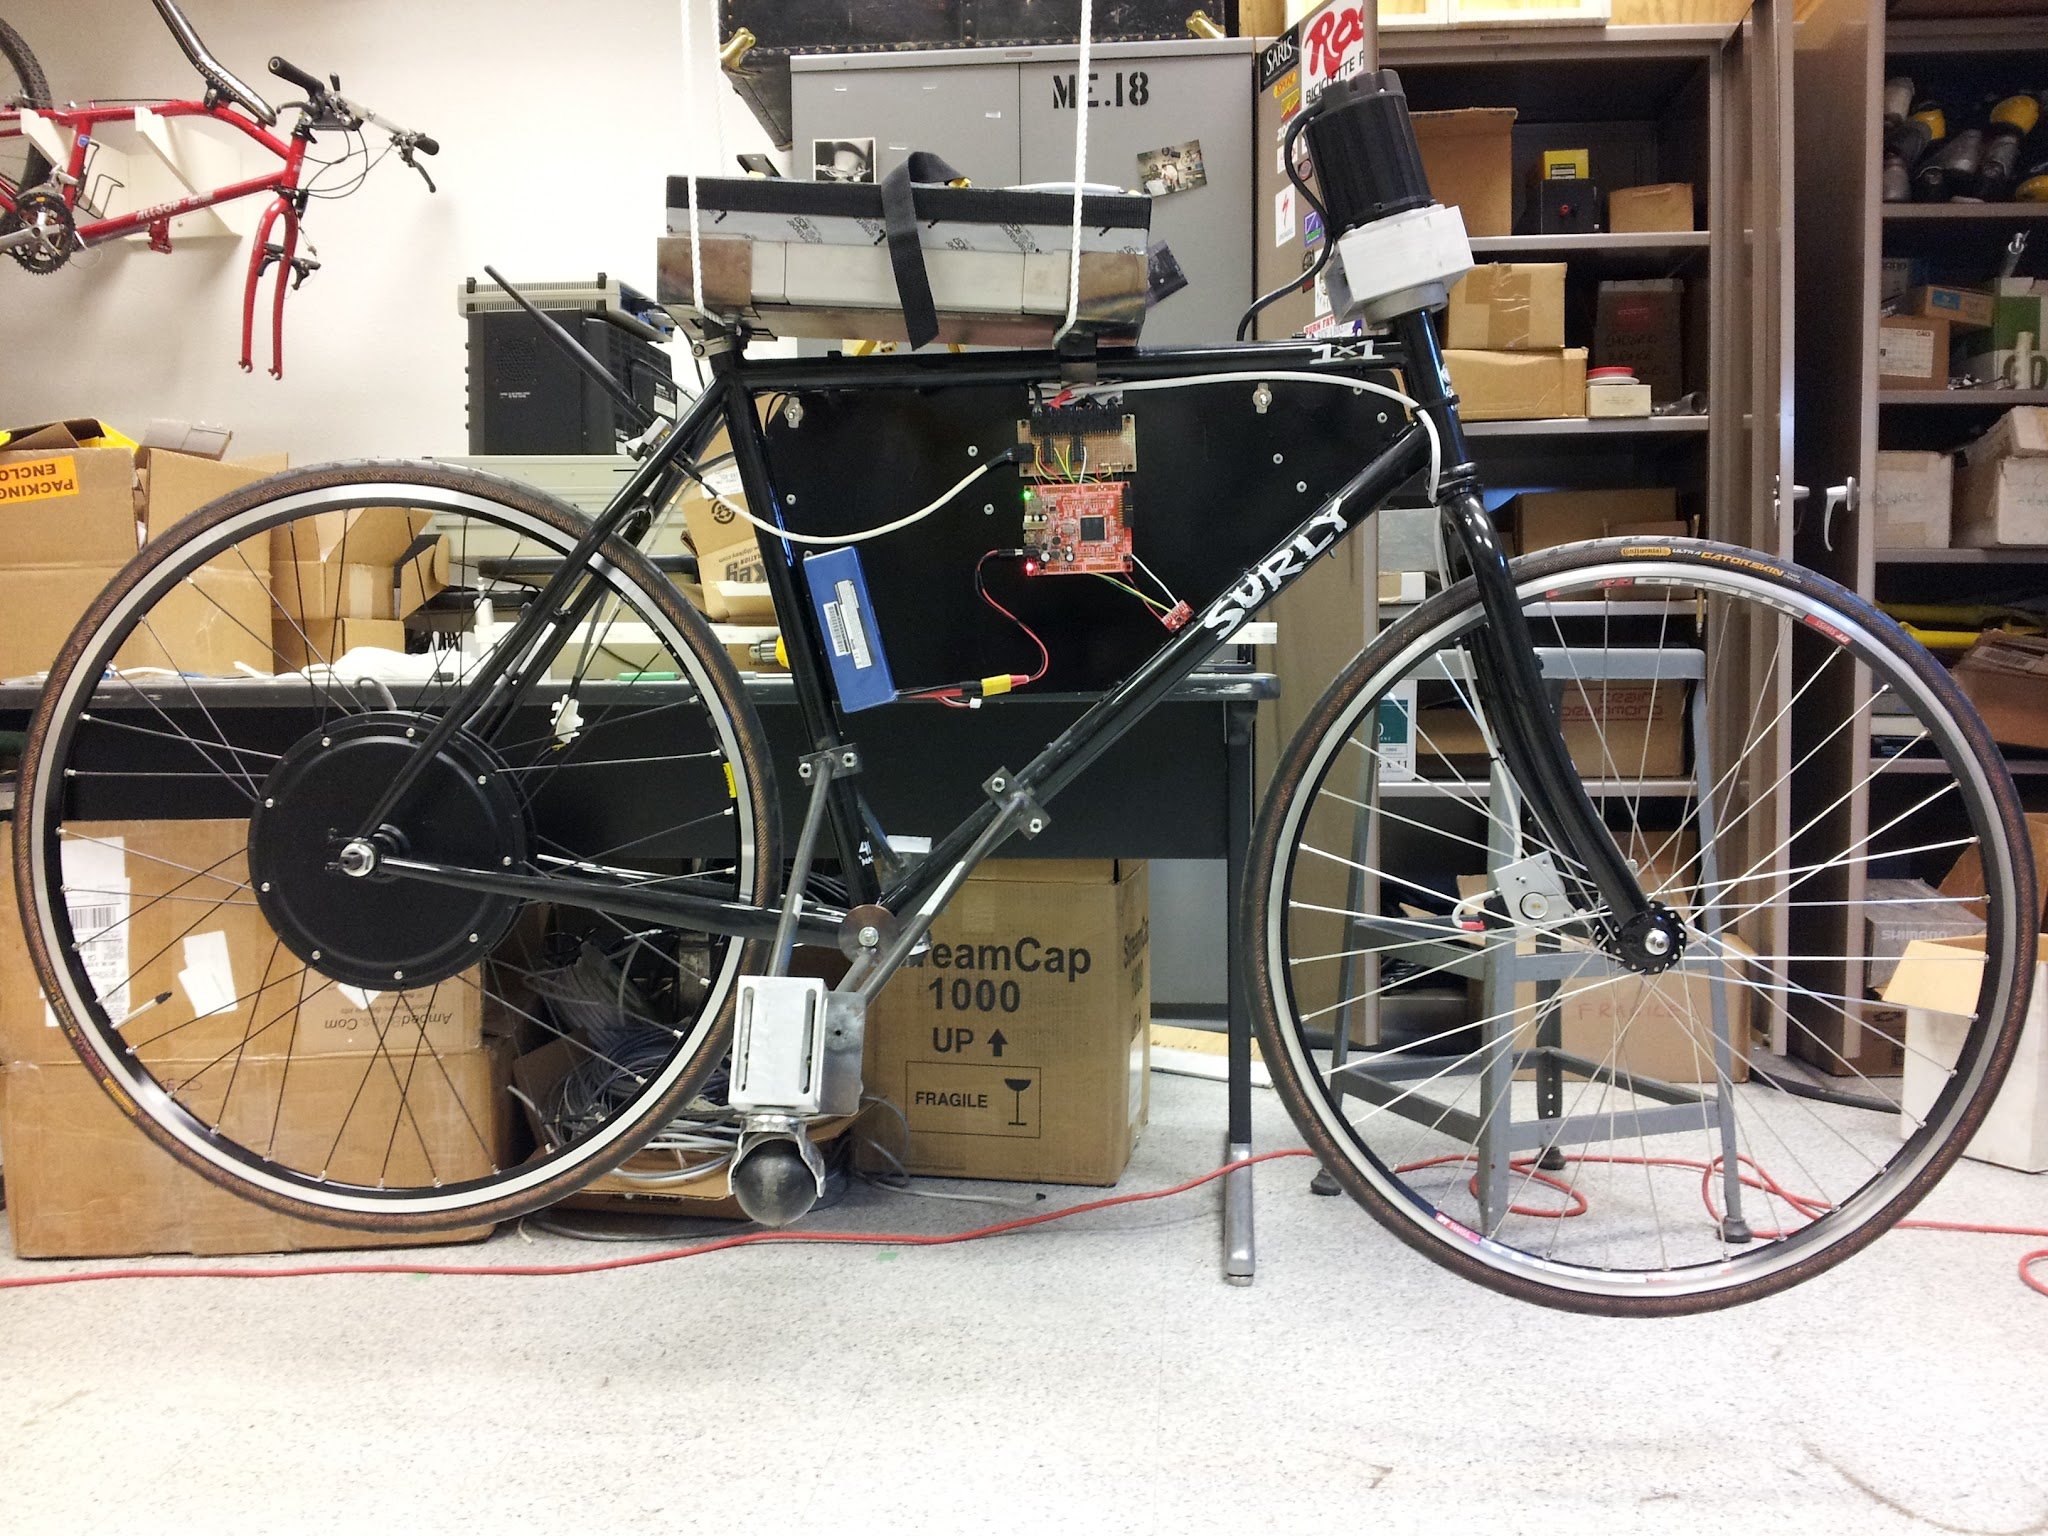
\includegraphics[width=\textwidth]{images/IMG_20120928_153020.jpg}
  \caption{Robot bicycle viewed from the right side.}
  \label{rb:img:rightside}
\end{figure}
\begin{figure}[h]
  \centering
  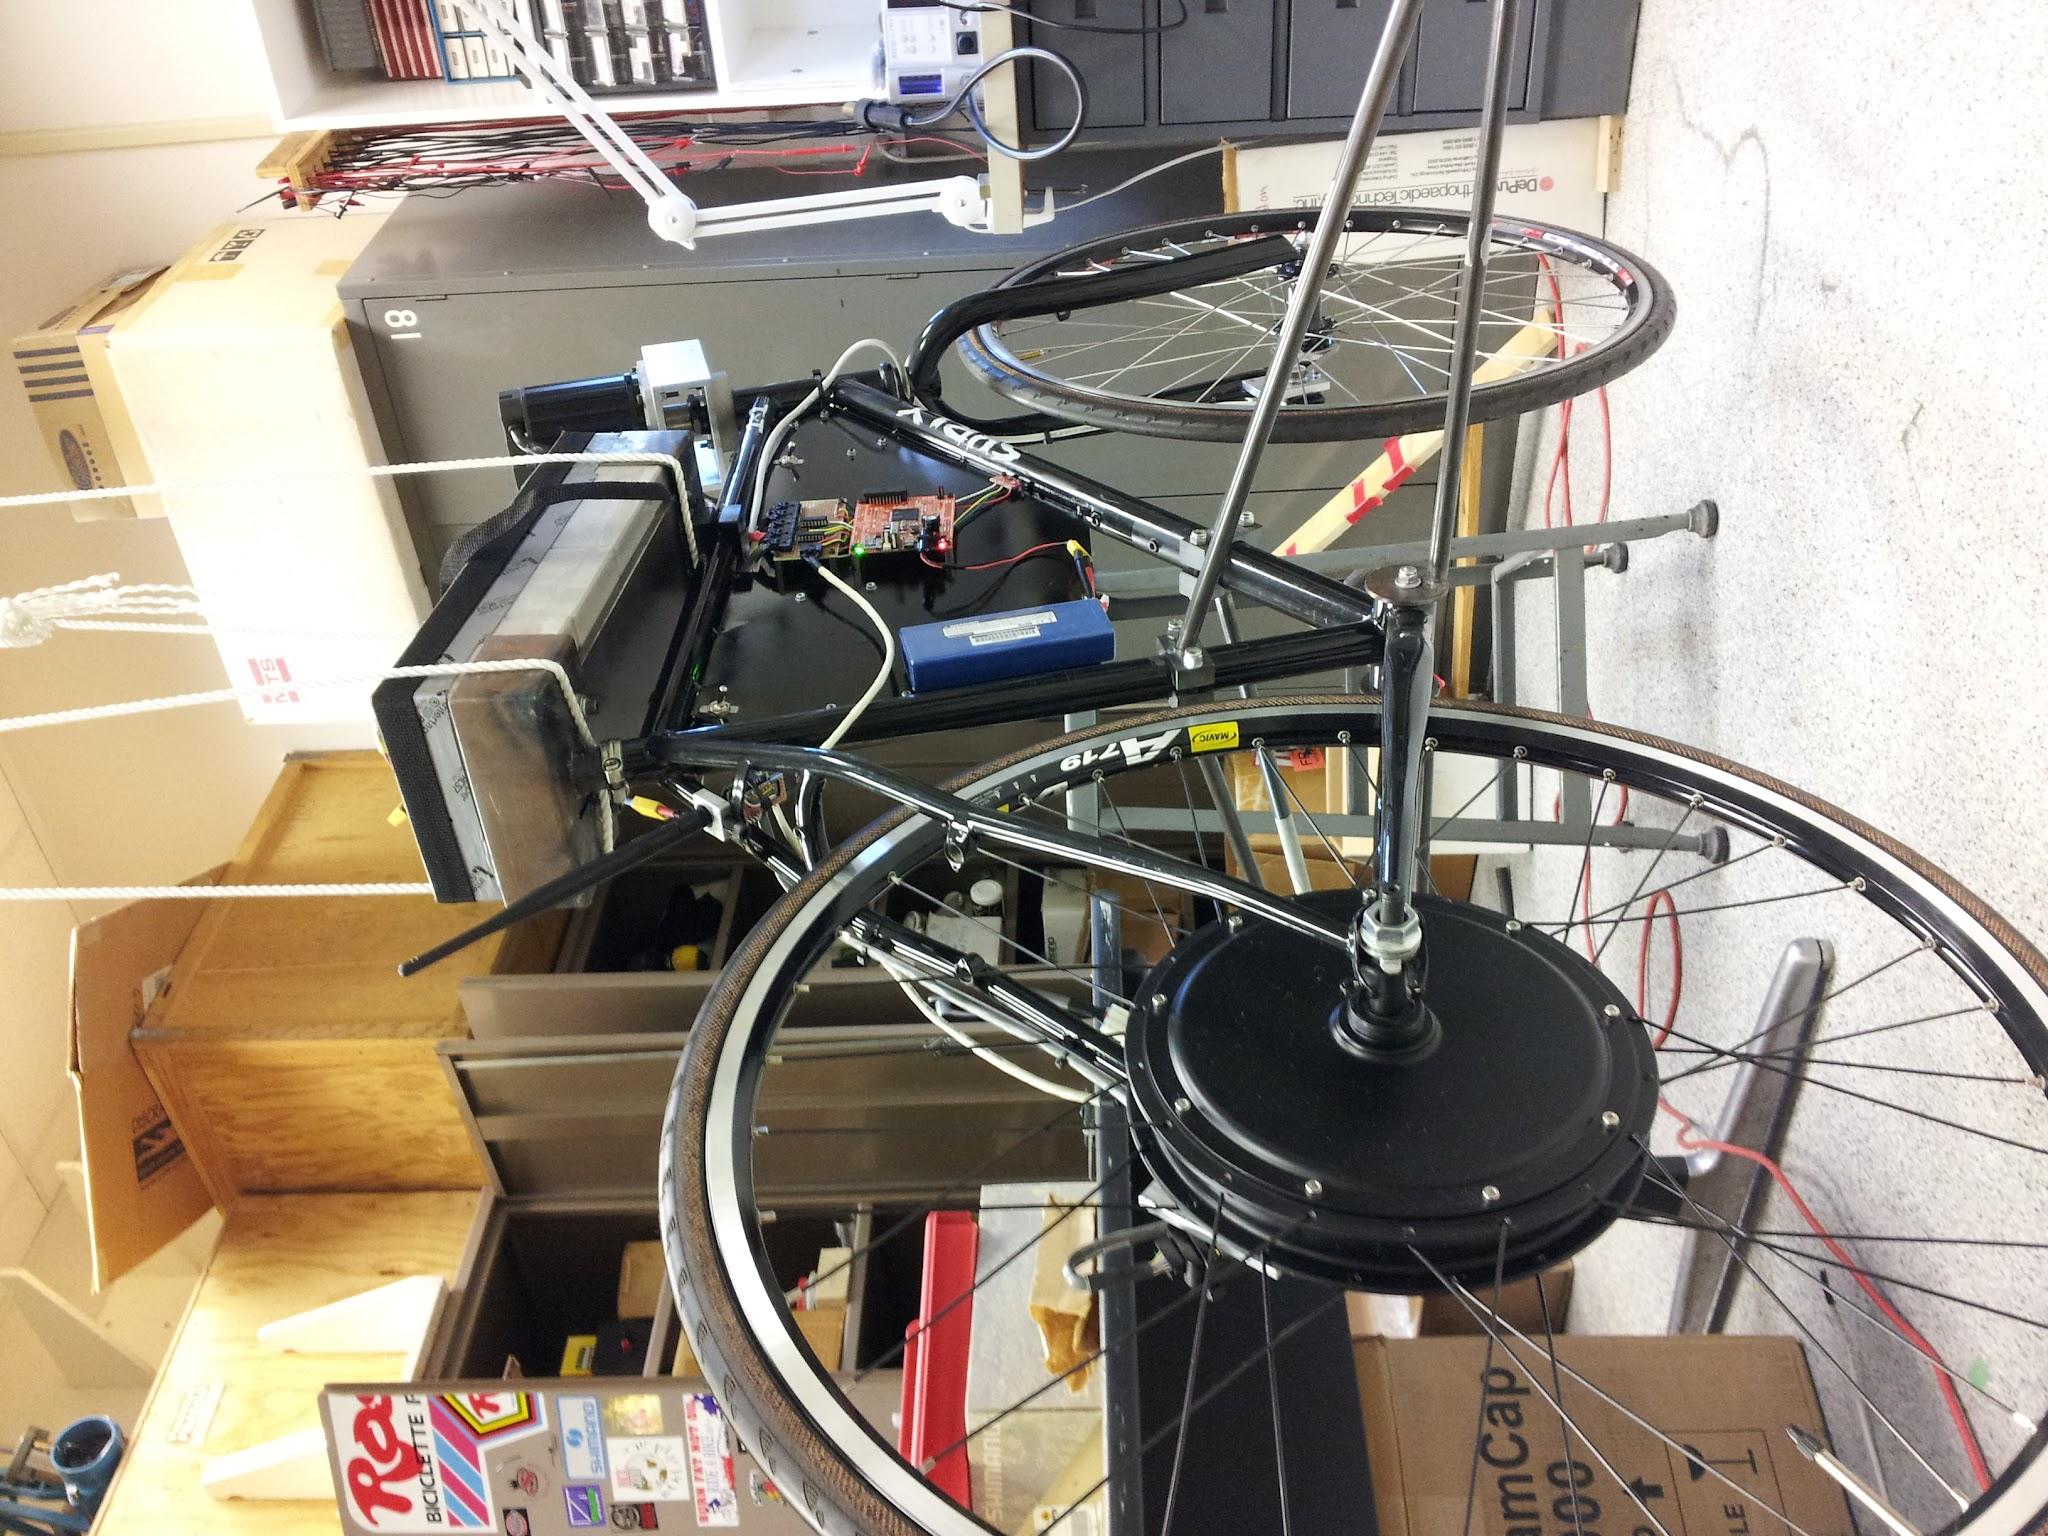
\includegraphics[width=\textwidth,angle=-90]{images/IMG_20120928_153146.jpg}
  \caption{Robot bicycle viewed from the rear right side. The wireless antenna
  is visible behind the batteries, and the attachment of the training wheel
struts to the bicycle frame can also be seen.}
  \label{rb:img:rearrightside}
\end{figure}
\begin{figure}[h]
  \centering
  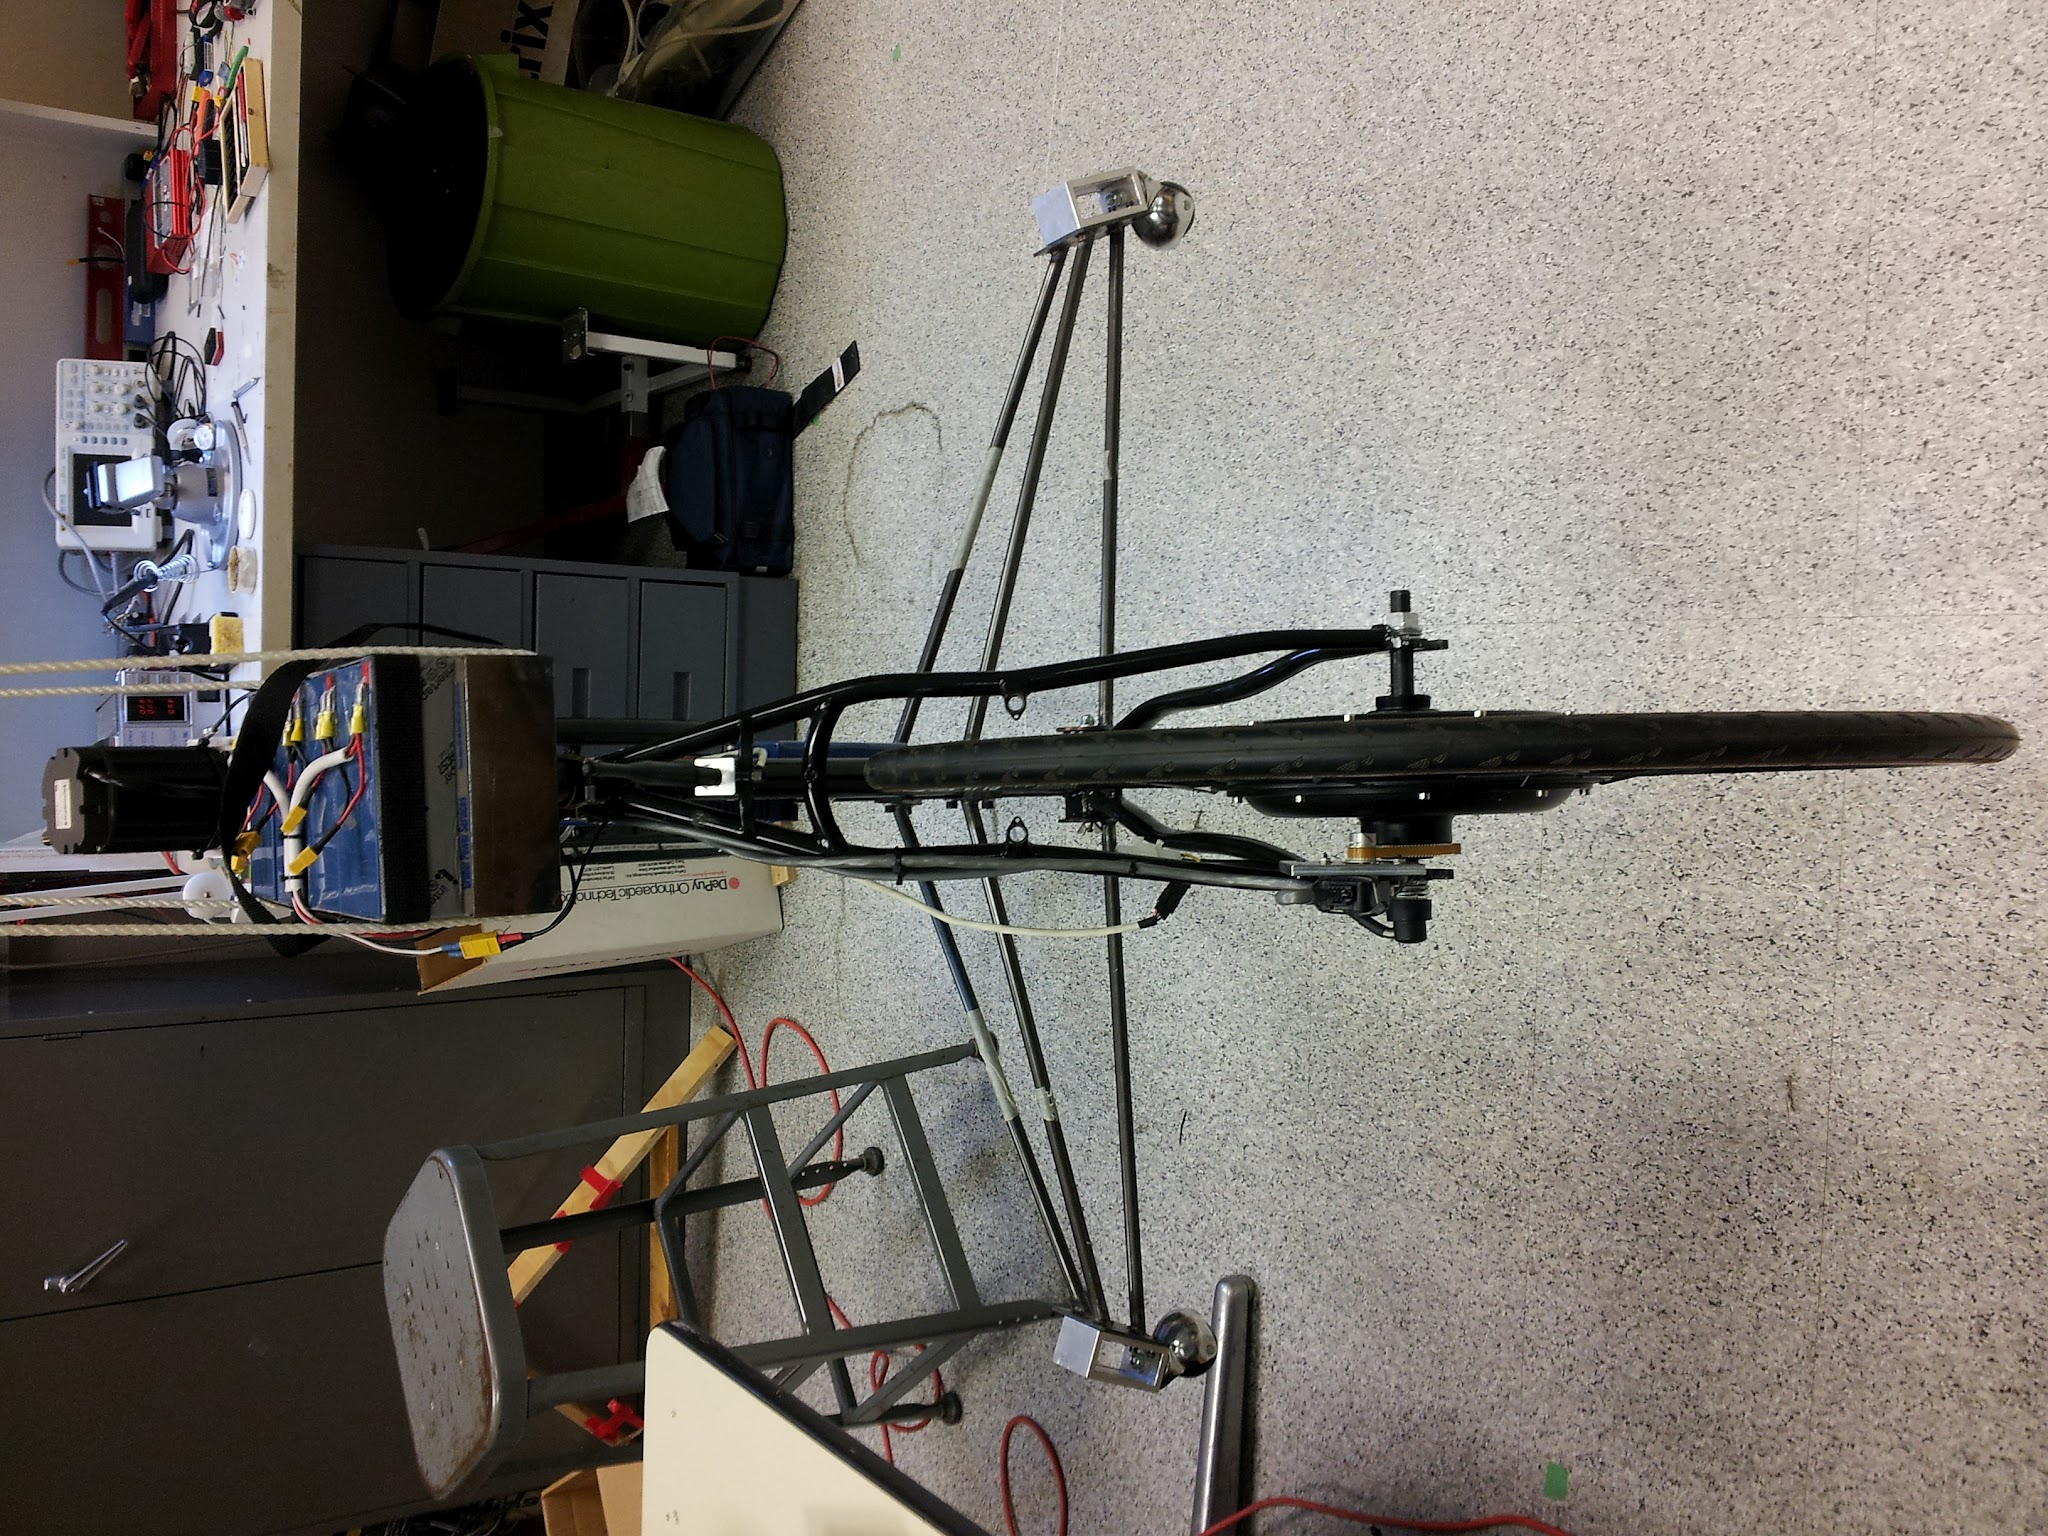
\includegraphics[width=\textwidth,angle=-90]{images/IMG_20120928_153405.jpg}
  \caption{Robot bicycle viewed from the rear.}
  \label{rb:img:rear}
\end{figure}
\begin{figure}[h]
  \centering
  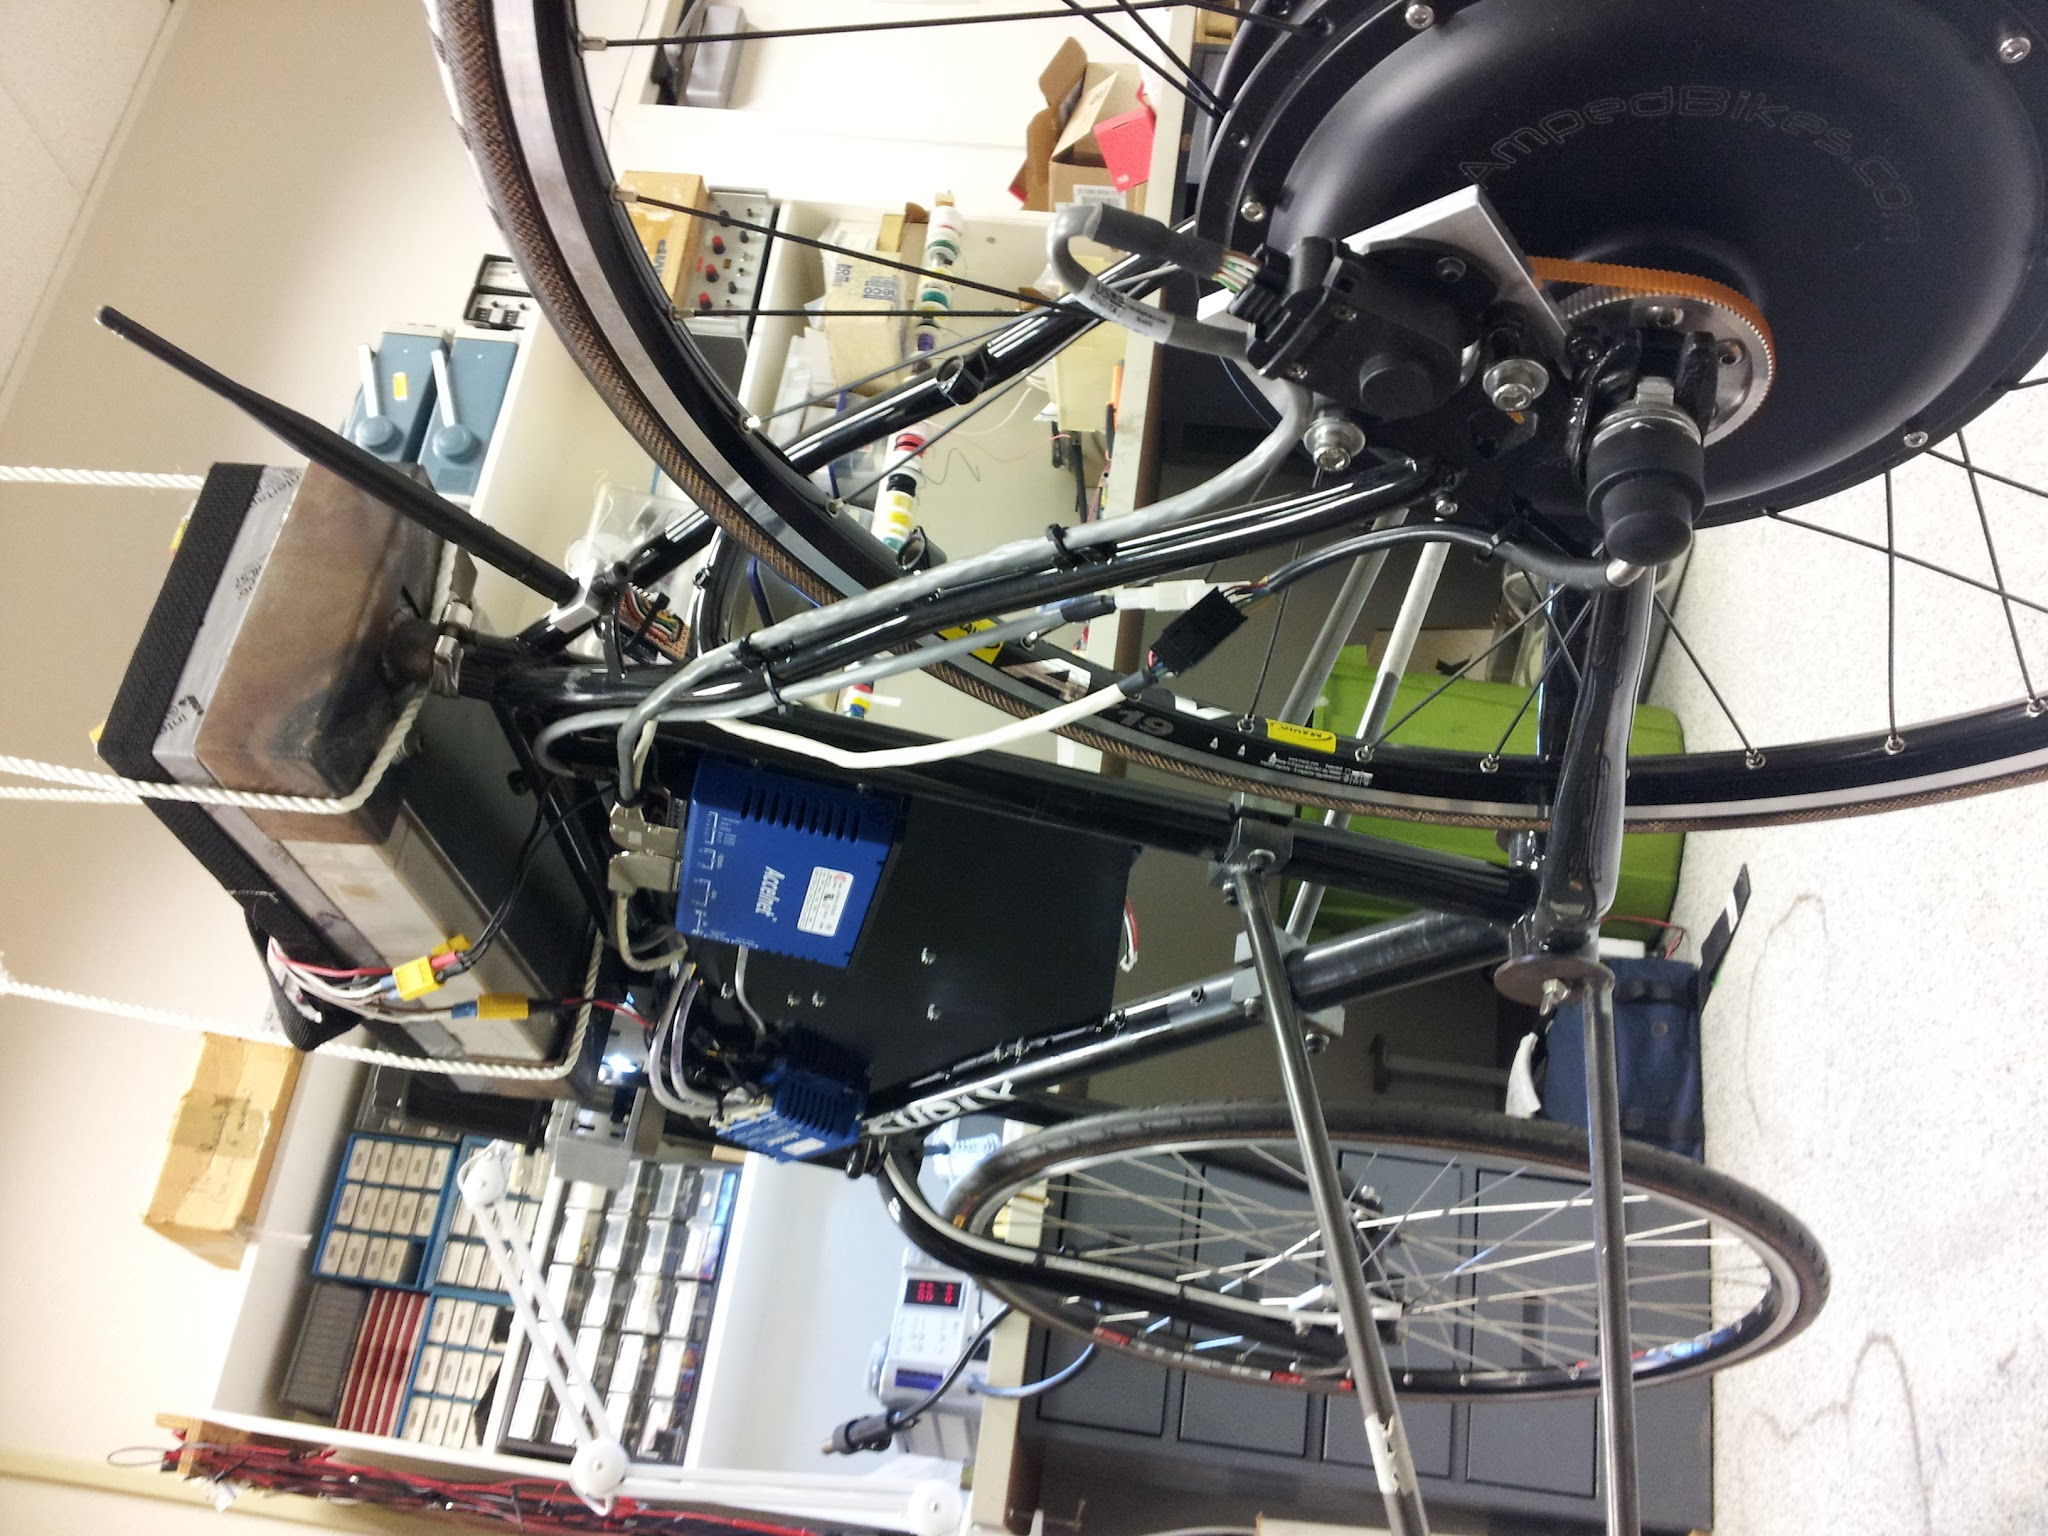
\includegraphics[width=\textwidth,angle=-90]{images/IMG_20120928_153321.jpg}
  \caption{Robot bicycle viewed from the rear left. The motor wiring exits the
    left side of the rear wheel axle. The rear wheel optical encoder is mounted
    to the rear disc brake tabs and is driven by the rear wheel with a
    toothed kevlar belt combined with 100 tooth and 25 tooth pulleys.}
  \label{rb:img:rearleftside}
\end{figure}
\begin{figure}[h]
  \centering
  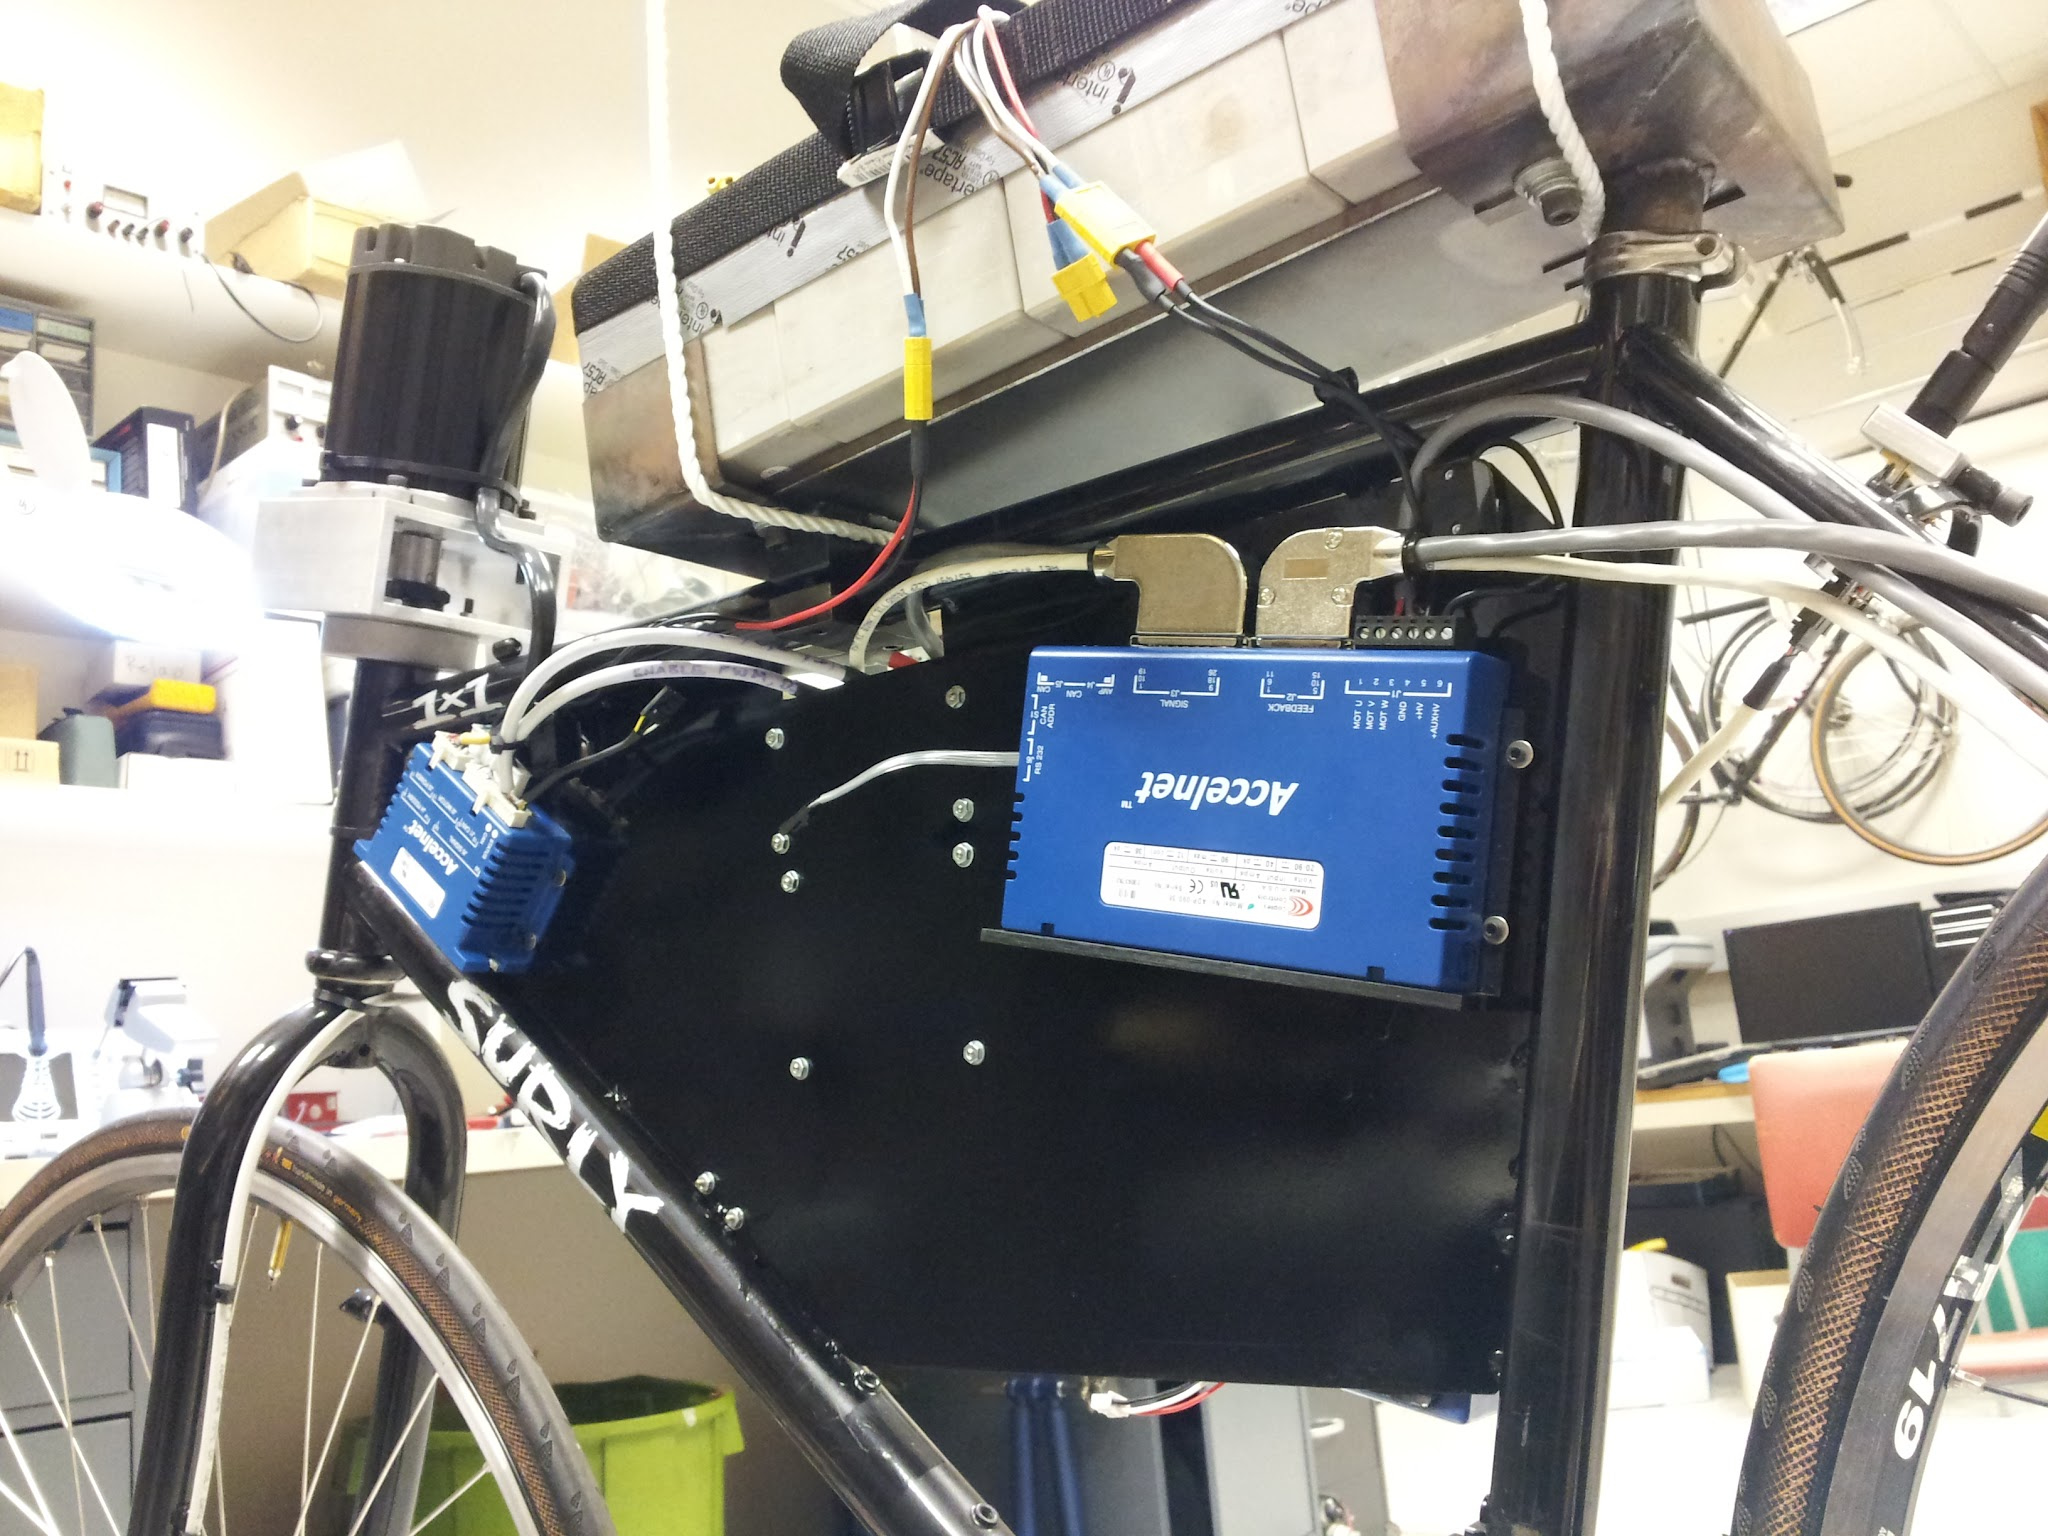
\includegraphics[width=\textwidth]{images/IMG_20120928_153336.jpg}
  \caption{Close up of battery plate, fork motor mount, and digital motor
  drives. The cylindrical plug interfacing the fork motor spindle and the fork
steer tube is visible inside the aluminum box section directly beneath the
steer motor.}
  \label{rb:img:leftsidecloseup}
\end{figure}

A Surly 4130 cromoly steel bicycle frame and fork were used~\cite{Surly2009}.
The frame and fork permit the use of 26'' or 700c wheels, cantilever or disc
brakes, and were chosen because its rugged steel construction permitted
modification without fear of compromising its structural integrity. The frame
was modified by welding an 18 gauge mild steel sheet to the inside of the front
triangle to provide a surface on which to mount the digital motor drives,
microcontroller development board and batteries.

To prevent damage to the robot bicycle in the case of a fall, custom training
wheels were designed and built. The training wheels were composed of casters
positioned approximately 18'' from the frame plane and roughly even with the
bottom bracket. The height of the casters permitted the bicycle to lean
approximately 20$^{\circ}$ before they touched the ground. Each caster wheel
was bolted to a 2'' long 2''x4'' aluminum box section which was in turn bolted
to one side of a small vertical steel plate. On the other side of the steel
plate, three 1/2''x0.0625'' 4130 cromoly steel round tubes were welded -- each
tube connected the steel plate (and hence the casters) to the bicycle frame and
provided sufficient strength and rigidity to handle the loads transmitted
during a fall. Welded to the inboard ends of the three 1/2'' tubes were
brackets which interfaced with the seat tube, down tube, and bottom bracket. The
brackets on either side of the frame were bolted together, thereby sandwiching
the bicycle frame.

Other custom-fabricated mechanical components were the wheel optical encoder
mounts, fork motor mounting hardware, and battery support plate. The details of
each of these components are discussed in \ref{rb:subsec:sensors},
\ref{rb:subsec:actuators}, and \ref{rb:subsec:batteries}, respectively.

\subsection{Physical parameter measurement} \label{rb:subsec:parameters}
The twenty three physical parameters (described in \autoref{chapter2}) of the
robot bicycle were estimated by measuring first the benchmark parameter set,
and then converting those parameters to the gyrostat parameter set using the
equations presented in \autoref{model:parameter_conversion}. It was assumed
that the wheel minor radius was zero (i.e., that the wheels were knife edged).
The resulting parameters are presented in \autoref{rb:tab:parameters}.

\begin{table}[ht]
  \centering
  %\begin{tabular}{rS[table-parse-only]S[table-parse-only]s}
  \begin{tabular}{rccl}
    \toprule
    & {Rear assembly} & {Front assembly} & {Units} \\
    \midrule
    $I_{xx}$ &  1.542 &   0.183 & \si{kg.m^2} \\
    $I_{yy}$ &  3.557 &   0.226 & \si{kg.m^2} \\
    $I_{zz}$ &  3.014 &   0.069 & \si{kg.m^2} \\
    $I_{xz}$ &  0.839 &  -0.010 & \si{kg.m^2} \\
         $J$ &  0.114 &   0.092 & \si{kg.m^2} \\
         $m$ & 34.1   &   2.95  & \si{kg}     \\
         $R$ &  0.336 &   0.336 & \si{m}      \\
         $r$ &  0     &   0     & \si{m}\\
         $a$ &  0.514 &  -0.021 & \si{m}\\
         $b$ & -0.219 &  -0.152 & \si{m}\\
         $c$ &  0.963 &  -0.048 & \si{m}\\
         $l_s$ & \multicolumn{2}{c}{0.343} &  \si{m} \\
    \bottomrule
  \end{tabular}
  \caption{Robot bicycle physical parameters.}
  \label{rb:tab:parameters}
\end{table}

\section{Electrical system description} \label{rb:sec:elec}
\subsection{Microcontroller} \label{rb:subsec:mcu} All functionality related to
control, measurement, and user interaction was implemented by programming an
Olimex STM32-H407~\cite{OlimexSTM32H407} development board. A summary of the
board functionality utilized are shown in Table \ref{rb:tab:mcu}.
\begin{table}[h]
  \centering
  \begin{tabular}{|l|l|}
    \hline
        & ST Microelectronics STM32F407ZGT6 @ 168MHz \\
    CPU & 1MiB flash memory, 192KiB ram, 32-bit memory address space \\
        & Thumb-2 instruction set, single precision floating point \\
    \hline
           & 3 x 16-bit timers in quadrature counting mode \\
    Timers & 32-bit count up timer @ 4MHz \\
           & PWM generation @ 2.563KHz; $2^{16} - 1$ distinct duty cycles \\
    \hline
                   & UART peripheral (115,200 baud 8N1) to XBee Pro radio \\
    Communication  & I2C peripheral @ 400KHz to communicate with IMU \\
                   & SDIO peripheral to log data to micro SD flash memory card \\
                   & JTAG peripheral for flashing and debugging programs \\
    \hline
    General Purpose & Input: momentary switch, motor faults, fork encoder index \\
                    & Outputs: motor enable and direction, lean and steer LEDs \\
    \hline
  \end{tabular}
  \caption{Microcontroller development board functionality.}
  \label{rb:tab:mcu}
\end{table}
The C++11~\cite{C++11} programming language was used to implement all
functionality executed on the development board CPU. Certain language features
such as dynamic memory allocation, runtime type information, and exceptions
were not used due to associated overhead (generated code size or runtime
efficiency). The compiler used was Version 4.7 (update 2) of the GCC ARM
Embedded~\cite{gccARMEmbedded} toolchain was used to compile and link source
code to machine executable code. This ARM maintained version of GCC is
customized to generate efficient machine instructions for ARM embedded
processors.

The real time operating system ChibiOS/RT~\cite{ChibiOS} provided functionality
for threaded execution (concurrency), thread synchronization primitives (mutual
exclusions and semaphores), a filesystem for data logging, an extensible
interactive serial shell, and a high level interface to the development board
hardware peripherals (UART, I2C, SDIO, and GPIOs). ChibiOS/RT directly supports
a large number of development boards, including the Olimex STM32-H407, which
made building and running test code convenient and relatively painless.
Additionally, the very active user community and excellent documentation of
ChibiOS/RT made it easy to troubleshoot problems, ask questions, and get help
while developing the firmware.

The development board was attached to the right side of the sheet in the front
triangle of the frame. Slightly above the development board on the electrical
sheet was a small electrical prototype board which held several small
integrated circuits, Molex connector housings, and two LEDs. The prototype
board connections were soldered directly to the development board so they
effectively acted as a single unit. The Molex connector housings connected
several units to the microcontroller: 1) the optical encoders from both wheels
and fork, 2) the XBee wireless radio, and 3) the enable, fault, direction, and
signal ground pins from the digital motor drives. Wired directly to the
microcontroller development board was a small 7.2V battery
(\autoref{rb:subsec:batteries}) and the inertial measurement unit
(\autoref{rb:subsec:sensors}).


\subsection{Sensors} \label{rb:subsec:sensors}
The robot bicycle was equipped with three optical encoders which measured the
wheel angles and the steer angle. All three optical encoders were
differentially signalled for noise robustness. The front wheel encoder mounted
to the fork but was left disconnected during all experiments due to risk of
damage when the front fork spun more than 180 degrees from straight ahead
(which happened several times in the testing phase of the robot bicycle
design). The steer angle encoder was integrated into the steer
motor~\cite{TeknicM3441} with the optical disc fixed to the motor shaft and
provided 20000 quadrature counts per revolution ($\pi$e-4 rad / quadrature
count) as well as an index signal once per revolution. The wheel optical
encoders~\cite{USDigitalH5} provided an effective 800 quadrature counts per
revolution ($4\pi$e-2 rad / quadrature count) without an index channel. The
wheel encoders were mounted with a custom aluminum adapter to the frame and
fork disc brake mounting tabs. The rear wheel optical encoder is visible in
\autoref{rb:img:rearleftside}; the front wheel optical encoder was mounted
similarly. Since the wheels were symmetric about their axis of rotation, no
calibration was needed for wheel encoders.

The steer encoder was calibrated whenever the cylindrical plug interfacing the
fork motor spindle to the fork steer tube was moved (this was only moved twice,
so only two calibrations were done; the cylindrical plug is visible in
\autoref{rb:img:leftsidecloseup}). A square T fixture was built to hold the
front wheel axle parallel with the rear wheel axle; this was defined to be the
zero steer configuration. The fixture can be seen in
\autoref{rb:img:calibration}. The steer angle calibration involved the
following steps:
\begin{itemize}
  \item Suspend the bicycle from the ceiling and remove both wheels.
  \item Rigidly mount the steer calibration fixture into the wheel dropouts
    (this puts the fork in the zero steer configuration)
  \item Turn on the microcontroller on and call the \verb|calibrate| function.
    This function zeros the steer encoder count and waits for the steer encoder
    index.
  \item Remove the fixture from the front dropouts, and rotate the fork left to
    right 16 times.
  \item Record the steer offset presented by the \verb|calibrate| function.
\end{itemize}
On microcontroller power up or reset, the steer encoder count is set to zero
regardless of the position of the fork. By permanently recording the number of
counts the steer index is from from the zero steer configuration, this offset
can be set during a fork homing procedure when the steer index is triggered.
This functionality was implemented in the \verb|homefork| function and was run
every time the microcontroller was reset or powered up.

\begin{figure}[ht]
  \centering
  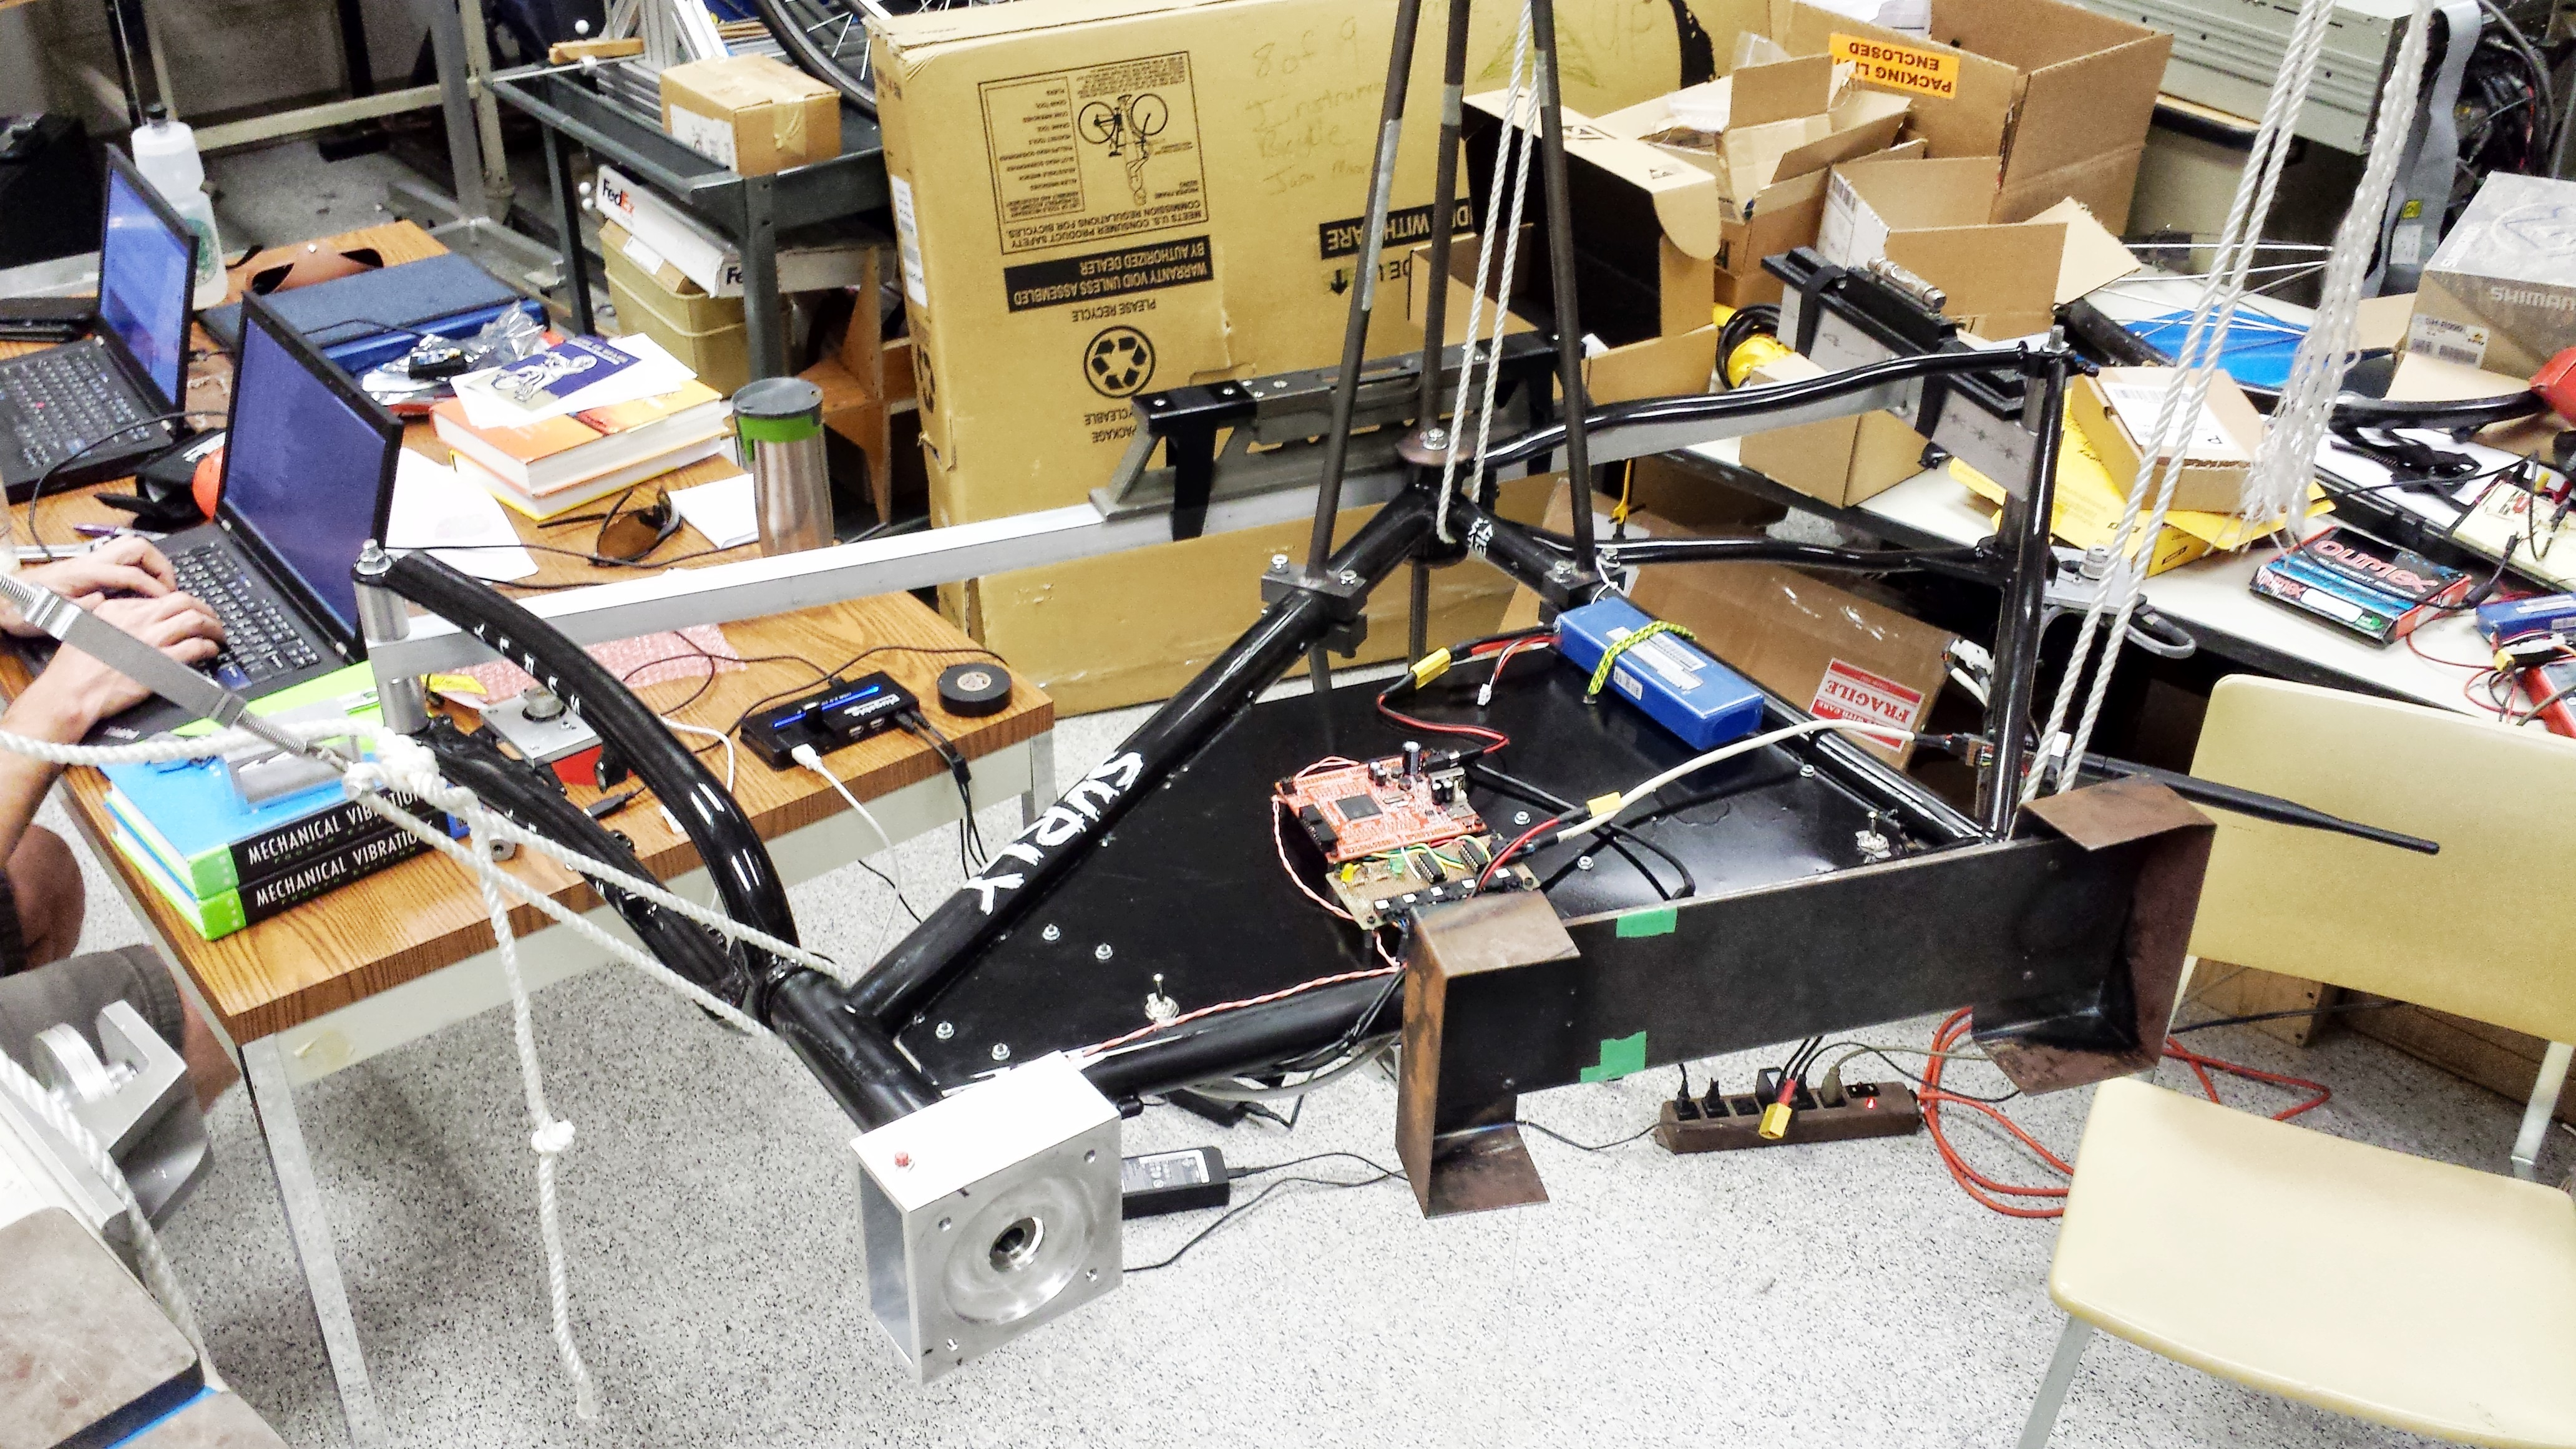
\includegraphics[width=\textwidth]{images/20130711_163732_2.jpg}
  \caption{Calibration of steer angle encoder, accelerometer, and rate
    gyroscope ($\phi=-\pi/2$ configuration). The steer calibration fixture
    ensured $\delta=0$ and provided surfaces to rest the bubble levels (visible
    on far side of bicycle frame). Two turnbuckles were used to make minor
  orientation adjustments to level the frame (visible on left side of image).}
  \label{rb:img:calibration}
\end{figure}

A combined rate gyroscope and accelerometer MEMS
sensor~\cite{InvensenseMPU6050} was fixed to the underside of the battery pack
plate as shown in \autoref{rb:img:imuplacement}. The gyroscope and
accelerometer sensor axes were assumed to be aligned with each other since they
are manufactured on the same piece of silicon. The sensor $\bm{s}_x-\bm{s}_y$
plane was approximately parallel to the plane of the battery plate, with
$\bm{s}_y$ pointed approximately forward, $\bm{s}_y$ to the left, and
$\bm{s}_z$ down.

As described in Chapter 1, the bicycle model introduces set of dextral unit
vectors fixed to the rear frame $R$ of the bicycle, with $\bm{r}_z$ parallel to
the steer axis and down, $\bm{r}_y$ perpendicular to the frame plane and to the
right, and $\bm{r}_x = \bm{r}_y \times \bm{r}_z$ ($\bm{r}_x$ points forward and
slightly up when the bicycle is in the reference configuration). Fixed to the sensor $S$
are a set of dextral unit vectors with $\bm{s}_x$ and $\bm{s}_y$ in the plane
of the integrated circuit, and $\bm{s}_z$ normal to the plane of the integrated
circuit. To orient the sensor relative to the bicycle, first align $S$ with
$R$, then apply the following successive body-fixed ZXY rotations: $\alpha -
\pi/2$, $\beta$, $\gamma$. The first rotation was offset by $-\pi/2$ so that
all three angles were near zero.

\begin{figure}[ht]
  \centering
  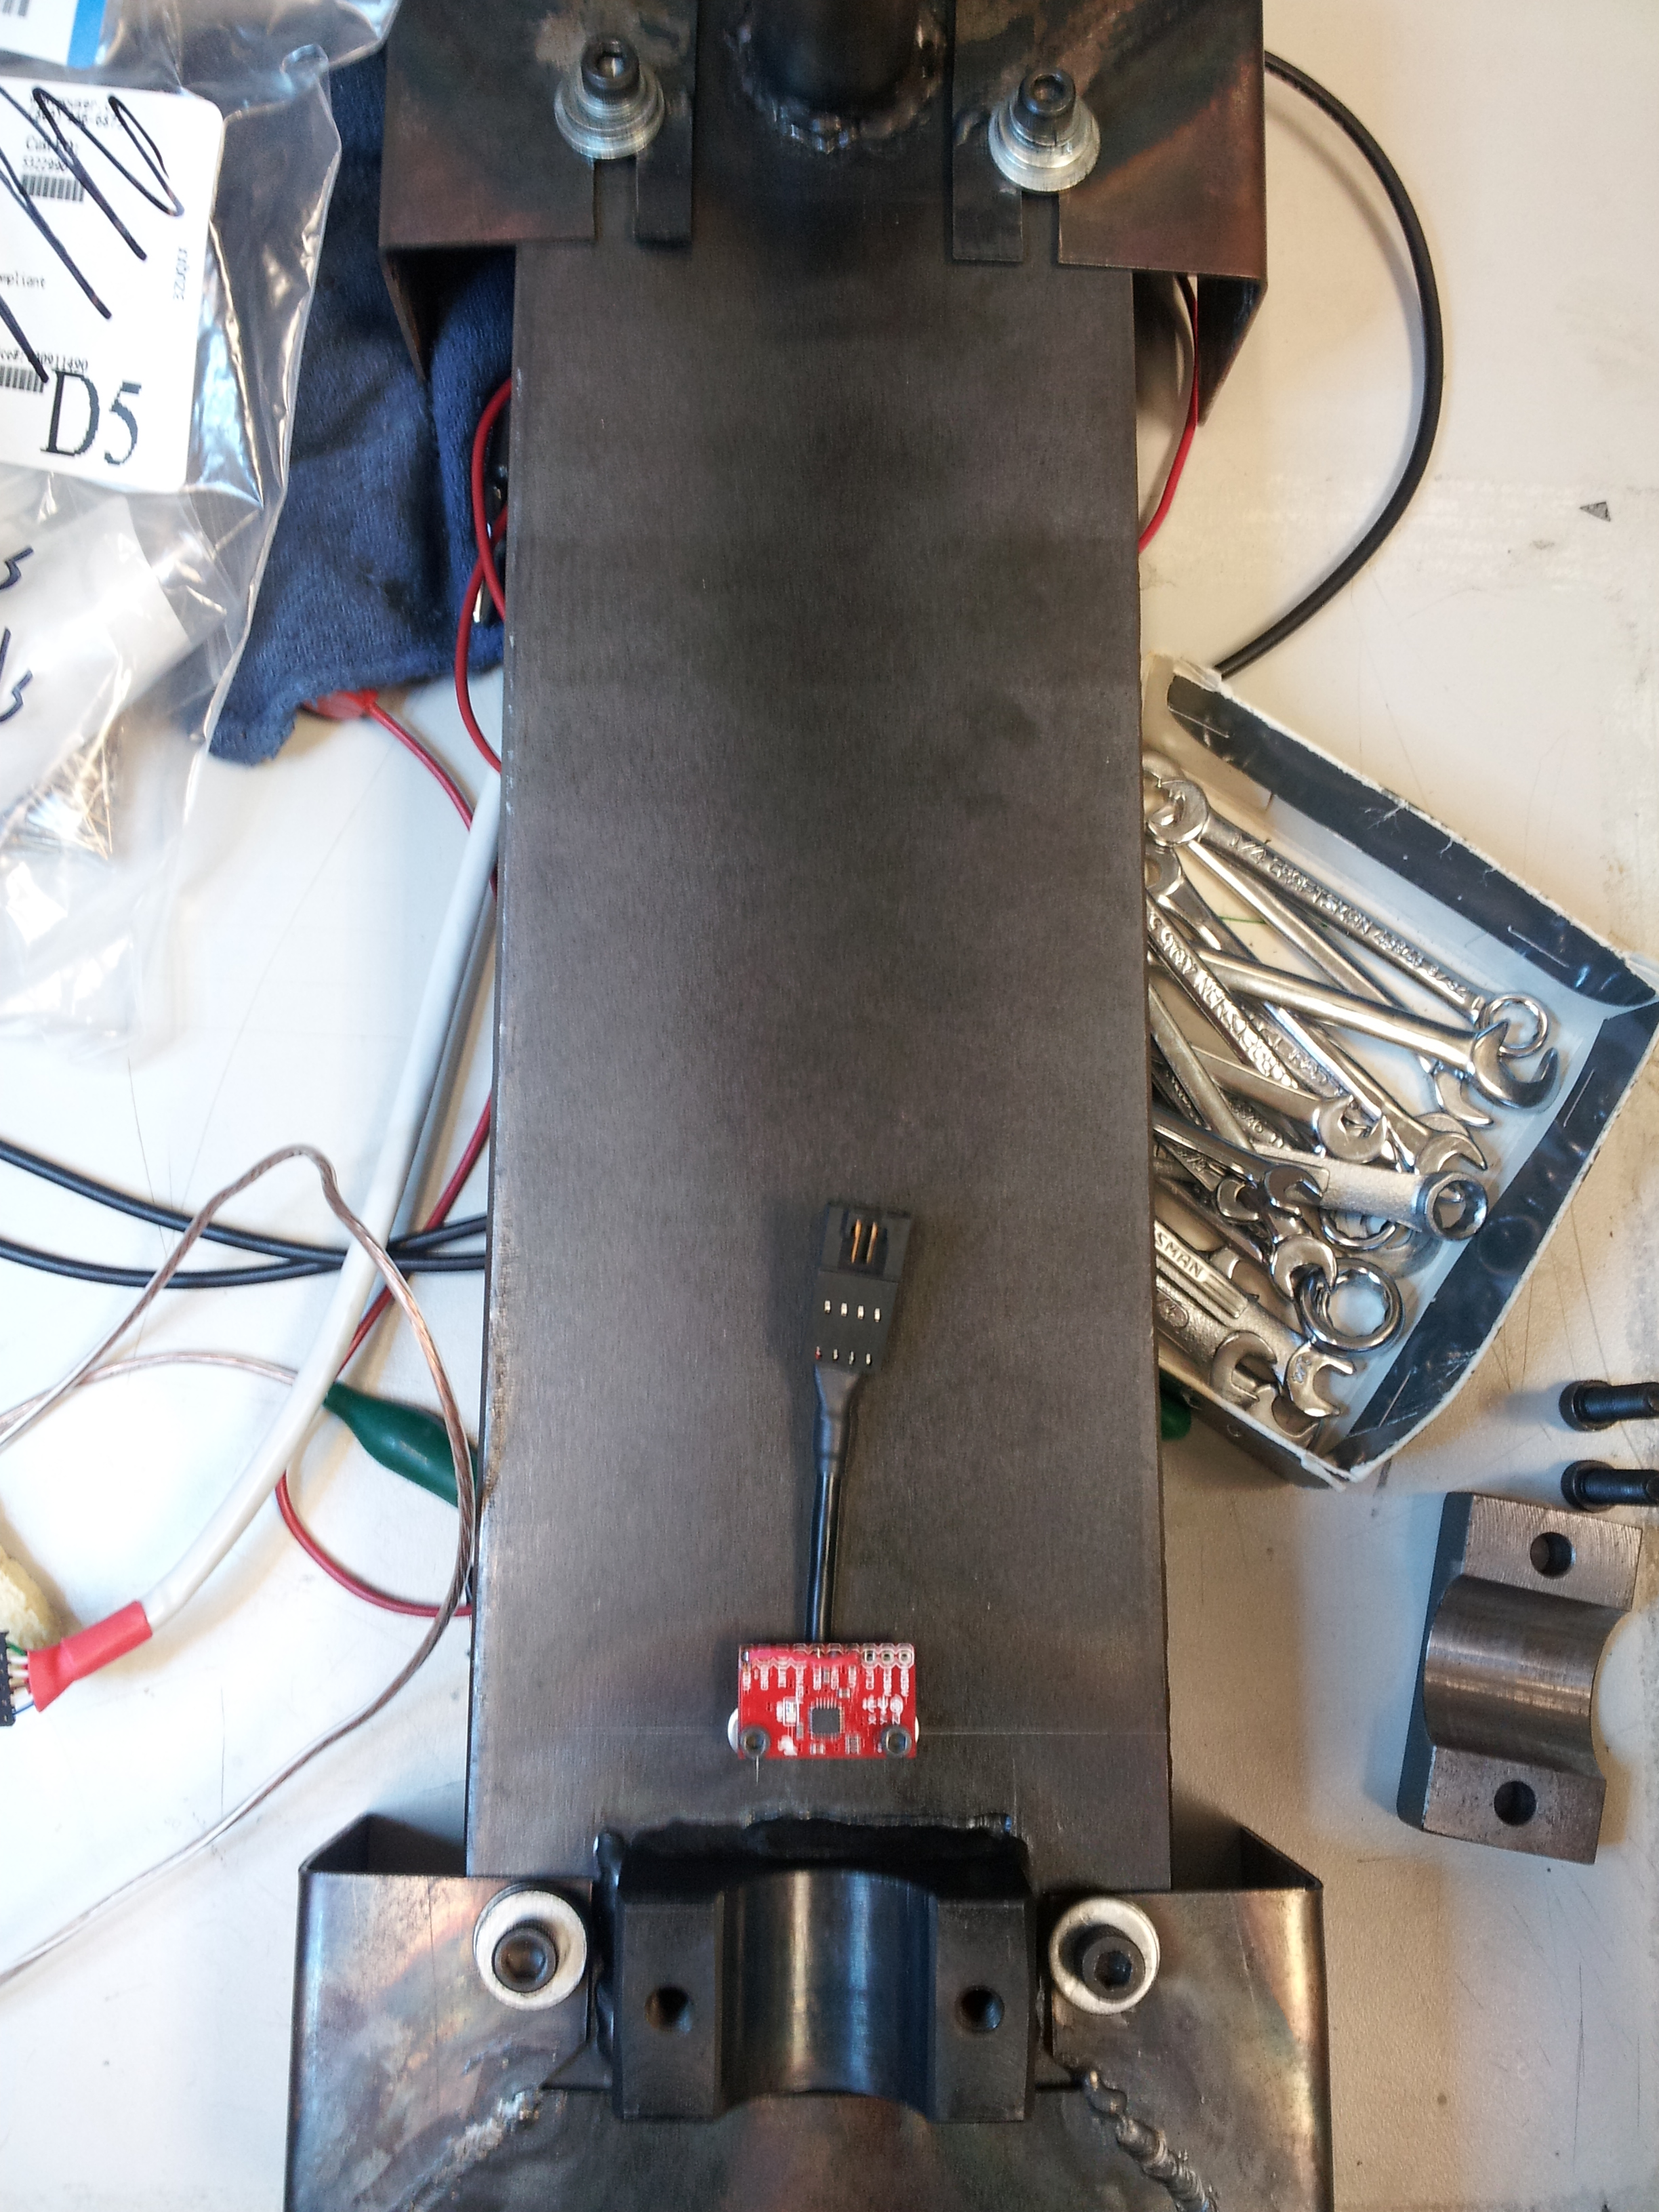
\includegraphics[width=.6\textwidth,angle=90]{images/IMG_20130325_195226.jpg}
  \caption{Rate gyroscope and accelerometer sensor placement on bottom of
  battery support plate. The top tube clamshell bracket is visible on the right side of
the image (forward end of battery plate). On the left side of the image the
seat post is partially visible. The mounting hardware for the battery box is also
visible.}
  \label{rb:img:imuplacement}
\end{figure}

To determine the three angles $\alpha$, $\beta$, and $\gamma$, the static
acceleration was measured in three sensor directions ($\bm{s}_x$, $\bm{s}_y$,
$\bm{s}_z$) in six unique configurations. The six configurations are those that
would be obtained if $R$ were aligned with and fixed to the edges of a perfect
cube and the cube was laid on a level surface on each of its six sides.  These
six configurations correspond to the following bicycle orientations:
$\phi=\pm\pi/2$ (frame plane horizontal), $\phi=0$ and $\theta_R = \{-\pi/2, 0,
\pi/2, \pi\}$ (frame plane vertical, two horizontal steer axis orientations and
two vertical steer axis orientations). The sensed acceleration in the three sensor
directions was recorded for approximately sixty seconds while the bicycle was
in each each of the six configurations.

When at rest, the accelerometer senses the gravitational field as if it were
accelerating \textit{upwards} at $g$, this corresponds to $-g\bm{n}_z$.
Resolving $-g\bm{n}_z$ into the three sensor measurement directions yields
\begin{align}
  \label{rb:eq:imux}
-g\bm{n}_z \cdot \bm{s}_x &= g \left(- s_{\alpha}
s_{\beta} s_{\gamma}
s_{\phi} + s_{\alpha}
s_{\theta} c_{\gamma}
c_{\phi} + s_{\beta}
s_{\gamma} s_{\theta}
c_{\alpha} c_{\phi} +
s_{\gamma} c_{\beta}
c_{\phi} c_{\theta} +
s_{\phi} c_{\alpha}
c_{\gamma}\right) \\
%
  \label{rb:eq:imuy}
-g\bm{n}_z \cdot \bm{s}_y &= g \left(- s_{\alpha}
s_{\phi} c_{\beta} -
s_{\beta} c_{\phi}
c_{\theta} + s_{\theta}
c_{\alpha} c_{\beta}
c_{\phi}\right) \\
%
  \label{rb:eq:imuz}
-g\bm{n}_z \cdot \bm{s}_z &= g \left(s_{\alpha}
s_{\beta} s_{\phi}
c_{\gamma} + s_{\alpha}
s_{\gamma} s_{\theta}
c_{\phi} - s_{\beta}
s_{\theta} c_{\alpha}
c_{\gamma} c_{\phi} +
s_{\gamma} s_{\phi}
c_{\alpha} - c_{\beta}
c_{\gamma} c_{\phi}
c_{\theta}\right)
\end{align}
The goal of the calibration was to convert the measured acceleration to the
true acceleration, and for this reason the following slightly non traditional
(yet equally representative) form of the acceleration sensor model was used
\begin{align}
  \label{rb:eq:sensormodel}
  \left[
    \begin{matrix}
      -g\bm{n}_z \cdot \bm{s}_x \\
      -g\bm{n}_z \cdot \bm{s}_y \\
      -g\bm{n}_z \cdot \bm{s}_z
    \end{matrix}
  \right]
  &=
  \left[
    \begin{matrix}
      S_{xx} & S_{xy} & S_{xz}\\
      S_{xy} & S_{yy} & S_{yz}\\
      S_{xz} & S_{yz} & S_{zz}
    \end{matrix}
  \right]
  \left[
    \begin{matrix}
      a_{x} \\
      a_{y} \\
      a_{z}
    \end{matrix}
  \right]
  +
  \left[
    \begin{matrix}
      b_{x} \\
      b_{y} \\
      b_{z}
    \end{matrix}
  \right]
\end{align}
where $a_x, a_y, a_z$ are the raw sensor measurements (in units of bits), $b_x,
b_y, b_z$ are biases (in units of m/s$^2$), $S_{xx}, S_{yy}, S_{zz}$ are the
sensitivities, and $S_{xy}, S_{yz}, S_{xz}$ are the cross axis sensitivities,
both of which have units of m/s$^2$/bit. Cross axis sensor symmetry was
assumed, i.e., $S_{xy} = S_{yx}$.

Equating the right side of Equations \ref{rb:eq:imux}-\ref{rb:eq:imuz} with the
right side of \autoref{rb:eq:sensormodel}, evaluating at the value of lean
$\phi$ and pitch $\theta$ corresponding with a particular configuration, and
taking the time series mean of each of the raw measurements $a_x, a_y, a_z$, we
obtain three equations with twelve unknowns. Repeating for each of the six
configurations, we obtain an overdetermined system of eighteen equations in
twelve unknowns. The twelve unknowns are the six sensitivites, the three
biases, and the three orientation angles relating the sensor frame to the
bicycle frame. This overdetermined system of equations was solved by the method
of least squares to obtain the following sensitivities, biases, and orientation
angles
\begin{align}
  \left[
    \begin{matrix}
      S_{xx} \\
      S_{yy} \\
      S_{zz} \\
      S_{xy} \\
      S_{yz} \\
      S_{xz}
    \end{matrix}
  \right]
  &=
  \left[
    \begin{matrix}
      \num{5.9898e-4} \\
      \num{5.9534e-4} \\
      \num{5.8288e-4} \\
      \num{-5.4766e-7} \\
      \num{-1.6455e-6} \\
      \num{1.9272e-6}
    \end{matrix}
  \right] \text{m/s$^2$/bit} \\
  \left[
    \begin{matrix}
      b_{x} \\
      b_{y} \\
      b_{z}
    \end{matrix}
  \right]
  &=
  \left[
    \begin{matrix}
      -0.5700 \\
       0.0514 \\
       1.1690
    \end{matrix}
  \right] \text{\si{m/s^2}} \\
  \left[
    \begin{matrix}
      \alpha \\
      \beta \\
      \gamma
    \end{matrix}
  \right]
  &=
  \left[
    \begin{matrix}
      0.0031 \\
      0.3230 \\
     -0.0182
    \end{matrix}
  \right] \text{rad}
\end{align}
The diagonal entries of $S$ were very close to the manufacturer specified
sensitivity of \num{5.9876e-4} m/s$^2$/bit. The diagonal entries were greater than
the off-diagonal entries by more than two orders of magnitude, indicating the
cross axis sensitivity was less than 1\%, also in line with the manufacturers
specifications. The means of three rate gyroscope measurements axes were
computed for each static configuration, and were found to be independent of
configuration (as expected). These means were used as biases for the
measurement of the bicycle frame angular velocity and were found to be
\begin{align}
  E[\omega_x] &= -0.1204\text{ rad/s}\\
  E[\omega_y] &=  0.0316 \text{ rad/s}\\
  E[\omega_z] &=  0.0100 \text{ rad/s}
\end{align}
Since a rate table or other convenient means of calibrating the gyroscope
sensitivities was not available, the manufacturer published gyroscope
sensitivities were used.

%For each configuration, replacing the term to the left of the equality with the

%mean of each respective sensor axis measurement, and evaluating the terms to

%the right of the equality at the value of lean $\phi$ and pitch $\theta$

%associated with that configuration, Equations \ref{rb:eq:imux}-\ref{rb:eq:imuz}

%yield a system of three equations in three unknowns: $\alpha, \beta, \gamma$.

%This yield a system of 18 equations in three unknowns.





%A calibration procedure to determine the orientation of the
%sensor axes relative to the frame axes (as defined by the model) was performed
%by accurately orienting the bicycle in six orientations: 1, 2) steer axis
%vertical (two configurations); 3, 4) steer axis horizontal, rear axle axis
%vertical (two configurations); 5, 6) steer axis horizontal, rear axle axis
%horizontal (two configurations). Said another way, the six orientations are
%those that would be obtained if the bicycle body fixed coordinates were aligned
%with and fixed to the edges of a perfect cube, and the cube was laid on a level
%surface on each of its six sides while data was collected from an accelerometer
%fixed to the cube but whose axes didn't aligned with the cube edges.
%
%The six orientations were obtained by suspending the bicycle by ropes from three
%points of attachment and using a turnbuckle on two of the ropes to level the
%desired surface in two directions. Two precision horizontal bubble levels were
%attached to the frame 90 degrees apart to permit levelling in both directions.
%Once levelled, the bicycle was left to rest for approximately 5 minutes to
%allow for small swinging and twisting oscillations to die out; this was also
%aided by suspending a weight from the frame with fishing line and hanging it
%into a bucket of water. The bucket of water provided some dissipation which
%helped damp out vibrations. Once stationary (within the limits of the vibrating
%building), data collection was initiated for a period of approximately 60
%seconds.


\subsection{Actuators} \label{rb:subsec:actuators}
The robot bicycle was equipped with a rear wheel hub motor to drive the rear
wheel and a fork motor to steer the bicycle. Both motors were brushless DC
motors and were interfaced to the microcontroller with Copley Controls digital
motor drives (fork: ACJ-055-18~\cite{CopleyACJ}, rear wheel:
ADP-090-36~\cite{CopleyADP}). Both digital motor drives were configured in
current control mode and internally implemented a PI current (with gains
automatically selected via manufacturer software based upon motor parameters)
controller that operated at 30kHz. The current commands were generated by the
microcontroller as 3.3V pulse width modulated (PWM) signals which were
converted by the motor drives to the appropriate high voltage, high current PWM
signals to the motor windings. The bicycle control system was designed to
generate applied joint torques as control signals, which were then scaled by
the respective motor torque constants before generating the current command PWM
signal.

The rear wheel was built with an electric hub motor~\cite{AmpedBikes}. The
manufacturer supplied rim and spokes were of extremely low quality (very weak,
untrue, and noticeably inertially non-symmetric), so they were replaced with DT
Swiss 2.0mm stainless steel spokes and Mavic model A719, 700c diameter, 36 hole
rim. The rear hub axle served as the motor stator and armature with the three
motor power leads exiting the left side of the axle. The motor field magnets
were fixed to the inside of the hub shell and rotated along with the spokes,
rim, and tire when current was applied to the motor windings. This motor
configuration is commonly known as the ``outrunner'' configuration. No
manufacturer specifications were available for this motor, so the motor torque
constant was determined experimentally by applying a constant rear wheel
current $I_R$ with while the wheel was off the ground and measuring the angular
response. The spin inertia $J_r$ of the rear wheel was measured
(\autoref{rb:subsec:parameters}), and the idealized DC motor equation
$J_r\ddot{\theta}_R = K_t I_r$ was integrated twice with respect to time
(constant current assumed and $\theta_R(0)=\dot{\theta}_R(0) = 0$) to obtain
$\theta = \frac{K_t I_r}{2J_r}t^2$. A least squares fit was then used to
estimate $K_t=6.6$ Nm/A. Since a PI speed controller was implemented to control
rear wheel rate, it was not critical to know $K_t$ precisely (PI controllers
perform reasonably well even when system parameters are not well known); for
this reason we didn't expend any effort to more accurately determine $K_t$.

The fork motor~\cite{TeknicM3441} was bolted to an aluminum box section which
in turn was bolted to a custom upper headset. The custom upper headset was
pressed into the upper end of the bicycle steer tube with green Loctite to
ensure it would not twist relative to the frame when motor torques were
applied. In contrast to the rear wheel hub motor, the fork motor stator and
armature windings were fixed to the outer portion of the motor (fixed to the
bicycle frame) and the field magnets were fixed to the motor output shaft.  The
motor output shaft was equipped with a key-way which was mated to a circular
plug fixed to the inside of the steer tube. The circular plug was rigidly
attached to the steer tube in the same way a threaded bicycle stem wedge
expander attaches to the bicycle steer tube. The upper portion of the circular
plug (which mates with the motor shaft) was bored with a hole to match the
diameter of the motor output shaft, and an internal key-way was cut with a
wire-cut electrical discharge machine. Once the motor was secured, a set
screw was threaded into the upper portion of the plug to make contact with the
motor key. This design permitted the fork to be driven directly by the motor
without the use of a gearbox, and still permitted the motor to be removed
easily if necessary. Most importantly, the design had no backlash between the
motor shaft and the fork. A previous design was attempted which made use of a
precision gearbox, but it was found to have unacceptable levels of backlash.
Since the sign of the steer angle rate frequently changes during normal
operation of a bicycle, any backlash between the motor fork is extremely
undesirable.

\subsection{Batteries} \label{rb:subsec:batteries}
Four 12.0V sealed lead acid (SLA) batteries were wired in series and used to
power the motors and the digital motor drives. The SLA batteries were arranged
in a row of four and tightly bound to each other with duct tape and nylon
strapping. All other electronics were powered with a two-cell 7.2V lithium
polymer battery~\cite{Zippy5000} which was fastened to the right side of the
electrical panel with velcro and a small bungee cord.

The SLA batteries were securely fastened to the bicycle frame with a
1/4''x4''x18'' steel plate to support the bottom of the batteries, and a sheet
metal box on either end of the plate to maintain the lateral and longitudinal
position of the batteries on the relative to the plate. The plate was rigidly
attached to the bicycle frame with a steel seat post on the rear end and a
steel top tube bracket on the forward end. The seat post and bracket were
welded to the bottom of the plate such that when the seat post was inserted
into the frame, the top tube bracket interfaced with the top of the top tube to
align the steel plate symmetrically with respect to the bicycle frame. The top
tube bracket was a clamshell design, with the top half welded to the bottom of
the steel plate and the bottom half placed on the underside of the top tube and
then bolted to the top half, thereby securing the plate to the tube (see
\autoref{rb:img:imuplacement}). When the bicycle was in the upright reference 
configuration, the battery plate was approximately horizontal. In addition to
the battery box to maintain the lateral and longitudinal position of the
batteries with respect to the frame, nylon straps were used to secure the
batteries onto the plate.

\subsection{Wireless communication} \label{rb:subsec:wireless}
A pair of XBee Pro~\cite{XBeePro} wireless radios were used as a serial cable
replacement between the robot bicycle and a nearby laptop computer. Commands
were sent to the robot bicycle by typing them into a serial terminal
program~\cite{moserial} which transmitted the text as a simple character stream
through the USB port of the computer to the XBee Pro radio, which in turn
transmitted the commands wirelessly. A shell thread running on the robot
bicycle microcontroller monitored the serial port for received commands along
with optional command arguments. When a valid command was received, the
corresponding function was executed. A list of available commands are detailed
in \autoref{rb:subsec:ui}.


\section{Control system design} \label{rb:sec:control}
This section details the theoretical framework as well as the implementation
details of the control system for the robot bicycle. Lower level details and
user interface considerations are detailed in \autoref{rb:subsec:data} and
\autoref{rb:subsec:ui}.

\subsection{Data logging} \label{rb:subsec:data}
Data was written at 200Hz, in binary format, to a single file per ``run'' on
the micro SD card. The data format used Google Protocol
Buffers~\cite{GoogleProtoBuf}, a platform independent data interchange format
used by Google. In addition to abstracting away platform dependent issues (byte
order, word size, etc.), this data format permitted data fields to be marked as
required or optional, and new data fields could be easily added without losing
the ability to easily work with old data collected without the new fields; this
ensured backwards compatibility for all data collected during the development
and refinement of the control system. This feature proved essential for
debugging errors and being able to inspect intermediate calculations during an
experiment to verify that we had implemented the control algorithms correctly.

The following is a partial list of the data that was recorded during each run;
the complete list is viewable in the source code.
\begin{description}
  \item[System time] Units of 0.25$\mu$s. Time elapsed since the beginning of
    data collection.
  \item[Computation time] Units of 0.25$\mu$s. Time elapsed from the
    beginning of each 5ms period until data collection and logging are
    complete. Used to ensure no calculations exceed the loop time.
  \item[System state] 32-bit unsigned integer whose bits are set high or low
    depending on the Boolean state of the following: Rear motor enable, steer
    motor enable, rear motor fault, steer motor fault, sample buffer
    encode/initialization/overflow error, hardware button
    (\autoref{rb:subsec:sensors}), IMU communication error, filesystem error.
  \item[Rear wheel and steer angles and rates] Units of rad, rad/s. Rear wheel
    angle and angular rate, steer angle and angular rate. Rear wheel angular
    rate was determined by a 100ms moving average of an ideal derivative
    ($\dot{\theta}_R \approx \Delta\theta_R / \Delta t$), steer angular rate
    was obtained by a low pass filtered ideal derivative ($G(s)=s/(s+20\pi)$).
    This difference was necessary because the discretization error of the rear
    wheel encoder was 2 orders of magnitude higher than that of the steer
    encoder.
  \item[Commanded rear wheel rate and yaw rate] Units of rad/s. By
    default, these both start at 0 rad/s and change once the \verb|speed| or
    \verb|yaw_rate| commands are issued. Speed was specified in m/s but
    converted to rear wheel rate by dividing by rear wheel radius.
  \item[Motor torques] Units of Nm. The torque commanded by rear motor
    controller and the fork motor controller. Each signal was divided by the
    respective motor torque constant to calculate the current command in units
    of Amperes.
  \item[Frame angular velocity, sensor acceleration] Units of rad/s, m/s$^2$.
    Both quantities were computed by applying the sensitivities, biases, and
    direction cosine matrix to map raw measurements to appropriately scaled
    measurments in the bicycle body-fixed frame.
    (\autoref{rb:subsec:sensors}).
\end{description}


\section{Feedback control system}
Two independent control systems were implemented: A rear wheel rate controller
and a yaw rate controller. The \verb|speed| command was used to change the
commanded rear wheel rate, while the \verb|yaw_rate| command was used to change
the commanded yaw rate.

\subsection{Rear wheel rate controller} \label{rb:subsec:rw_control}
The rear wheel rate controller was a discrete time proportional-integral (PI)
controller with conditional integration. Whenever the desired rear
wheel torque command exceeded the allowable torque, it was saturated and the
integrator state was not updated. This technique prevented integrator windup
and was simple to implement. The control law was
\begin{align}
  e_i &= \dot{\theta}_{R,i,\text{commanded}} - \dot{\theta}_{R,i} \\
  \tau_{i,\text{desired}} &= K_p e_i + x_{i-1}\\
  x_{i} &= \left\{
      \begin{matrix}
        x_{i-1} + \frac{K_p e_i (t_i - t_{i-1})}{T_i} & \text{if } |\tau_{i,\text{desired}}| \leq \tau_{\text{max}} \\
        x_{i-1} & \text{if } |\tau_{i,\text{desired}}| > \tau_{\text{max}}
      \end{matrix}
    \right. \\
  \tau_{i} &= \text{sat}(\tau_{i, \text{desired}}, \tau_{\text{max}})
\end{align}
where $x_{i}, \tau_{i,\text{desired}}$, and  $\tau_{i}$ are the integrator
state, the desired rear wheel torque, and the saturated rear wheel torque,
respectively, all for time step $i$. The maximum torque was limited by the
maximum current of the digital motor drive, $\tau_{\text{max}}$ = 158Nm (the
max motor current was configured to be 24.0A, and a rear motor torque was
estimated to be 6.6Nm/A). Through repeated experimentation, we found that a
gain of $K_p =50$ and an integration time constant of $T_i = 2000$ provided
sufficiently fast response, no steady state tracking error, and no noticeable
oscillatory behavior that can be present when integral action is used.

\subsection{Yaw rate controller} \label{rb:subsec:yr_control}
The yaw rate controller was implemented with an inner loop and an outer loop.
The inner loop was comprised of a full state estimator for the four bicycle
states using measurements of steer angle $\delta$ and lean rate $\dot{\phi}$,
and a full state feedback control law which used the state estimates instead of
the states. The stabilized inner loop was then inserted into an outer yaw rate
control loop which computed an additive control action based upon the error
between the commanded yaw rate $\dot{\psi}_c$ and the estimated yaw rate
$\dot{\hat{\psi}}$.  The block diagram for the complete system is shown in
\autoref{rb:fig:yr_block_diagram}. An additive sinusoidal disturbance torque
with user selectable amplitude $a_d$ and frequency $f$ (see the \verb|disturb|
command in \autoref{rb:subsec:ui}) was also incorporated into the design; by
default $a_d=0$ so that no disturbance was applied unless requested by the
user.

\begin{figure}[h]
  \centering
  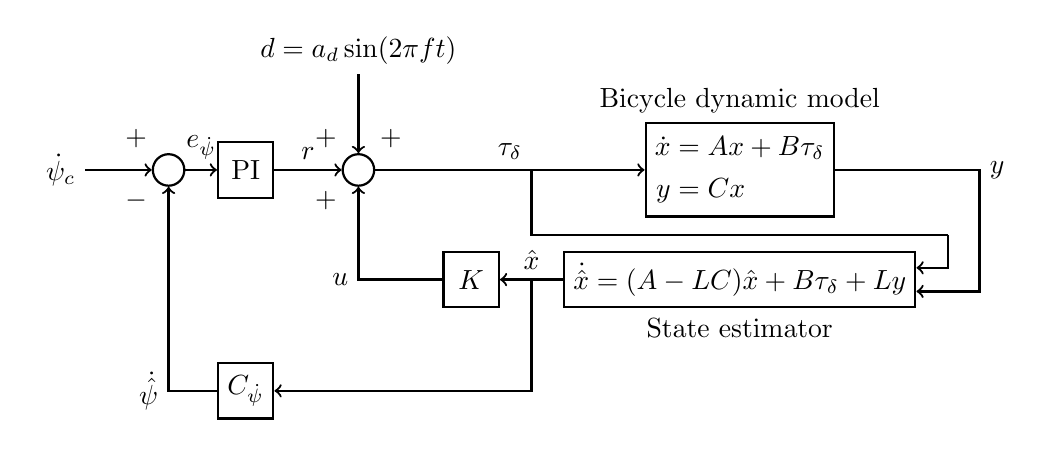
\begin{tikzpicture}[
    block/.style={rectangle,draw,thick,minimum height=2em,minimum width=2em},
    sum/.style={circle,draw,thick,inner sep=0pt,minimum size=4mm},
    connector/.style={->,thick},
    guide/.style={},
    line/.style={thick}]
    % We start by placing nodes in a 5x10 matrix
    \matrix[ampersand replacement=\&, row sep=0.2cm, column sep=0.4cm] {
    %\node (disturbance_input) [coordinate, above=of inner_sum] {};
    % First row
    \node (input) [] {$\dot{\psi}_c$}; \&
    \node (outer_sum) [sum,label=135:$+$,label=225:$-$] {}; \&
    \node (pi_block) [block] {PI}; \&
    \node (inner_sum) [sum,label=45:$+$,label=135:$+$,label=225:$+$] {}; \&
    \&
    \node (branch_1) [coordinate] {}; \&
    \node (bicycle_block) [block,label=above:Bicycle dynamic model] {
    $\begin{aligned}\dot{x} &= Ax + B\tau_\delta\\
                          y &= C x
                        \end{aligned}$}; \& \& \& \\
    % Second row
    \& \& \& \& \& \node (u_route1) [coordinate] {}; \& \& \node (u_route2)
    [coordinate] {}; \& \node(y_route) [coordinate] {}; \& \\
    % Third row
    \& \& \& \& \node (gain_block) [block] {$K$}; \& \node(branch_2)
    [coordinate] {}; \&
    \node (estimator_block) [block,label=below:State estimator] {%
      $\dot{\hat{x}} = (A - LC)\hat{x} + B\tau_\delta + Ly$}; \& \& \& \\
    % Fourth row
      \& \& \node(C_yr) [block] {$C_{\dot{\psi}}$}; \& \& \& \& \& \& \& \\
    };
    % Place disturbance node above inner_sum, not using the matrix layout
    \node (disturbance) [above=of inner_sum] {$d = a_d\sin(2\pi f t)$};

    \draw[connector] (input.east) to (outer_sum.west);
    \draw[connector] (outer_sum.east) to node[auto] {$e_{\dot{\psi}}$} (pi_block.west);
    \draw[connector] (pi_block.east) to node[auto] {$r$} (inner_sum.west);
    \draw[connector] (disturbance.south) to (inner_sum.north);
    \draw[connector] (inner_sum.east) to node[auto] {$\tau_\delta$} (bicycle_block.west);
    \draw[connector] (estimator_block.west) to node[auto,swap] {$\hat{x}$} (gain_block.east);
    \draw[connector] (gain_block.west) -| node[auto] {$u$} (inner_sum.south);
    \draw[line] (branch_1) to (u_route1) to (u_route2);
    \draw[connector] (u_route2) |- ($(estimator_block.east) + (0mm, 1.5mm)$);

    \draw[line] (bicycle_block.east) -| node[auto] {$y$} (y_route);
    \draw[connector] (y_route) |- ($(estimator_block.east) - (0mm, 1.5mm)$);

    \draw[connector] (branch_2) |- (C_yr.east);
    \draw[connector] (C_yr.west) -| node[auto] {$\dot{\hat{\psi}}$} (outer_sum.south);

  \end{tikzpicture}
  \caption{Yaw rate control block diagram. The bicycle state is $x=[\phi,
  \delta, \dot{\phi}, \dot{\delta}]$, $\hat{x}$ is the state estimate, input to
  the bicycle is steer torque $\tau_\delta$, the measurements are $y =
  [\delta, \dot{\phi}]$.}
  \label{rb:fig:yr_block_diagram}
\end{figure}
The state feedback gain $K$ was computed by discretizing the plant model and
solving the discrete algebraic Riccati equation associated with the cost
function
\begin{align}
  J &= \sum_{i=1}^{\infty} (x_i^T Q x_i + u_i^T R u_i)
\end{align}
where $Q$ and $R$ were selected to be
\begin{align}
  Q &= \text{diag}(\frac{1}{(\frac{2\pi}{180})^{2}},
                   \frac{1}{(\frac{5\pi}{180})^{2}},
                   \frac{1}{(\frac{2\pi^2}{180})^{2}},
                   \frac{1}{(\frac{100\pi^2}{180})^{2}}) \\
  R &= \frac{1}{0.5^2}
\end{align}
This choice was selected following Bryson's rule~\cite{Bryson1975}; the terms
inside the $(\cdot)^2$'s in the denominator can be viewed as the ``maximum
allowable'' value for the corresponding state or control variable (e.g., the
``maximum allowable'' value for lean $\phi$ was $\frac{2\pi}{180}=2^{\circ}$).

Once the state feedback gain was computed, the closed loop eigenvalues of the
stabilized plant dynamics $A+BK$ were computed, and the estimator gain was
selected using pole placement. The poles of the estimator were all placed on
the negative real axis, equally spaced by 0.2 rad/s, and with the slowest estimator
pole being $3\min(\text{real}(\sigma(A+BK)))$. This ensured the convergence of
the estimator was substantially faster than the controller dynamics.

With the bicycle dynamics stabilized by the inner loop, an outer loop was added
to track yaw rate. Yaw rate was chosen as the variable to track because it is a
natural way to describe both straight line motion ($\dot{\psi}=0$) as well as
steady turning motion ($\dot{\psi}=c\ne0$). The Matlab function
\verb|pidtune()| was used to compute the PI gains.

Since the dynamics of the bicycle vary with speed, this control system design
was performed at 101 speeds, logarithmically spaced between 0.5m/s and 10m/s.
All matrices in \autoref{rb:fig:yr_block_diagram} were output to a C++ file as
an array of matrices parameterized by speed. This file was then compiled into
the firmware and gain scheduling was used to compute the actual control law
based on the measured speed. A linear interpolation of the state update and
control law were performed using the nearest two speeds to the measured speed.
An implication of this is that estimation and control was not possible below
0.5m/s. This turned out not to be a problem as long as the bicycle was started
from a standstill near the upright reference configuration.

\subsection{User interface} \label{rb:subsec:ui}
The following list details the available commands and gives a brief description
of each.

\begin{description}
  \item[\Q{collect [filename]}] Begin main data collection and control loop and store
    data in optional argument \verb|filename| (if not supplied, data is stored in
    \verb|samples.dat|).
  \item[\Q{disable}] Immediately disable the motors and end data collection.
  \item[\Q{reset}] Perform a software reset of the microcontroller.
  \item[\Q{threads}] Show the memory address, stack address, priority, number
    of references to this thread, thread state, thread time in ticks, and the
    name of all currently running threads.
  \item[\Q{calibrate}] Begin the steer angle calibration routine (see
    \autoref{rb:subsec:sensors})
  \item[\Q{homefork}] Wait for the steer encoder index signal to set the steer calibration offset.
  \item[\Q{e_thresh v_e}] Set state estimation threshold speed to \verb|v_e| m/s.
    \verb|v_e| must be greater than or equal to 0.5m/s (the lowest speed
    for which linearized bicycle dynamics state space matrices were generated).
  \item[\Q{c_thresh v_c}] Set the threshold speed to \verb|v_c| m/s. Once the
    bicycle speed \verb|v| exceeds \verb|v_c| yaw rate control is enabled. Must
    be larger than estimation threshold speed.
  \item[\Q{thresh v_e v_c}] Simultaneously set state estimation and control threshold speeds.
  \item[\Q{disturb a_d f}] Set disturbance amplitude to \verb|a_d|\num{1e-2}Nm
    and disturbance frequency to \verb|f| Hz (see
    \autoref{rb:fig:yr_block_diagram}).
  \item[\Q{speed v}] Set commanded speed in m/s. The control system will
    immediately attempt to track this speed until a fault occurs or the
    reference is changed by the user. On reset, the reference speed is set 0
    m/s.
  \item[\Q{speed_limit v d}] Set commanded speed to \verb|v| m/s and distance
    limit to \verb|d| meters. This works the same as \verb|speed| except that
    once the bicycle has travelled \verb|d| meters, the commanded speed is
    changed to 1.0 m/s, a speed which was easy to walk next to and catch the
    bicycle.
  \item[\Q{l_thresh t}] Set the lateral acceleration threshold to \verb|t|. At
    the beginning of each run, a green LED is illuminated when the bicycle
    lateral acceleration is below \verb|t| (with a default of \verb|t|=0.01
    m/s$^2$). This enables the bicycle to be initialized with as close to zero
    lean angle as possible. The sensed lateral acceleration is non-zero in
    static conditions because the accelerometer senses the gravitational field.
  \item[\Q{yaw_rate yr}] Set the commanded yaw rate in rad/s. On
    reset, reference yaw rate is 0 rad/s (straight line motion).

\end{description}

\section{Results} \label{rb:sec:experiments}

\subsection{Experiments conducted} \label{rb:subsec:experiments}
On July 13, 2013, twenty eight experimental runs were performed on the Dairy
Road basketball courts of the UC Davis campus (38.53794$^{\circ}$ North,
121.759475$^{\circ}$ West). Oliver Lee and Dr. Mont Hubbard were stationed at the
northeast corner of the east court, while I travelled east and west with the
robot bicycle each run. To begin each run, Oliver Lee operated the laptop and
issued commands to configure the filename (following a naming convention $<$run
number$>$.dat), speed set point, distance to travel before reducing the speed
set point to 1.0 m/s, and optionally, an additive sinusoidal disturbance steer
torque of magnitude $a_d$ cNm and frequency $f_d$ Hz. Dr. Hubbard took notes
about each run and coordinated with Oliver Lee to ensure commands issued to robot
were consistent with his notes. Prior to issuing a non-zero speed set point
command, I held the bicycle near the reference configuration (as indicated by
two LED's which turned on when IMU lateral acceleration and steer angle were
less than 0.01 m/s$^2$ and 1.0 deg, respectively), then ran along side the
bicycle as it travelled east to west or west to East. At the end of each run, I
would turn of the main power switches to each motor and catch the bicycle to
prevent it from falling on its casters.  The speed command issued by Oliver
took two arguments: speed set point and distance to travel before changing the
set point to 1.0 m/s. At 1.0 m/s, it was easy to manually switch off the motors
and catch the bicycle.
\begin{center}
  \begin{longtable}{| l | l | l | l | l | l | l |}
  \hline
  Run & Time (PST) & Speed (m/s) & $A_d$ (cNm) & $f_d$ (Hz) & $x$ (m) &
  Direction \endhead
  \hline
  \multicolumn{7}{|p{\textwidth}|}{Yaw rate PI controller is designed such that
  first 0dB cross-over frequency is 0.1 Hz. Additive disturbance torque is
  $\sin\left(2\pi t \right)$.} \\
  \hline
  000 & 0641 & 2.0 & -- & -- & 30.0 & West \\
  \hline
  001 & 0643 & 2.0 & -- & -- & 30.0 & West \\
  \hline
  002 & 0644 & 3.0 & -- & -- & 30.0 & East \\
  \hline
  003 & 0646 & 3.0 & -- & -- & 30.0 & West \\
  \hline
  004 & 0647 & 4.0 & -- & -- & 30.0 & East \\
  \hline
  005 & 0649 & 4.0 & -- & -- & 30.0 & West \\
  \hline
  006 & 0650 & 4.0 & -- & -- & 60.0 & East \\
  \hline
  007 & 0652 & 4.0 & -- & -- & 60.0 & East \\
  \hline
  008 & 0656 & 2.0 & 0.5 & 1.0 & 30.0 & West \\
  \hline
  009 & 0659 & 2.0 & 1.0 & 1.0 & 30.0 & East \\
  \hline
  010 & 0701 & 2.0 & 1.0 & 1.0 & 30.0 & East \\
  \hline
  \multicolumn{7}{|p{\textwidth}|}{Changed additive disturbance torque to be
  $A_d \sin\left(2\pi f_d \left(t - t_i\right)\right)$, where $t_i$ is the time at which
  the disturbance is initially applied.} \\
  \hline
  011 & 0714 & 2.0 & 1.0 & 1.0 & 30.0 & West \\
  \hline
  012 & 0718 & 2.0 & 5.0 & 1.0 & 30.0 & East \\
  \hline
  013 & 0721 & 2.0 & 5.0 & 1.0 & 30.0 & West \\
  \hline
  014 & 0725 & 2.0 & -5.0 & 1.0 & 30.0 & East \\
  \hline
  \multicolumn{7}{|p{\textwidth}|}{Changed yaw rate PI controller design such that
  first 0dB cross-over frequency is selected by Matlab's
  pidtune() instead of specified to be 0.1 Hz} \\
  \hline
  015 & 0754 & 2.0 & -- & -- & 30.0 & West \\
  \hline
  016 & 0756 & 2.0 & -- & -- & 30.0 & East \\
  \hline
  017 & 0757 & 4.0 & -- & -- & 30.0 & West \\
  \hline
  018 & 0800 & 2.0 & 5.0 & 1.0 & 30.0 & East \\
  \hline
  019 & 0808 & 2.0 & 5.0 & 5.0 & 30.0 & West \\
  \hline
  020 & 0813 & 2.0 & 10.0 & 1.0 & 30.0 & West \\
  \hline
  021 & 0815 & 2.0 & -- & -- & 30.0 & West \\
  \hline
  022 & 0816 & 1.0 & -- & -- & 30.0 & East \\
  \hline
  023 & 0818 & 1.0 & -- & -- & 30.0 & East \\
  \hline
  024 & 0821 & 2.0 & -- & -- & 5.0 & East \\
  \hline
  025 & 0824 & 2.0 & -- & -- & 60.0 & West \\
  \hline
  026 & 0825 & 3.0 & -- & -- & 50.0 & East \\
  \hline
  027 & 0827 & 3.0 & -- & -- & 50.0 & East \\
  \hline
  028 & 0829 & 3.0 & -- & -- & 50.0 & East \\
  \hline
  \end{longtable}

\end{center}


\subsection{Results} \label{rb:subsec:results}

\subsection{Discussion} \label{rb:subsec:discuss}




%
%\section{Yaw rate controller}
%The objective of the yaw rate controller is twofold: 1) stabilize the roll and
%steer dynamics, and 2) track a reference yaw rate $\dot{\psi}_r$.  Because the
%lateral dynamics are dependent on $\dot{\theta}_R$, yaw rate controller gains
%were computed at 101 values of $\dot{\theta}_R$, logarithmically spaced between
%$10^{-0.5}$ and $10^1$ m / s. Using logarithmic spacing instead of linear
%spacing has the effect of providing relatively higher controller gain density
%at lower speeds than at higher speeds. This is important because the bicycle is
%relatively more unstable at lower speeds than at higher speeds and the unstable
%dynamics change with speed more quickly below the weave critical speed than
%they do above the capsize speed.  Put simply, a bicycle is more difficult to
%balance at low speeds and careful gain selection is more important at low
%speeds than at high speeds.
%
%The yaw rate controller has four measurements which are used to compute the
%applied steer torque: 1) rear wheel rate, 2) steer angle, 3) roll rate, and 4)
%yaw rate. First, the rear wheel rate measurement is used to look up the
%controller gains which were designed for the bicycle in forward steady cruise
%with rear wheel rates above and below the measurement.  The remaining three
%measurements are used as inputs to the state equations (at each speed).  The
%two state updates are linearly interpolated at the current speed measurement to
%obtain the actual state update.  This interpolated state update is then used to
%compute the output steer torque.
%
%The design of the controller (at each speed) involves two independent steps: 1)
%solve the discrete algebraic Riccati equation (DARE) associated with a LQR
%optimal control problem to compute the optimal state feedback gain, and 2)
%solve the DARE associated with an optimal estimation problem to compute the
%optimal filter gain which is used to compute the state estimate. The state
%estimate is then used in place of the true state in the LQR controller. The
%design of the controller and estimator are described below.
%
%\subsection{LQR yaw rate controller with integral action}
%The four states of the bicycle model are roll $\phi$, steer $\delta$, roll rate
%$\dot{\phi}$, and, steer rate $\dot{\delta}$.  These four states are augmented
%with a fifth state, the time integral of yaw rate error
%$\int\dot{\psi}-\dot{\psi}_r dt$.  This five dimensional state is denoted by
%$x_k$. A block diagram of the state feedback control topology is shown below.
%
%\begin{tikzpicture}[auto, node distance=2cm,>=latex']
%  % We start by placing the blocks
%  \node [input, name=input] {};
%  \node [sum, right of=input] (sum) {};
%  \node [block, right of=sum] (integrator) {$\frac{T_s}{z-1}$};
%  \node [block, right of=integrator] (gain) {$K_c$};
%  \node [block, right of=gain] (bicycle) {Bicycle};
%  % We draw an edge between the controller and system block to 
%  % calculate the coordinate u. We need it to place the measurement block. 
%  \draw [->] (sum) -- node[name=e] {$e$} (integrator);
%  \draw [->] (integrator) -- node[name=xi] {} (gain);
%  \draw [->] (gain) -- node[name=u] {$\tau_{\delta}$} (bicycle);
%  \node [output, right of=bicycle] (output) {};
%  \coordinate [above of=u] (tmp1);  % 
%  \coordinate [below of=xi] (tmp2);  % 
%
%  % Once the nodes are placed, connecting them is easy. 
%  \draw [draw,->] (input) -- node {$\dot{\psi}_r$} (sum);
%  %\draw [->] (sum) -- node {$e$} (controller);
%  \draw [->] (bicycle) -- node [name=y] {$\dot{\psi}$} (output);
%  %\draw [->] (y) -- (tmp1) -- (gain);
%  \draw [->] (y) |- (tmp2) -| node[pos=0.99] {$-$} (sum);
%\end{tikzpicture}
%
%TODO: Finish block diagram
%
%\begin{align}
%\label{eq:augmented_plant}
%    x_{k+1} & =
%  \begin{bmatrix}
%    A & 0 \\
%    -C_{\dot{\psi}} T_s & 1
%  \end{bmatrix}
%    x_{k} +
%  \begin{bmatrix}
%    B_{\delta} \\ 0
%  \end{bmatrix}
%    u_k \\
%\label{eq:augmented_plant_simple}
%  & = A_{cp} x_{k} + B_{cp} u_k
%\end{align}
%The $A$ matrix is the bicycle system dynamics matrix, $B_{\delta}$ is the
%bicycle input matrix associated with steer torque inputs, and, $C_{\dot{\psi}}$
%is the output matrix associated with measurement of yaw rate $\dot{\psi}$, all
%converted to discrete time using sample time $T_s$.  Subscript ``cp'' denotes
%``controlled plant''.
%
%The controller seeks the sequence of control inputs $u^*_k$, $k \geq 0$, which
%minimizes the quadratic cost function
%\begin{align}
%  J(u) = \sum_{k=0}^{\infty} x_k^T Q x_k + r u_k^2
%\label{eq:LQRcost}
%\end{align}
%for any initial state $x_0$. $Q \in \mathbf{R}^{5 \times 5}, Q = Q^T \geq 0$
%is the state weighting matrix, and $r$ is the positive real control control
%weighting. The solution to the optimal control problem is the linear state
%feedback
%\begin{align}
%\label{eq:linear_state_feedback}
%u^*_k & = -(r + B_{cp} P^*_c B_{cp})^{-1} B_{cp}^T P_c^* A_{cp} x_k \\
%      & = K_c x_k
%\end{align}
%where $P^*_c$ is the the unique, symmetric positive definite solution of the
%DARE
%\begin{align}
%\label{eq:DARE_controller}
%A_{cp}^T (P_c - P_c B_{cp} (r + B_{cp}^T P_c B_{cp})^{-1} B_{cp}^T
%P_c) A_{cp} + Q & = 0
%\end{align}
%The linear state feedback gain $K_c \in \mathbf{R}^{1 \times 5}$ stabilizes the
%bicycle and provides zero steady state tracking error to a reference yaw rate.
%This gain is computed at each speed with the following $Q$ and $r$ weightings
%\begin{align}
%Q &= \mathrm{diag}(1, 1, 1, 1, 1) \\
%r &= 1
%\end{align}
%TODO: plot of LQR weightings vs. rear wheel rate.
%
%\subsection{State estimator}
%The state estimator is designed to estimate the five states in
%\ref{eq:augmented_plant_simple}. The state equations must be modified to
%include the input reference yaw rate and the measurement equations. The state
%and output equations of the plant to be estimated are
%\begin{align}
%    x_{k+1} & =
%  \begin{bmatrix}
%    A & 0 \\
%    -C_{\dot{\psi}} T_s & 1
%  \end{bmatrix} x_{k} +
%  \begin{bmatrix}
%    B_{\delta} & 0 \\ 0 & T_s
%  \end{bmatrix}
%  \begin{bmatrix}
%    u_k \\ r_k
%  \end{bmatrix}
%  + w_k \\
%  & = A_{ep} x_k + B_{ep} \begin{bmatrix} u_k \\ r_k \end{bmatrix} + w_k \\
%  y_k & =
%  \begin{bmatrix}
%    0 & 1 & 0 & 0 & 0\\ % Steer angle measurement
%    0 & 0 & 1 & 0 & 0\\ % Roll rate measurement
%    0 & 0 & 0 & 0 & 1    % Integral of yaw rate error measurement
%  \end{bmatrix}
%    x_{k} + v_k \\
%  &= C_{ep} x_k + v_k
%\label{eq:estimated_plant}
%\end{align}
%where the subscript ``ep'' denotes ``estimated plant'', $C_m \in \mathbf{R}^{2\times4}$ represents the measurement output matrix
%associated with measuring steer angle and roll rate.  The third output of this
%plant is integral of yaw rate error, which we assume to have a direct
%measurement of.  Process noise $w_k$ and measurement noise $v_k$ are assumed to
%have zero mean and covariance $W$ and $V$ respectively.
%
%The state estimate is computed in two steps: a prediction step that
%extrapolates the state estimate based on assumed dynamics, and a correction
%step which uses the most recent measurements.  The two steps are
%\begin{align}
%  \hat{x}_{k+1} & = A_{ep} \bar{x}_k + B_{ep} \begin{bmatrix} u_k \\ r_k \end{bmatrix} \\
%  \bar{x}_{k+1} & = \hat{x}_{k+1} + K_e (y_{k+1} - C_{ep} \hat{x}_{k+1})
%\end{align}
%These can be combined into a single state space equation
%\begin{align}
%\bar{x}_{k+1} & = (I - K_e C_{ep}) A_{ep} \bar{x}_k
%            + \begin{bmatrix}(I - K_e C_{ep}) B_{ep} & K_e \end{bmatrix}
%              \begin{bmatrix} u_k \\ r_k \\ y_{k+1} \end{bmatrix}
%\end{align}
%Where $K_e$ is the estimator gain. In order for the estimator states to
%converge to the true state, the error dynamics must be stable.  The error
%dynamics are
%\begin{align}
%  \bar{e}_{k+1} & \triangleq x_{k+1} - \bar{x}_{k+1} \\
%  & = A_{ep} x_k + B_{ep} \begin{bmatrix} u_k \\ r_k \end{bmatrix} - (I - K_e C_{ep}) A_{ep} \bar{x}_k
%    - \begin{bmatrix}(I - K_e C_{ep}) B_{ep} & K_e \end{bmatrix}
%              \begin{bmatrix} \tilde{u}_k \\ \tilde{y}_{k+1} \end{bmatrix} \\
%              & = (I - K_e C_{ep}) A_{ep} (x_k - \bar{x}_k) \\
%              & = (I - K_e C_{ep}) A_{ep} \bar{e}_k
%\label{eq:estimator_error}
%\end{align}
%The error dynamics are stable if and only if $(I - K_e C_{ep}) A_{ep}$ has all
%eigenvalues inside the closed unit circle.  The pair $(A_{ep}, C_{ep} A_{ep})$
%must be observable for arbitrary eigenvalue assignment.
%
%The estimator gain $K_e$ is chosen to be
%\begin{align}
%K_e & = P_e^* C_{ep}^T (C_{ep} P_e^* C_{ep}^T + V)^{-1}
%\end{align}
%where $P_e^*$ is the unique, symmetric, positive definite solution of the
%DARE
%\begin{align}
%\label{eq:DARE_observer}
%A_{ep}(P_e - P_e C_{ep}^T(C_{ep} P_e C_{ep}^T + V)^{-1} C_{ep} P_e) A_{ep}^T -
%P_e + W &= 0
%\end{align}
%The solution to the DARE was found using the Schur vector technique of Laub
%\cite{Laub1979}
%
%\subsection{Closed loop dynamics}
%The bicycle state equations along with the estimator state equations are
%\begin{align}
%x_{k+1} & = A_{ep} x_k + B_{ep} \begin{bmatrix} u_k \\ r_k \end{bmatrix} \\
%\bar{x}_{k+1} & = (I - K_e C_{ep}) A_{ep} \bar{x}_k +
%  \begin{bmatrix} (I - K_e C_{ep}) B_{ep} & K_e \end{bmatrix}
%  \begin{bmatrix} u_k \\ r_k \\ y_{k+1} \end{bmatrix}
%\end{align}
%Using the feedback law $u_k = K_c \bar{x}_k$ and the measurement equations
%$y_{k+1} = C_{ep} x_{k+1}$, the closed loop dynamics of the combined system
%becomes
%\begin{align}
%  x_{k+1} & = A_{ep} x_k + \begin{bmatrix} B_{\delta} \\ 0 \end{bmatrix} K_c
%  \bar{x}_k + \begin{bmatrix} 0 \\ T_s \end{bmatrix} r_k \\
%  \bar{x}_{k+1} & = K_e C_{ep} A_{ep} x_k + \begin{bmatrix} (I - K_e C_{ep})
%  A_{ep} + \begin{bmatrix} B_{\delta} \\ 0 \end{bmatrix} K_c \end{bmatrix}
%  \bar{x}_k + \begin{bmatrix} 0 \\ T_s \end{bmatrix} r_k
%\end{align}
%
%\subsection{Implementation}
%Since the controller design has an augmented state that is not part of the
%bicycle, and this state is not measured from a physical sensor, both this
%``measurement'' loop, and the control loop, can be closed in the implementation
%of the controller.  The resulting state space equations have five states (four
%bicycle state estimates and the integral of yaw rate error), three inputs (yaw
%rate reference, steer angle measurement, and roll rate measurement), and, one
%output (steer torque).
%
%
%
%\section{Introduction}
%
%\section{System identification experiments}

\printbibliography[section=4,heading=subbibliography]
\chapter{Conclusions and suggestions for future work}
The nonlinear equations of motion for the bicycle model described in
\hyperref[chapter2]{Chapter 2} were formulated using bicycle gyrostat
parameters and subsequently linearized using the linearization procedure
described in \hyperref[chapter3]{Chapter 3}. These linearized equations were
found to match previously published eigenvalues for a set of benchmark
parameters, thereby establishing that no mistakes were made in the derivation.
However, this does not establish the soundness of the modelling assumptions.
The use of the linearized dynamic equations to design a control system that
balances the bicycle both in simulation and in practice does however, to some
degree, establish that the Whipple bicycle model is at least descriptive for a
control system based upon its assumptions to keep an unmanned bicycle from
falling over. To what degree the Whipple model is accurate and how exactly to
quantify the degree to which it is accurate was not concretely established by
this work.

There are several areas where this issue can be addressed. A more careful
measurement of all of the physical parameters of the bicycle would be an
inexpensive way to improve the knowledge of the assumed plant. At the some
time, issues such as inertial asymmetries of the four rigid bodies in the real
bicycle should be either eliminated or, if it is not possible to eliminate
entirely, quantified. This may necessitate the need to reformulate the model of
\hyperref[chapter2]{Chapter 2} to include inertial asymmetries. A change to
the model such as allowing for the mass center of the frame and fork to lie
outside the plane of the wheel, would be a simple addition, and similar such
modifications could be added if necessary. Other improvements in the design of the
state estimator (i.e., a reduced order observer) would also be worth testing to
see if they improve the performance characteristics of the controller. A final
high value, low cost, would be to use a higher resolution optical encoder (a
drop in replacement encoder exists that would yield 20000 quadrature counts per
wheel revolution). This improvement would to reduce discretization jitter in
the speed measurement which in turn would reduce jitter in the gain scheduling
lookup. It is unclear whether this concern is actually justified, but
nevertheless, it is a simple and cheap fix.

The goal of applying additive sinusoidal disturbance steer torques as a means
to excite specific frequencies did not work as well as planned. One problem was
that a zero mean disturbance steer torque caused a non-zero mean yaw rate,
despite the yaw rate command of zero. This may be addressable by refinement of
the control system and how the disturbance signal is applied.

Commanding circular motions (i.e., $\dot{\psi}_c \ne 0$) of the robotic bicycle
was not attempted due to lack of space and time. The theory of steady turning
bicycles is less developed than that of bicycles travelling in a straight line,
so there is substantial room for investigations of steady turns, both in terms
of numerical studies of the model, as well as experimental validations of the
model in operating conditions other than upright steady forward cruise.

With the improvements mentioned, more rigorous system identification
experiments would be possible and the validity of the inadequacies of the
Whipple model could be more precisely quantified. It is my suspicion that the
lack of a tire model is likely the first place to look when making improvements
to the model, though there may be other simple additions to the model, such as
using the torus model of the wheel instead of the knife edged model that could
potentially improve model fidelity. Simple models of tires do exist and can be
be added to the bicycle model easily to determine how far a simple tire model
can be taken. If more sophisticated tire models prove necessary, measurement of
tire viscoelastic properties would required.

This dissertation, as with any work, is never fully ``finished''. The \LaTeX{}
source code, scripts, images, and data used for generating figures is available
online~\cite{Peterson2013}.


\printbibliography[section=5,heading=subbibliography]

\UMIabstract[This dissertation explores bicycle dynamics through an extension of the Whipple
bicycle model and validation of the model equations equations of motion through
the implementation of a robotic bicycle. An extended Whipple bicycle model is
presented which makes uses of a unique set of physical parameters based on
cylindrical gyrostats. The nonlinear equations of motion for this model are
derived, linearized, and validated against a set of benchmark model parameters.
A general formulation for the linearization of a system with configuration and
velocity constraints is presented, and is demonstrated on an idealized rolling
disk. The method of linearization is directly applicable to the equations of
motion which result from the application of Kane's method. The linearization
procedure is used to formulate the linear state space equations of motion for
the bicycle model, which are then used as the plant model to design the robotic
bicycle control system. The mechanical, electrical, and software aspects of the
robotic bicycle are presented, along with representative results from a set of
experiments.

]

\end{document}

